%%%%%%%%%%%%%%%%%%%%%%%%%%%%%%%%%%%%%%%%%%  不使用 authblk 包制作标题  %%%%%%%%%%%%%%%%%%%%%%%%%%%%%%%%%%%%%%%%%%%%%%
%-------------------------------PPT Title-------------------------------------
\title{分子动力学方法与应用简介}
%-----------------------------------------------------------------------------

%----------------------------Author & Date------------------------------------
%\author[\textrm{Jun\_Jiang}]{姜\;\;骏\inst{}} %[]{} (optional, use only with lots of authors)
%% - Give the names in the same order as the appear in the paper.
%% - Use the \inst{?} command only if the authors have different
%%   affiliation.
\institute[BCC]{\inst{}%
%\institute[Gain~Strong]{\inst{}%
\vskip -20pt 北京市计算中心~云平台事业部~姜骏}
%\vskip -20pt {\large 格致斯创~科技}}
\date[\today] % (optional, should be abbreviation of conference name)
{	{\fontsize{6.2pt}{4.2pt}\selectfont{\textcolor{blue}{E-mail:~}\url{jiangjun@bcc.ac.cn}}}
\vskip 45 pt {\fontsize{8.2pt}{6.2pt}\selectfont{北京科技大学~~理化楼-\textrm{308}% 报告地点
	\vskip 5 pt \textrm{2024.07.12}}}
}

%% - Either use conference name or its abbreviation
%% - Not really information to the audience, more for people (including
%%   yourself) who are reading the slides onlin%%   yourself) who are reading the slides onlin%%   yourself) who are reading the slides onlineee
%%%%%%%%%%%%%%%%%%%%%%%%%%%%%%%%%%%%%%%%%%%%%%%%%%%%%%%%%%%%%%%%%%%%%%%%%%%%%%%%%%%%%%%%%%%%%%%%%%%%%%%%%%%%%%%%%%%%%

\subject{}
% This is only inserted into the PDF information catalog. Can be left
% out.
%\maketitle
\frame
{
%	\frametitle{\fontsize{9.5pt}{5.2pt}\selectfont{\textcolor{orange}{“高通量并发式材料计算算法与软件”年度检查}}}
\titlepage
}
%-----------------------------------------------------------------------------

%------------------------------------------------------------------------------列出全文 outline ---------------------------------------------------------------------------------
\section*{}
\frame[allowframebreaks]
{
  \frametitle{Outline}
%  \frametitle{\textcolor{mycolor}{\secname}}
  \tableofcontents%[current,currentsection,currentsubsection]
}
%%在每个section之前列出全部Outline
%%类似的在每个subsection之前列出全部Outline是\AtBeginSubsection[]
%\AtBeginSection[]
%{
%  \frame<handout:0>%[allowframebreaks]
%  {
%    \frametitle{Outline}
%%全部Outline中,本部分加亮
%    \tableofcontents[current,currentsection]
%  }
%}

%-----------------------------------------------PPT main Body------------------------------------------------------------------------------------
\small
\section{分子动力学基础}
\frame
{
	\frametitle{分子模拟}
	分子模拟:~\textcolor{blue}{研究原子分子层次的物性}
	\begin{itemize}
		\item 分子模拟方法分为~\textrm{Monte~Carlo~(MC)}和\textrm{Molecular~Dynamics~(MD)}两大类
		\item \textcolor{blue}{统计物理}是理论基础:~\textrm{Boltzmann}分布的重要性采样
	\end{itemize}
	\begin{itemize}
		\item 量子效应只有在粒子波长$\lambda$与原子间距离\textrm{(1-3~\AA)}相当时才变得重要:~\textcolor{blue}{一般原子/分子的运动,用经典力学足以精确描述}
			\vskip 2pt
			尽管第一性原理方法在功能材料,特别是光电磁相关研究领域中独树一帜,但是大多数与原子/分子运动相关的材料——\textcolor{blue}{典型的如结构材料}——研究,主要应用经典力学预测%特别是对于结构材料,如何利用分子动力学方法来描述材料中的原子运动是该领域的重要主题。
		\item 自\textrm{1950}年代,\textrm{Alder}和\textrm{Wainwright}通过密堆积球出发,成功模拟液-固相变%\upcite{JCP27-1208_1957}
			开始,标志着分子动力学方法成功应用到材料学模拟中
			%自此以后,大量的高效算法和代码以及不断升级的计算能力使得分子动力学在材料领域发挥的作用日益凸显,进入21世纪,\textrm{Kadau}等实现了对3200亿个原子的分子动力学模拟\cite{IJMPC17-1755_2006},显示出该方法的巨大能力。
	\end{itemize}
	分子模拟:~\textcolor{red}{计算材料研究领域最重要的理论工具之一}
}

\frame
{
	\frametitle{\textrm{Monte~Carlo}模拟}
\begin{minipage}{0.33\textwidth}
%\begin{figure}[h!]
%\centering
%\vspace{-8.0pt}
%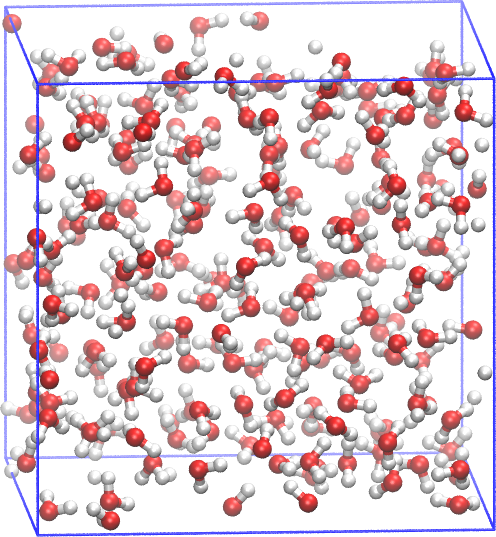
\includegraphics[height=1.45in,width=1.50in,viewport=0 0 140 138,clip]{Figures/Unit_Cell_of_Liquid_Water.png}
%\caption{\textrm{\tiny Schematic representation of water can be simulated using Periodic Boundary Conditions.}}
%\label{Water-PBC}
%\end{figure}
\begin{itemize}
\vspace{-8.0pt}
{\fontsize{9.5pt}{6.2pt}\selectfont{
	\item 基于\textrm{Boltzmann}分布,只能模拟平衡态体系
	\item 只计算势能(状态函数),不用计算力(瞬时作用)
\item 模拟步长可以比较大}}
\end{itemize}
\end{minipage}
\begin{minipage}{0.65\textwidth}
\begin{figure}[h!]
\centering
\vspace{-5.0pt}
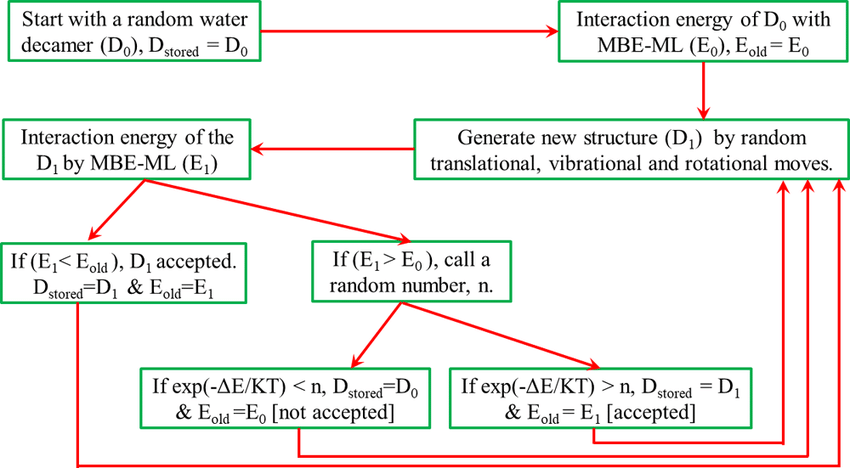
\includegraphics[height=1.55in,width=3.00in,viewport=0 0 930 475,clip]{Figures/Schematic-representation-of-the-Metropolis-Monte-Carlo-simulation.png}
%\caption{\textrm{Schematic representation of the Metropolis−Monte Carlo simulation.}}
\label{MC-Algorithm-Workflow}
\end{figure}
\end{minipage}
\begin{figure}[h!]
\centering
\vspace{-10.0pt}
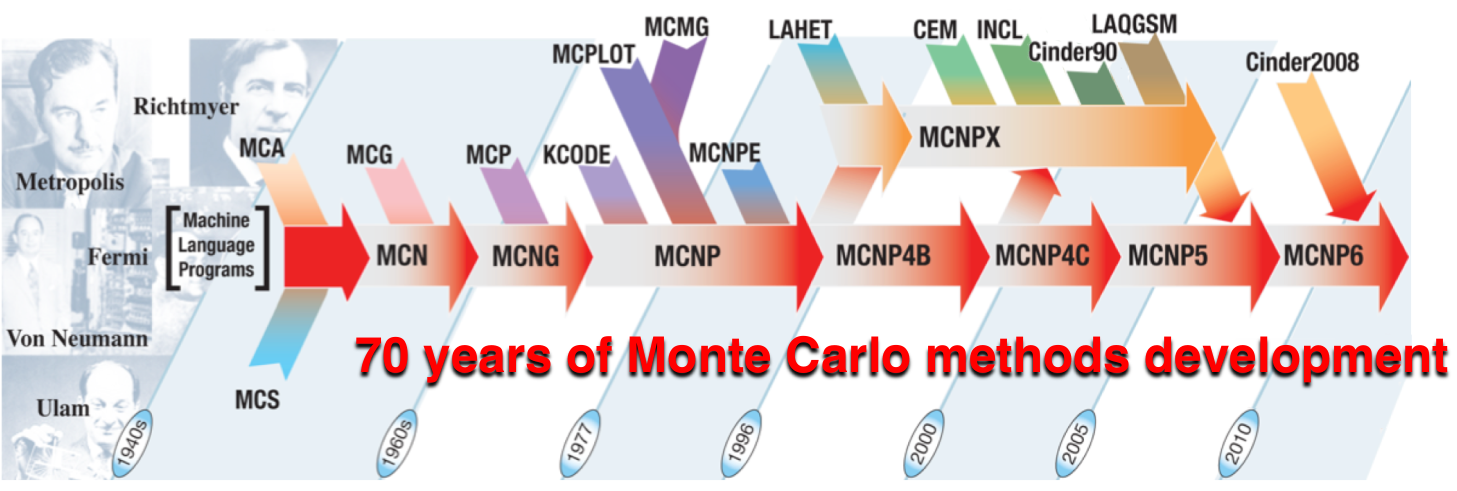
\includegraphics[height=1.25in,width=4.15in,viewport=0 0 1470 480,clip]{Figures/Monte-Carlo-development.png}
%\caption{\textrm{Schematic representation of the Metropolis−Monte Carlo simulation.}}
\label{Monte-Carlo-development}
\end{figure}
}

%\subsection{经典分子动力学提要}
\frame
{
	\frametitle{}
\begin{figure}[h!]
\centering
\vspace{-7.0pt}
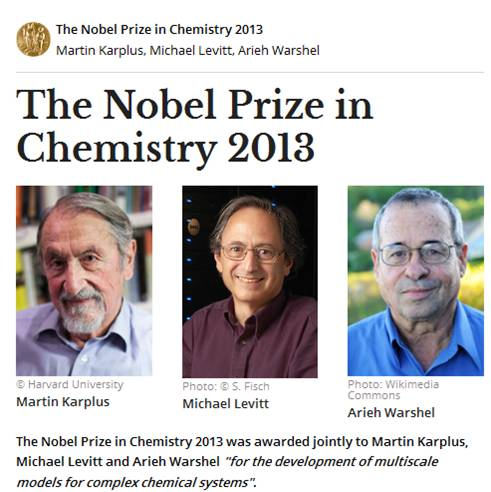
\includegraphics[height=2.85in,width=3.80in,viewport=0 0 410 300,clip]{Figures/Nobel_Prize_Chemistry-2013.jpg}
%\caption{\textrm{Schematic representation of the Metropolis−Monte Carlo simulation.}}
\label{Nobel-Prize-Chemistry_2013}
\end{figure}
}

\frame
{
	\frametitle{经典分子动力学}
\begin{minipage}{0.45\textwidth}
\begin{figure}[h!]
\centering
\vspace{-3.0pt}
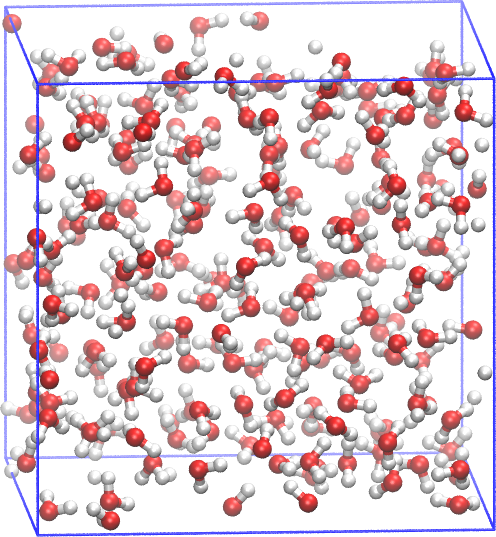
\includegraphics[height=2.00in,width=2.00in,viewport=0 0 135 135,clip]{Figures/Unit_Cell_of_Liquid_Water.png}
%\caption{\textrm{Schematic representation of the Metropolis−Monte Carlo simulation.}}
\label{Unit_Cell_of_Liquid_Water}
\end{figure}
\end{minipage}
\begin{minipage}{0.53\textwidth}
	\begin{itemize}
		\item 应用数值方法解析多粒子体系(原子、离子、$\cdots$)运动
		\item 粒子间相互作用可用简洁的解析函数或数值描述
		\item 广泛应用于材料科学、物理化学和生物科学的相关研究
		\item 模拟体系的粒子数规模:~\\$100\sim10^6$
		\item 模拟体系的时间范围:~\\$10~\mathrm{ps}\sim1\mu\mathrm{s}$~(一般是$\mathrm{ns}$范围)
	\end{itemize}
\end{minipage}
\begin{itemize}
	\item 分子动力学模拟可以包括温度和压力效应
	\item 分子动力学可以模拟相对大的体系和相对长的时间
	\item 分子动力学可以得到分子尺度的结构和动力学信息
\end{itemize}
}

\frame
{
	\frametitle{经典分子动力学}
	分子动力学方法的\textcolor{red}{优点}:
	\begin{itemize}
			\setlength{\itemsep}{5pt}
		\item 可以模拟大规模分子系统,原则上能计算系统的微观、宏观物理量,增补实验数据的空缺
		\item 与\textrm{Monte Carlo}方法相比,具备更高的准确度,可以提供更多微观粒子的运动细节
		\item 可以模拟非平衡态的体系以及体系在极端条件下复杂情况下的物理性质和物理状态
	\end{itemize}
	分子动力学方法的\textcolor{red}{缺点}:
	\begin{itemize}
			\setlength{\itemsep}{5pt}
		\item 只能描述原子(核)的运动,但无法反映电子的运动,难以准确模拟化学键
		\item 数值模拟依赖经验力场,化学环境复杂的体系,如化学键断裂,电子结构将由稳态电子结构过渡到过渡态,无法用简单的解析力场描述
	\end{itemize}
}

\frame
{
	\frametitle{经典力学\textrm{Classical Mechanics}}
\begin{figure}[h!]
\vspace*{-0.18in}
\centering
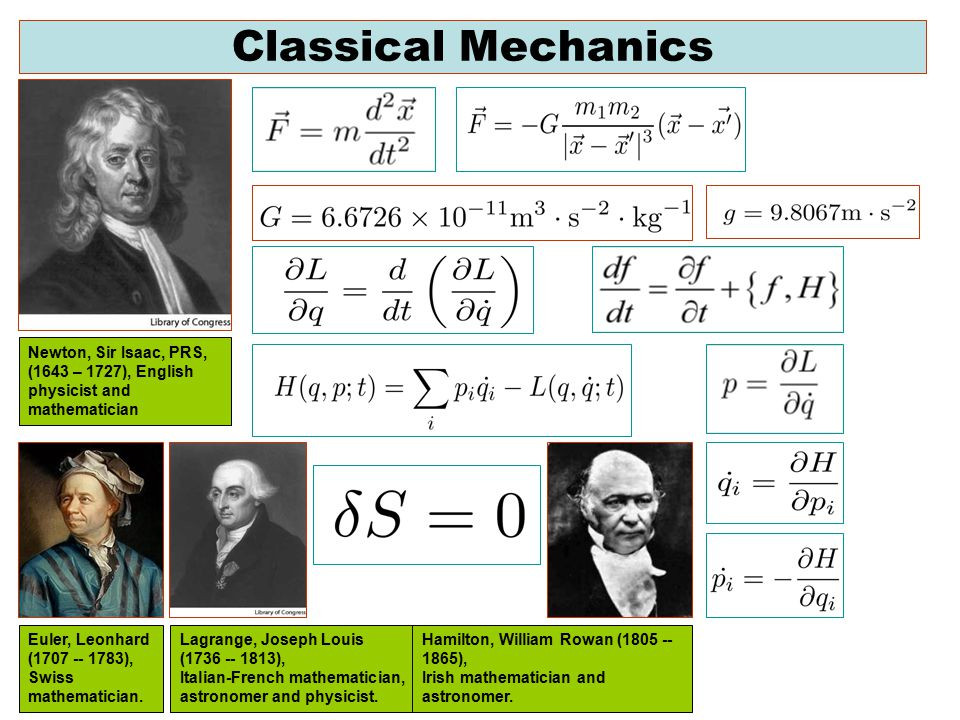
\includegraphics[height=2.65in,width=4.05in,viewport=0 0 715 495,clip]{Figures/Classical_Mechanics.jpg}
%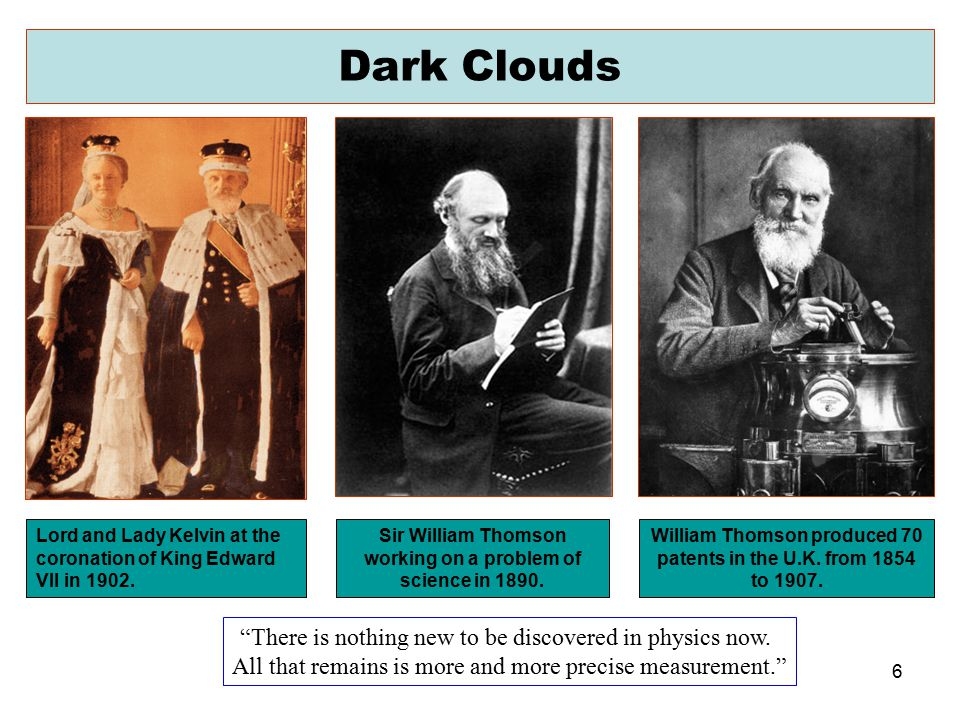
\includegraphics[height=2.50in,width=4.05in,viewport=0 20 735 470,clip]{Figures/Two-dark-cloud-in-physics-3.jpg}
%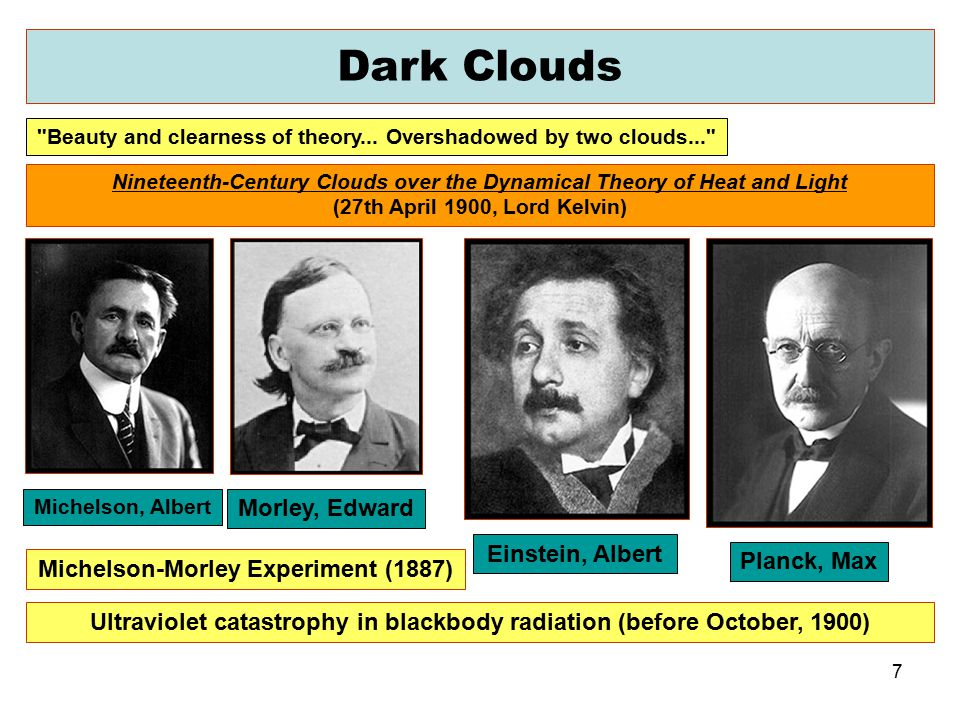
\includegraphics[height=2.40in,width=4.05in,viewport=0 50 735 470,clip]{Figures/Two-dark-cloud-in-physics-2.jpg}
%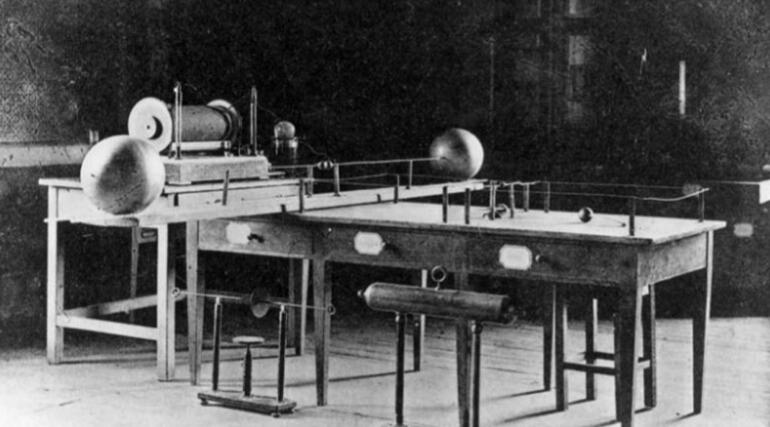
\includegraphics[height=2.40in,width=4.05in,viewport=0 0 580 325,clip]{Figures/Two-dark-cloud-in-physics-1.jpg}
\label{Classical_Mechanics}
\end{figure}
}

\frame
{
	\frametitle{\textrm{\small Newtonian, Lagrangian and Hamiltonian Mechanics}}
	\begin{itemize}
   		\setlength{\itemsep}{10pt}
		\item \textrm{\textcolor{blue}{Newtonian~Mechanics}}\\
		牛顿运动定律体系是以力、加速度、动量这些矢量为基本量来描述力学系统在欧氏空间的运动~(用几何方程表述约束)
	\item \textrm{\textcolor{blue}{Lagrangian~Mechanics}}\\
		拉格朗日力学是关于研究对象在其对应的约束系统下的运动形式,大大压缩牛顿方程描述需要的约束个数。不需要在另外设未知数目
	\item \textrm{\textcolor{blue}{Hamiltonian~Mechanics}}\\
		哈密度力学由拉格朗日力学演变而来,把位置和动量彻底分开,成为两种独立变量,由此诞生\textcolor{blue}{相空间}。把广义动量和广义坐标放在等同的位置上(正则配对,方程降阶)
		\vskip 6pt
		拉格朗日力学和哈密顿力学的基本量是\textcolor{blue}{系统的能量}等标量,通过变分原理建立系统的动力学方程,所以拉格朗日力学和哈密顿力学合称\textcolor{magenta}{分析力学}
	\end{itemize}
}

\frame
{
	\frametitle{相空间和时间平均}
	分子动力学模拟一般在相空间完成\\
	\vskip 3pt
	\textcolor{blue}{相空间}\textrm{(Phase~Space)}是表示系统所有可能所处状态的空间\\
	\vskip 5pt
{\fontsize{8.5pt}{6.2pt}\selectfont{
	\textcolor{blue}{系统中每个可能的状态在相空间中都存在一个确定的对应点}\\
	相空间是一个六维假想空间,其中\textcolor{blue}{动量}和\textcolor{blue}{空间}各占三维}}\\
	\vskip 8pt
	对于包含$N$个粒子的体系,构成$6N$维相空间$(\Gamma_N)$:~包括$3N$个空间$(\vec r)$自由度,$3N$个动量$(\vec p)$自由度
	\vskip 5pt
{\fontsize{8.2pt}{6.2pt}\selectfont{
	如果描述体系性质的状态函数$A$可以用空间和动量坐标表示~$A(\Gamma)$(如体系的总能或瞬时压力),其\textcolor{purple}{时间平均}值为}}
	\begin{displaymath}
		A_{\mathrm{obs}}=\langle A\rangle_{\mathrm{time}}=\langle A(\Gamma(t))\rangle_{\mathrm{time}}=\lim_{\tau\rightarrow\infty}\dfrac1{\tau}\int_{t=0}^{\tau}A(\Gamma(t))\mathrm{d}t
	\end{displaymath}
	\textcolor{magenta}{各态遍历假设}\textrm{(ergodic~hypothesis)}\\
	\vskip 5pt
{\fontsize{9.5pt}{6.2pt}\selectfont{
	只要演化时间足够长,孤立体系会\textcolor{red}{等概率地遍历每个可能的}微观状态~\\
换言之,\textcolor{blue}{体系足够长时间平均}等价于\textcolor{blue}{体系许可的大量系综的系综平均}
%分子动力学模拟的一个思想是用时间换取空间。我们无法得知系统在某一时刻所有可能的微观状态,但是可以通过一段时间的采样来获取系统大量的微观状态数。模拟的整个过程可以理解为建立了一个系综,而每一个时间点就是组成这个系综的一个系统,它们具有相同的限制条件(例如:粒子总数,温度、压强或体积等),但是具有不同的微观状态。系统的热力学量就是系综平均的结果。
}}
}

\frame
{
	\frametitle{分子动力学基本思想}
	\begin{itemize}
			\setlength{\itemsep}{3pt}
		\item 分子动力学模拟过程中产生的具体数据是\\
			\textcolor{blue}{粒子在相空间中随时间演化的 一系列点}
		\item 分子动力学模拟的直接结果是\\
			\textcolor{blue}{体系中全部粒子随时间变化的径迹\textrm{(trajectory)}}
		\item 体系的时间平均和其它物理性质都可以通过粒子径迹计算
		\item 约化单位\textrm{(reduced unit)}\\
{\fontsize{7.2pt}{6.2pt}\selectfont{
	数值模拟中使用的是内部单位,需要通过换算才能得到实际体系的真实物理单位(国际单位制,\textrm{Syst\`eme International $\mathrm{d}'$Unit\'es, SI})}}
	\begin{enumerate}
{\fontsize{7.2pt}{6.2pt}\selectfont{
		\item 四个基本物理量单位:\\
			长度\textrm{L}、质量\textrm{M}、时间\textrm{t},电荷电量\textrm{Q}
		\item 其它物理量:\\
			能量~$E=M\cdot L^2/t^2$\hskip 15pt温度~$T=E/k_{\mathrm{B}}$\hskip 15pt压力~$P=E/L^3$\\
			质量密度~$\rho=M/L^3$\hskip 8pt数量密度~$n=1/L^3$\hskip 8pt介电常数~$\varepsilon=\dfrac{N_{\mathrm{A}}\cdot Q^2}{L\cdot E}$
			\vskip 4pt
	这里$k_{\mathrm{B}}$是\textrm{Boltzmann}常数,$N_{\mathrm{A}}$是\textrm{Avogadro}常数}}
	\end{enumerate}
	\end{itemize}
}

\frame
{
	\frametitle{分子动力学基本思想}
	在相空间中,体系中粒子的运动由\textrm{Hamiltonian}方程描述
	\begin{displaymath}
		\begin{aligned}
			\dot{\vec r}_i=&\dfrac{\partial\mathbf{H}}{\partial\vec p_i}=\dfrac{\vec p_i}{m_i}\\
			\dot{\vec p}_i=&-\dfrac{\partial\mathbf{H}}{\partial\vec r_i}=\vec f_i
		\end{aligned}
	\end{displaymath}
	\textrm{Hamiltonian}$\mathbf{H}$的定义为
	\begin{displaymath}
		\begin{aligned}
			\mathbf{H}(\vec r,\vec p)=&\mathbf{K}(\vec p)+V(\vec r)\\
			\mathbf{K}(\vec p)=&\sum_i^N\dfrac{\vec p_i^2}{2m_i}
		\end{aligned}
	\end{displaymath}
	由此可得粒子运动遵守的\textrm{Newton}方程为
	\begin{displaymath}
		\begin{aligned}
			\dot{\vec x}=&\dfrac{\partial\mathbf{H}}{\partial\vec p_x}=\dfrac{\vec p_x}m=\vec v_x\\
			\dot{\vec p}_x=&-\dfrac{\partial\mathbf{H}}{\partial{\vec x}}=-\dfrac{\partial V(\vec x)}{\partial\vec x}=\vec F=m\vec a_x
		\end{aligned}
	\end{displaymath}
}

\frame
{
	\frametitle{分子动力学模拟流程}
\begin{figure}[h!]
\centering
\vspace{-10.0pt}
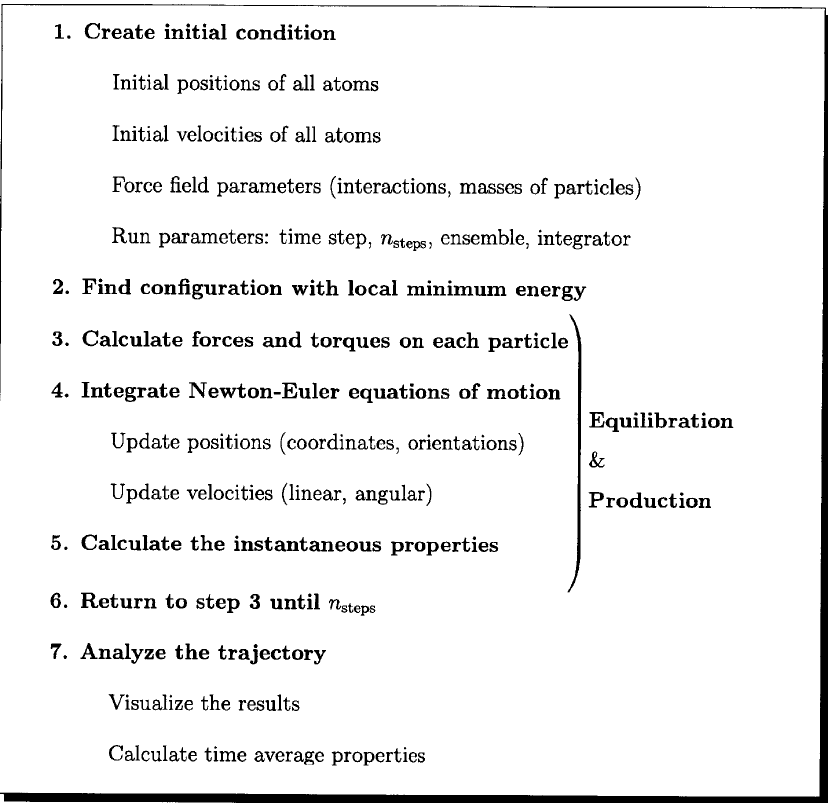
\includegraphics[height=2.70in,width=3.00in,viewport=30 20 750 794,clip]{Figures/The-molecular_dynamcis_algorithm.png}
\caption{\textrm{The steps in performing a molecular dynamcis simulation.}}
\label{The-molecular-dynamics_algorithm}
\end{figure}
}

\subsection{分子动力学的力场}
\frame[allowframebreaks]
{
	\frametitle{力场}
分子动力学中,粒子间相互作用用\textcolor{red}{力场}\textrm{(Force Field)},也就是“\textcolor{blue}{相互作用势}”,描述,力场的形式有很多种,一般将势函数分解为粒子间相互作用,包括双体相互作用、三体相互作用、$\cdots$
	\begin{displaymath}
		V(\vec r)=\sum_{ij}V_{ij}(\vec r_i,\vec r_j)+V_{ijk}(\vec r_i,\vec r_j,\vec r_k)+V_{ijkl}(\vec r_i,\vec r_j,\vec r_k,\vec r_l)+\cdots
	\end{displaymath}
\begin{figure}[h!]
\centering
\vspace{-18.0pt}
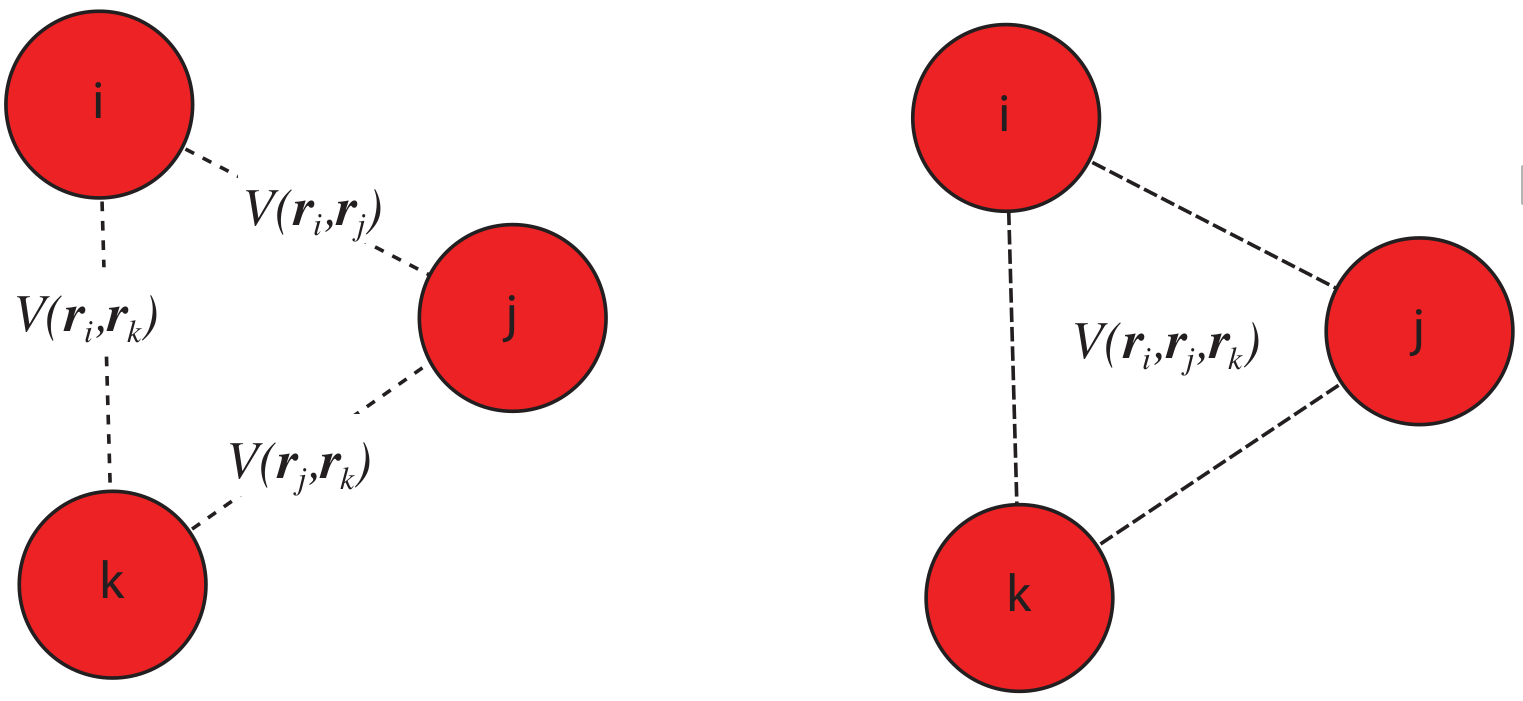
\includegraphics[height=1.47in,width=3.40in,viewport=0 0 1520 700,clip]{Figures/Interaction_particles.png}
\caption{\textrm{\tiny The Schematic representation of the interactions between pairs, triplets of particles.}}
\label{Interaction_particles}
\end{figure}

\begin{itemize}
			\setlength{\itemsep}{5pt}
	\item 一般说,力场中最主要来自双体相互作用(也称为``对势''),因此可将力场展开函数中的多体相互作用截断,仅保留双体相互作用的贡献
		\begin{displaymath}
			V(\vec r)=\sum_{ij}V_{ij}(\vec r_i,\vec r_j)
		\end{displaymath}
	\item 真实模拟中,为了更好地表示考虑粒子间相互作用的多体效应,双体相互作用用的是``有效对势'',有效对势包含了一部分粒子间的多体相互作用
		\begin{displaymath}
			V(\vec r)=\sum_{ij}V_{ij}^{\mathrm{eff}}(\vec r_i,\vec r_j)
		\end{displaymath}
	\item 具体计算使用的力场都是参数化的,这些参数主要通过对实验数据和结果的拟合确定
\end{itemize}

	典型力场的有
	\begin{itemize}
		\item \textrm{Lennard-Jones}对势和受力
	\begin{displaymath}
		\begin{aligned}
			U(r)=&4\varepsilon\bigg[\bigg(\dfrac{\sigma}{r}\bigg)^{12}-\bigg(\dfrac{\sigma}{r}\bigg)^6\bigg]\\ 
			\vec F(r)=&-\nabla V(r)=24\dfrac{\varepsilon}r\bigg[2\bigg(\dfrac{\sigma}{r}\bigg)^{12}-\bigg(\dfrac{\sigma}{r}\bigg)^6\bigg]\hat{\vec r}
		\end{aligned}
	\end{displaymath}
	{\fontsize{7.2pt}{6.2pt}\selectfont{这里$\varepsilon$和$\sigma$是和原子有关的参数}}
		\begin{itemize}{\fontsize{8.0pt}{6.2pt}\selectfont{
			\item \textcolor{blue}{$\dfrac1{r^6}$项}:~描述中性原子间的\textrm{Vander-der-Waals}的相互吸引作用(包含偶极-偶极相互作用)
			\item \textcolor{blue}{$\dfrac1{r^{12}}$项}:~描述电子云重叠引起的短程排斥作用
			\item \textrm{L-J}势能的最低点在$r_{\min}=2^{(1/6)}\sigma\approx1.122\sigma$\\
				$r<r_{\min}$时为排斥力,$r>r_{\min}$时为吸引力}}
		\end{itemize}
惰性气体的原子间相互作用仅用\textrm{L-J}基本可以完全描述
\begin{figure}[h!]
\centering
\vspace*{-0.15in}
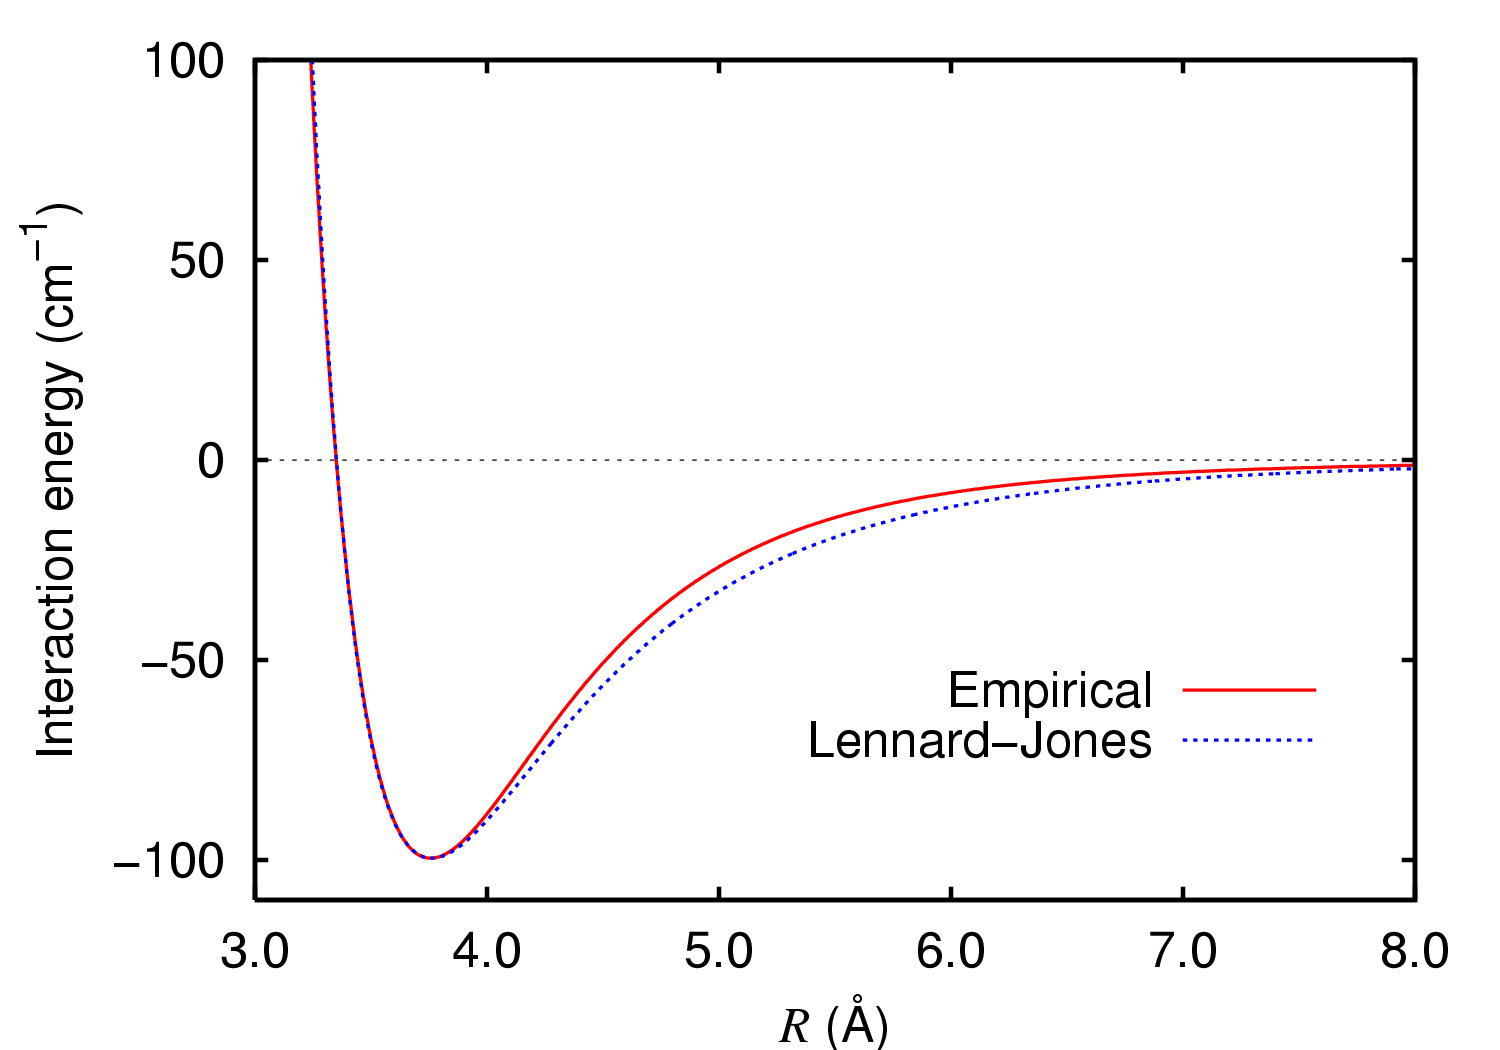
\includegraphics[height=2.05in,width=2.90in,viewport=0 0 350 270,clip]{Figures/Argon_dimer_potential_and_Lennard-Jones.png}
\caption{\tiny \textrm{The Lennard-Jones potential for argon dimer.}}%(与文献\cite{EPJB33-47_2003}图1对比)
\label{Potential-Lennard-Jones}
\end{figure}
%	由\textrm{L-J}势改造,可以得到\textrm{WCA}势和\textrm{PHS}势
\item \textrm{Morse}势
	\begin{displaymath}
		U(r)=-D_{\mathrm{e}}+D_{\mathrm{e}}\bigg(1-\mathrm{e}^{-a(r-r_{\mathrm{e}})}\bigg)^2
	\end{displaymath}
	{\fontsize{6.5pt}{6.2pt}\selectfont{这里$D_{\mathrm{e}}$是\textrm{Morse}势的势阱深,参数$a$确定势阱宽度,$r_{\mathrm{e}}$是原子处于平衡位置的平衡键长 }}
\begin{figure}[h!]
\centering
\vspace*{-0.10in}
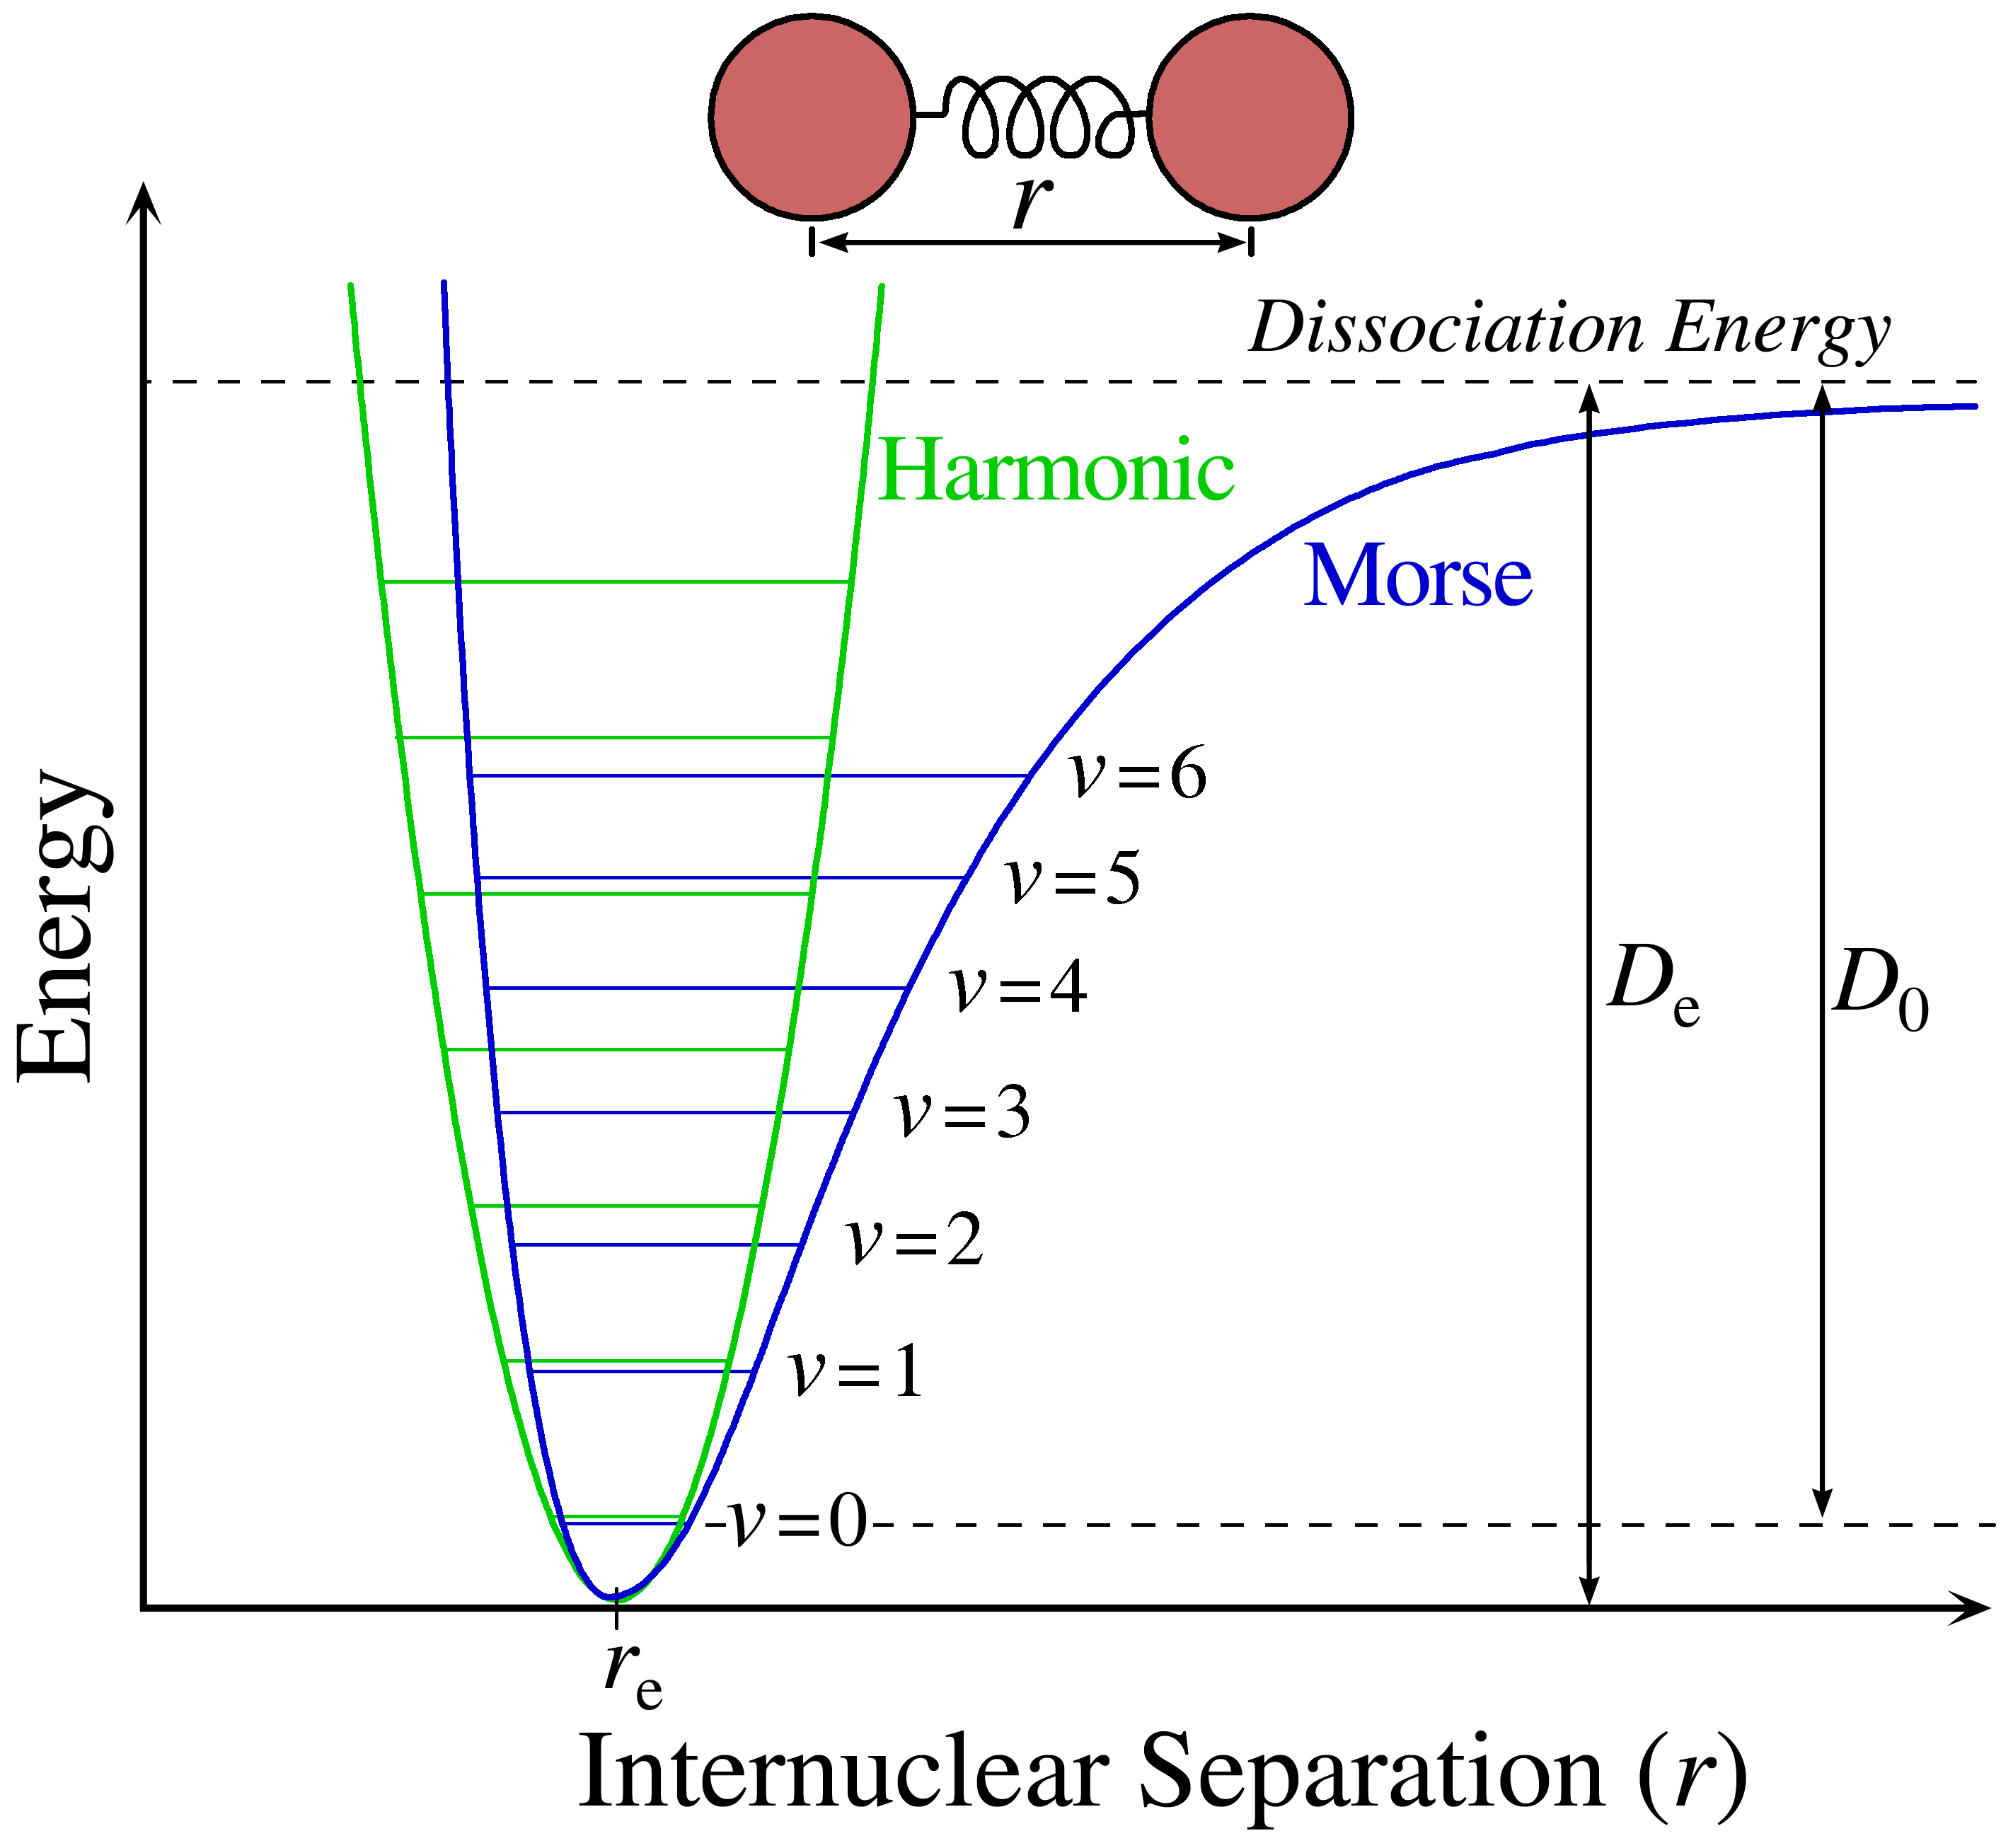
\includegraphics[height=1.35in,width=1.95in,viewport=0 0 3540 2770,clip]{Figures/Morse-potential.png}
\caption{\tiny \textrm{The Morse potential (blue) and harmonic oscillator potential (green).}}%(与文献\cite{EPJB33-47_2003}图1对比)
\label{Potential-Morse}
\end{figure}
\item \textrm{EAM}势\\
	{\fontsize{7.2pt}{6.2pt}\selectfont{对于金属晶体,内能虽可以表示为对相互作用之和,但拟合原子受力非常困难\footnote{\fontsize{5.2pt}{3.2pt}\selectfont{应用二体势计算金属弹性常数时必须涉及对体积很敏感的能量项,因为涉及缺陷、表面的体积很难确定。}}:\\
	\textcolor{red}{从物理上说金属原子处于电子海洋中,电子密度来自多个原子的贡献,这是自由电子气带来的多体效应}}}\\
	\textrm{EAM}将金属中原子的势能表示为二体势和多体势之和
	\begin{displaymath}
		E_i=F_{\alpha}\bigg(\sum_{j\neq i}\rho_{\beta}(r_{ij})\bigg)+\dfrac12\sum_{j\neq i}\phi_{\alpha\beta}(\vec r_{ij})
	\end{displaymath}
	{\fontsize{7.2pt}{6.2pt}\selectfont{$\alpha$和$\beta$分别为位置$i$、$j$处的原子类型\\
		$\phi$是二体势,是原子$\alpha$和$\beta$和原子间距$r_{ij}$的函数\\
		$F$是多体势,是其余原子在位置$i$处的电荷密度与位置$i$处原子$\alpha$的相互作用能,由原子类型$\alpha$和位置$i$处的电子密度确定\\
		位置$j$原子在位置$i$处产生的电荷密度$\rho$只与位置$j$处原子类型$\beta$和原子间距$r_{ij}$有关,与方向无关
	}}\\
	各类\textrm{EAM}势中,$\phi(r)$、$\rho(r)$和$F(\rho)$都不是解析的,以数值形式存储
	\end{itemize}
}

\frame
{
	\frametitle{复杂研究对象中的力场}
\begin{figure}[h!]
\centering
\vspace*{-0.10in}
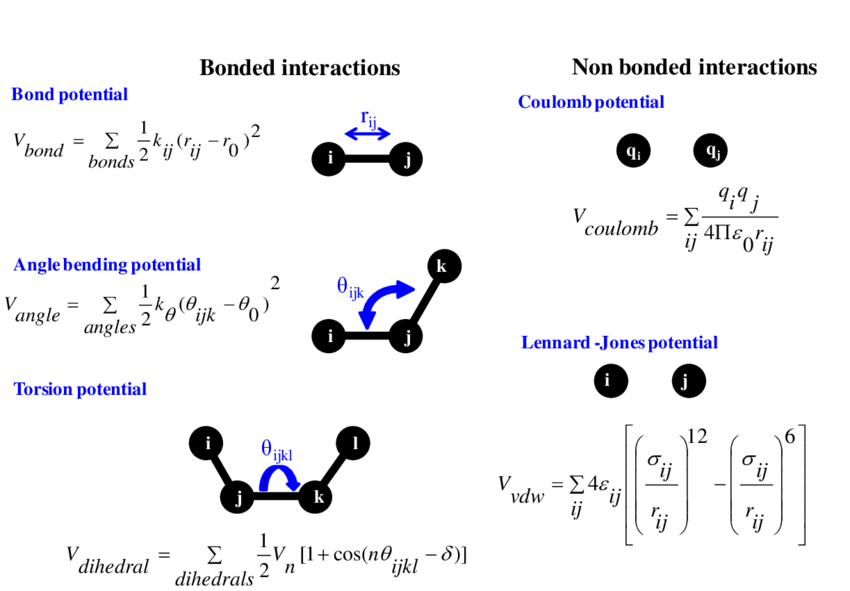
\includegraphics[height=2.70in,width=3.95in,viewport=0 0 830 550,clip]{Figures/Bonded-and-non-bonded-interactions-used-to-describe-interactions-between-atoms.png}
%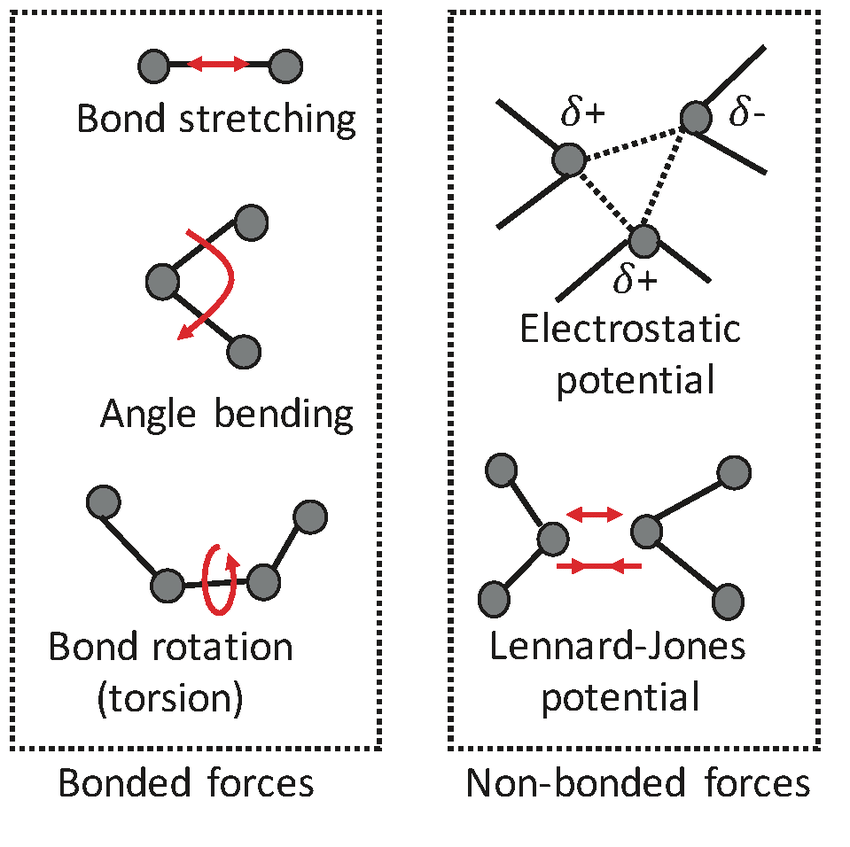
\includegraphics[height=2.70in,width=2.85in,viewport=0 40 830 850,clip]{Figures/Bonded-and-non-bonded-forces-consider-in-MD-simulations.png}
\caption{\tiny \textrm{Bonded and non-bonded forces consider in MD simulations.}}%(与文献\cite{EPJB33-47_2003}图1对比)
\label{Bond-non-Bonded}
\end{figure}
}

\frame
{
	\frametitle{复杂研究对象中的力场}
\begin{figure}[h!]
\centering
\vspace*{-0.15in}
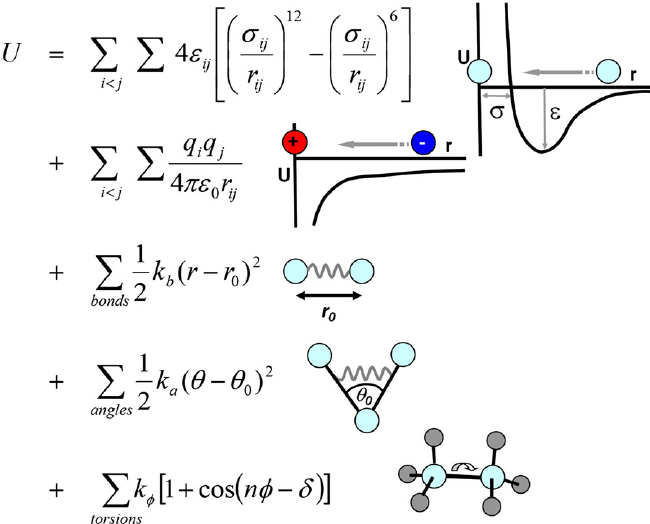
\includegraphics[height=2.75in,width=3.55in,viewport=0 0 660 540,clip]{Figures/Potential-energy-function-for-molecular-interactions-in-the-molecular-mechanics.png}
\caption{\tiny \textrm{Potential energy function for molecular interactions in the molecular mechanics.}}%(与文献\cite{EPJB33-47_2003}图1对比)
\label{Potential-component}
\end{figure}
}

\subsection{分子动力学{\rm Verlet}算法}
\frame
{
	\frametitle{分子的受力与运动}
	装有$N$个经典粒子的$L_1\times L_2\times L_3$容器内,假设粒子间只有简单的二体相互作用%\footnote{\fontsize{7.2pt}{6.2pt}\selectfont{二体作用是粒子间多体相互作用的简化,只考虑粒子两两间彼此相互作用。}}
	$\vec F(r)$,力的大小仅与粒子间间距$r$相关
	\begin{displaymath}
		\vec F(R_i)=\sum_{\substack{j=1\\j\neq i}}^N F(|\vec r_i-\vec r_j|)\hat{\vec r}_{ij}
	\end{displaymath}
	{\fontsize{7.2pt}{6.2pt}\selectfont{这里$R$代表全部原子坐标$\vec r_i$,$\hat{\vec r}_{ij}$是表示粒子$i$指向粒子$j$的矢量($\vec r_j-\vec r_i$)的单位矢量}}

	在经典力学框架下,粒子$i$的受力运动方程是:~
	\begin{displaymath}
		\dfrac{\mathrm{d}^2\vec r_i(t)}{\mathrm{d}t^2}=\dfrac{\vec F_i(R)}{m_i}
	\end{displaymath}
	粒子$i$的质量是$m_i$\\
	\textcolor{purple}{经典分子动力学,就是应用数值模拟对大量粒子求解该方程,基于统计力学原理,研究物质的状态和热力学性质}
}

\frame
{
	\frametitle{经典分子动力学与\textrm{Verlet}算法}
	分子动力学模拟研究的对象是平衡态体系
	\begin{itemize}
		\item 初始化
		\item 开始分子运动模拟,直到模拟体系达到平衡
		\item 继续模拟体系的物理性质,保存计算结果
	\end{itemize}
	\textcolor{blue}{标准\textrm{Verlet}算法:~}求解作用力$\vec F$下单个粒子运动的积分
	\begin{displaymath}
		\vec r(t+h)=2\vec r(t)-\vec r(t-h)+h^2\vec F(\vec r(t))/m
	\end{displaymath}
	{\fontsize{7.2pt}{6.2pt}\selectfont{这里$h$是时间步长,$t=nh$是模拟累积时间,$\vec r(t)$是粒子在时间$t$时的位置\\
	\textcolor{magenta}{每个时间步长的误差为$h^4$,在模拟时间范围内的累积误差是$h^2$}
\vskip 5pt
	{\fontsize{7.2pt}{6.2pt}\selectfont{如果已知模拟粒子的初始速度$\vec v$和时间,取初始态时间$t=0$}}
	\begin{displaymath}
		\vec r(h)=\vec r(0)=h\vec v(0)+\dfrac{h^2}2\vec F[\vec r(t=0)]~\qquad~ (m\equiv1)
	\end{displaymath}
误差为$h^3$,速度随时间变化的函数
\begin{displaymath}
	\vec v(t)=\dfrac{\vec r(t+h)-\vec r(t-h)}{2h}+\mathscr{O}(h^2)
\end{displaymath}
}}
}

\frame
{
	\frametitle{经典分子动力学与\textrm{Verlet}算法}
	\textrm{Verlet}算法有两种被普遍应用的变体形式,相比于标准\textrm{Verlet}算法,这两种方法误差累积效应更小
	\begin{itemize}
		\item \textcolor{blue}{蛙跳(\textrm{Leap-Frog})法}
			\begin{displaymath}
				\begin{aligned}
					\vec v(t+h/2)=&\vec v(t-h/2)+h\vec F[\vec r(t)]\\
					\vec r(t+h)=&\vec r(t)+h\vec v(t+h/2)
				\end{aligned}
			\end{displaymath}
		\item \textcolor{blue}{速度-\textrm{Verlet}算法}
			\begin{displaymath}
				\vec v(t)=\dfrac{\vec r(t+h)-\vec r(t-h)}{2h}
			\end{displaymath}
			\begin{displaymath}
				\begin{aligned}
					\vec r(t+h)=&\vec r(t)+h\vec v(t)+h^2\vec F(t)/2\\
					\vec v(r+h)=&\vec v(t)+h[\vec F(t+h)+\vec F(t)]/2
				\end{aligned}
			\end{displaymath}
			速度-\textrm{Verlet}算法更稳定也更方便,但需要保存$\vec F(t)$和$\vec F(t+h)$两个力的数组
	\end{itemize}
}

\frame
{
	\frametitle{经典分子动力学与\textrm{Verlet}算法}
	以下算法与速度-\textrm{Verlet}算法完全等价,但只需要保留$\vec F(t)$一个数组
	\begin{displaymath}
		\begin{aligned}
			\tilde{\vec v}(t)=&\vec v(t)+h\vec F(t)/2\\
			\vec r(t+h)=&\vec r(t)+h\tilde{\vec v}(t)\\
			\vec v(t+h)=&\tilde{\vec v}(t)+h\vec F(t+h)/2
		\end{aligned}
	\end{displaymath}
	而粒子受力$\vec F(t+h)$则在第二步、第三步之间临时计算
\vskip 5pt
	{\fontsize{6.2pt}{4.2pt}\selectfont{一般地,作用在粒子$i$上的力,是所有与粒子$i$的相互作用的“合成”结果
	\begin{displaymath}
		\vec F_i(R)=-\dfrac{\partial U(\{\vec r_i\})}{\partial \vec r_i}
	\end{displaymath}
	通常总的势能$U(\{\vec r_i\})$拆解为各部分贡献
	\begin{displaymath}
		U(\{\vec r_i\})=\sum_iU_1(\vec r_i)+\sum_i\sum_{j>i}U_2(\vec r_i,\vec r_j)+\sum_i\sum_{j>i}\sum_{k>j}U_3(\vec r_i,\vec r_j,\vec r_k)+\cdots
	\end{displaymath}
	这里$U_1(\vec r_i)$是单体势,一般是单个粒子在外场(如重力场、电场)中的势能,与材料性质无关\\
$U_2(\vec r_i,\vec r_j)$是双体势,$U_3(\vec r_i,\vec r_j,\vec r_k)$是描述粒子间对相互作用的主要函数}}

	在分子动力学计算中,力的计算需要更多的时间,因为其计算耗时步数是$\mathscr{O}(N^2)$,\textcolor{blue}{对于周期体系,这种力的计算尤其需要谨慎}
}

\subsection{平衡态统计基础}
%\frame
%{
%	\frametitle{开始统计力学}
%	\textrm{No other textbook, and possibly no other book, will ever have a better opening paragraph than Goodstein's "States of Matter"}:
%\begin{figure}[h!]
%\centering
%\vspace*{-0.03in}
%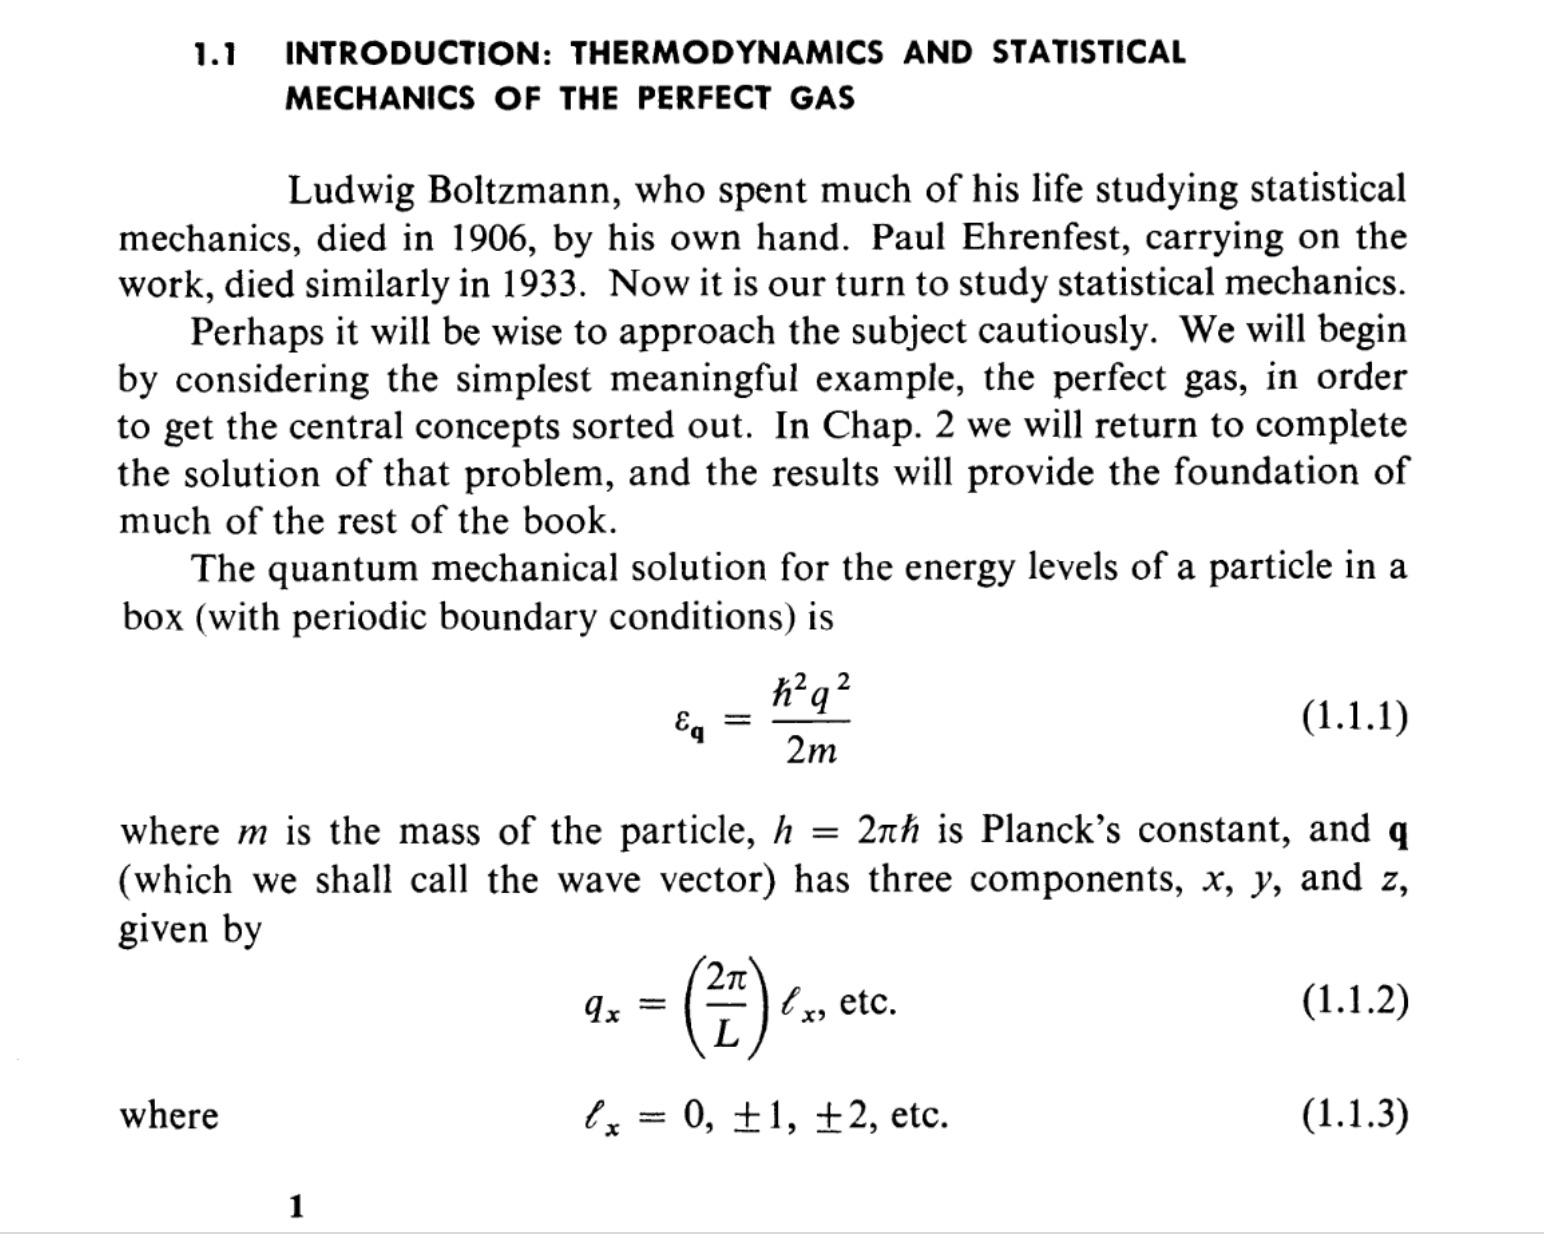
\includegraphics[height=2.25in,width=3.25in,viewport=0 0 1560 1240,clip]{Figures/Statistical-mechanics_suicide.png}
%%\caption{\fontsize{5.2pt}{1.2pt}\selectfont{\textrm{David~L.~Goodstein, \textit{States~of~Matter}, Dover Publication, Inc, Mineola, New York, (1975)}}}%(与文献\cite{EPJB33-47_2003}图1对比)
%\caption{\fontsize{4.2pt}{1.2pt}\selectfont{\textrm{David~L.~Goodstein, \textit{States~of~Matter}, Prentice-Hall, Inc, Englewood Cliffs, New Jersey, (1975)}}}%(与文献\cite{EPJB33-47_2003}图1对比)
%\label{Statistical_Mechanics-suicide}
%\end{figure}
%}
%
\frame
{
	\frametitle{平衡态统计基础}
	系综(\textrm{Ensembles})是在一定的宏观条件下,由大量微观粒子组成的性质和结构完全相同的、处于各种运动状态的、各自独立的系统整体的集合。简言之,系综是给定宏观条件下,所有微观状态的集合。
%	应用\textrm{Verlet}算法,完成单粒子运动的数值积分,可以得到动力学体系的\textrm{Hamiltonian}对应的能量,进而应用统计力学的统计系综,获得宏观体系的物理量
	\vskip 3pt
	\textcolor{blue}{等概率原理}\textrm{(Principle of equal weights)}:\\
	一个热力学体系有相同的概率到达每个可能经历的微观态。\\
	等概率原理导出\textrm{Boltzmann}分布
	\begin{displaymath}
		P_j=\dfrac{\mathrm{e}^{-\beta\varepsilon_j}}Q
	\end{displaymath}
	这里$Q$称为配分函数\textrm{(partition function)}
	\begin{displaymath}
		\begin{aligned}
			Q=&\sum_i\mathrm{e}^{(-\beta\varepsilon_i)}\\
			\beta=&1/k_{\mathrm{B}}T
		\end{aligned}
	\end{displaymath}
	物理量的系综平均
	\begin{displaymath}
		\langle A\rangle=\sum_jA_j\mathrm{e}^{(-\beta\varepsilon_j)}/Q
	\end{displaymath}
}

\frame
{
	\frametitle{常用统计系综}
\begin{figure}[h!]
\centering
\vspace*{-0.20in}
%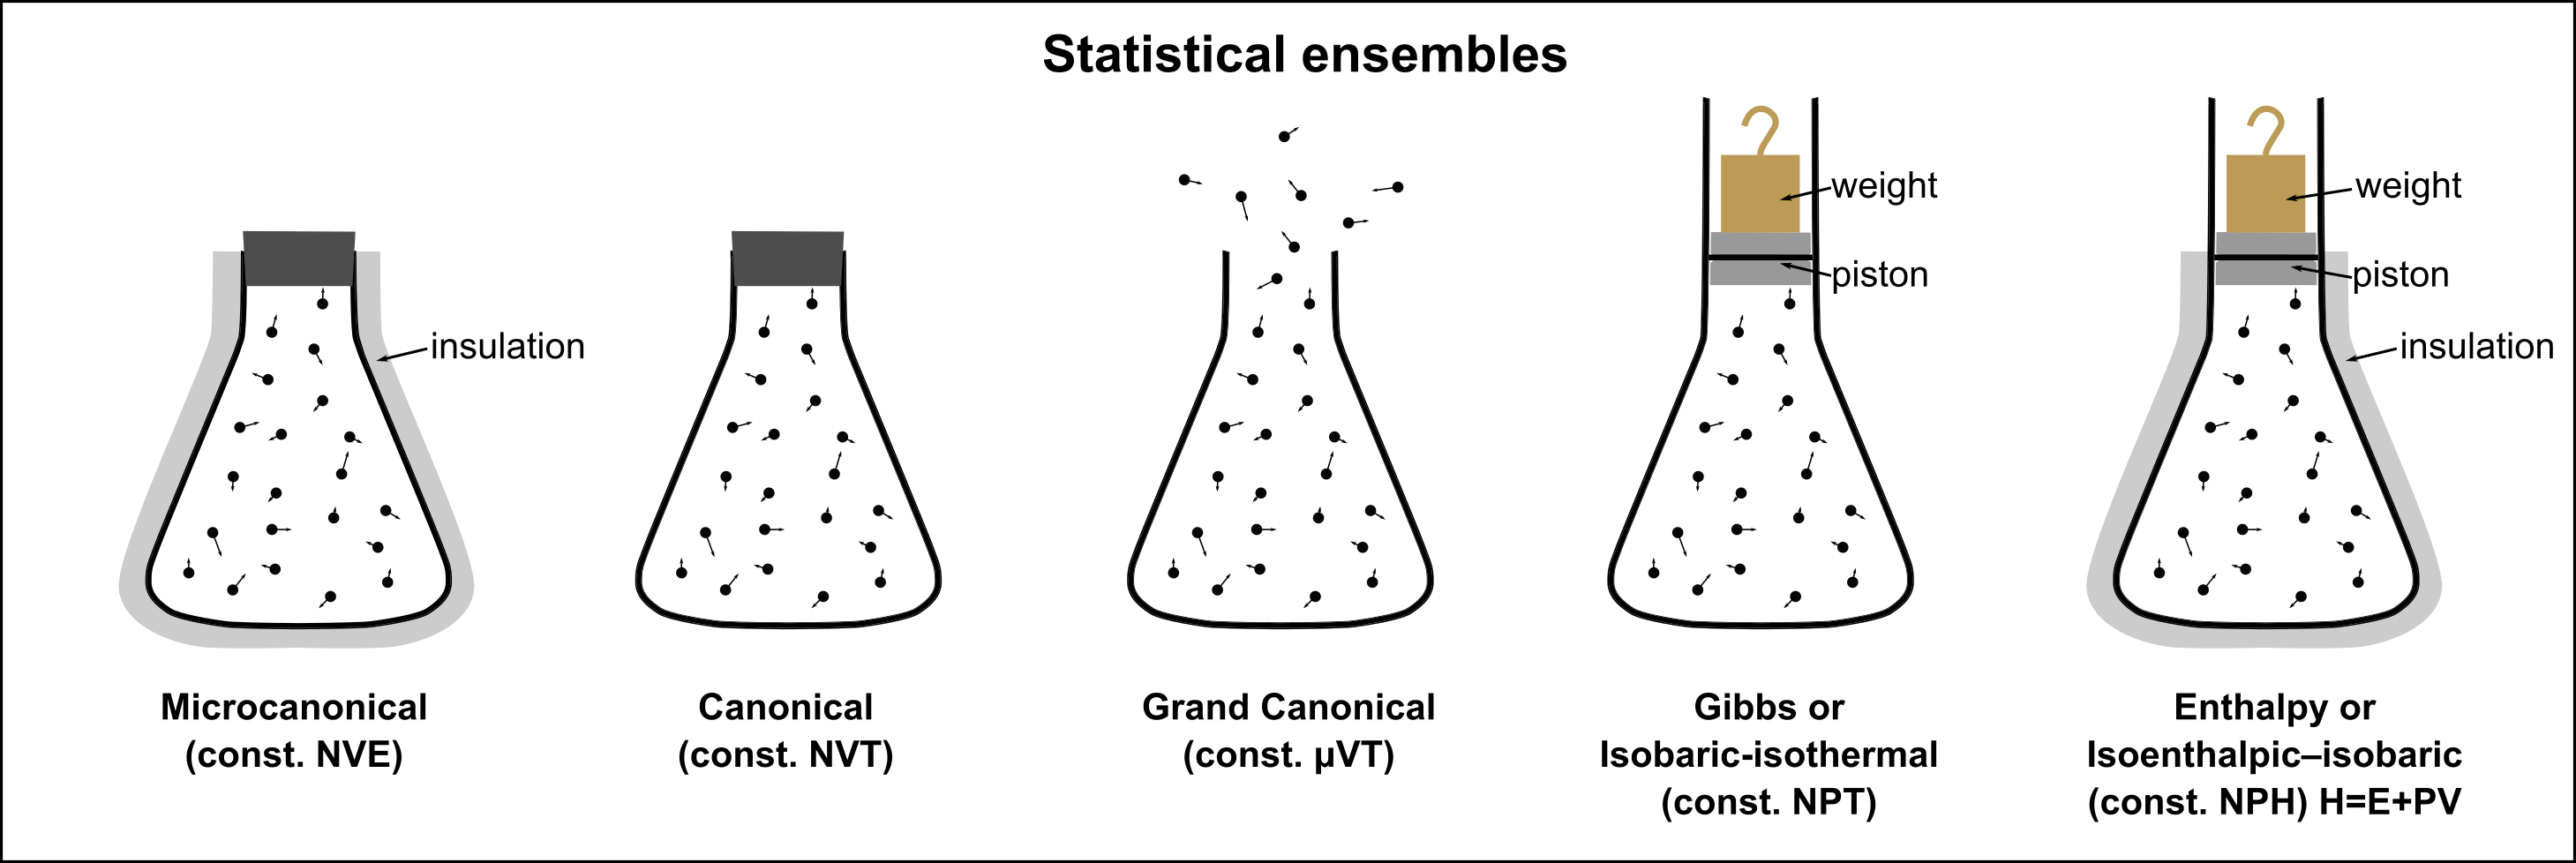
\includegraphics[height=1.60in,width=3.85in,viewport=0 0 1420 570,clip]{Figures/Statistical_Ensembles.png}
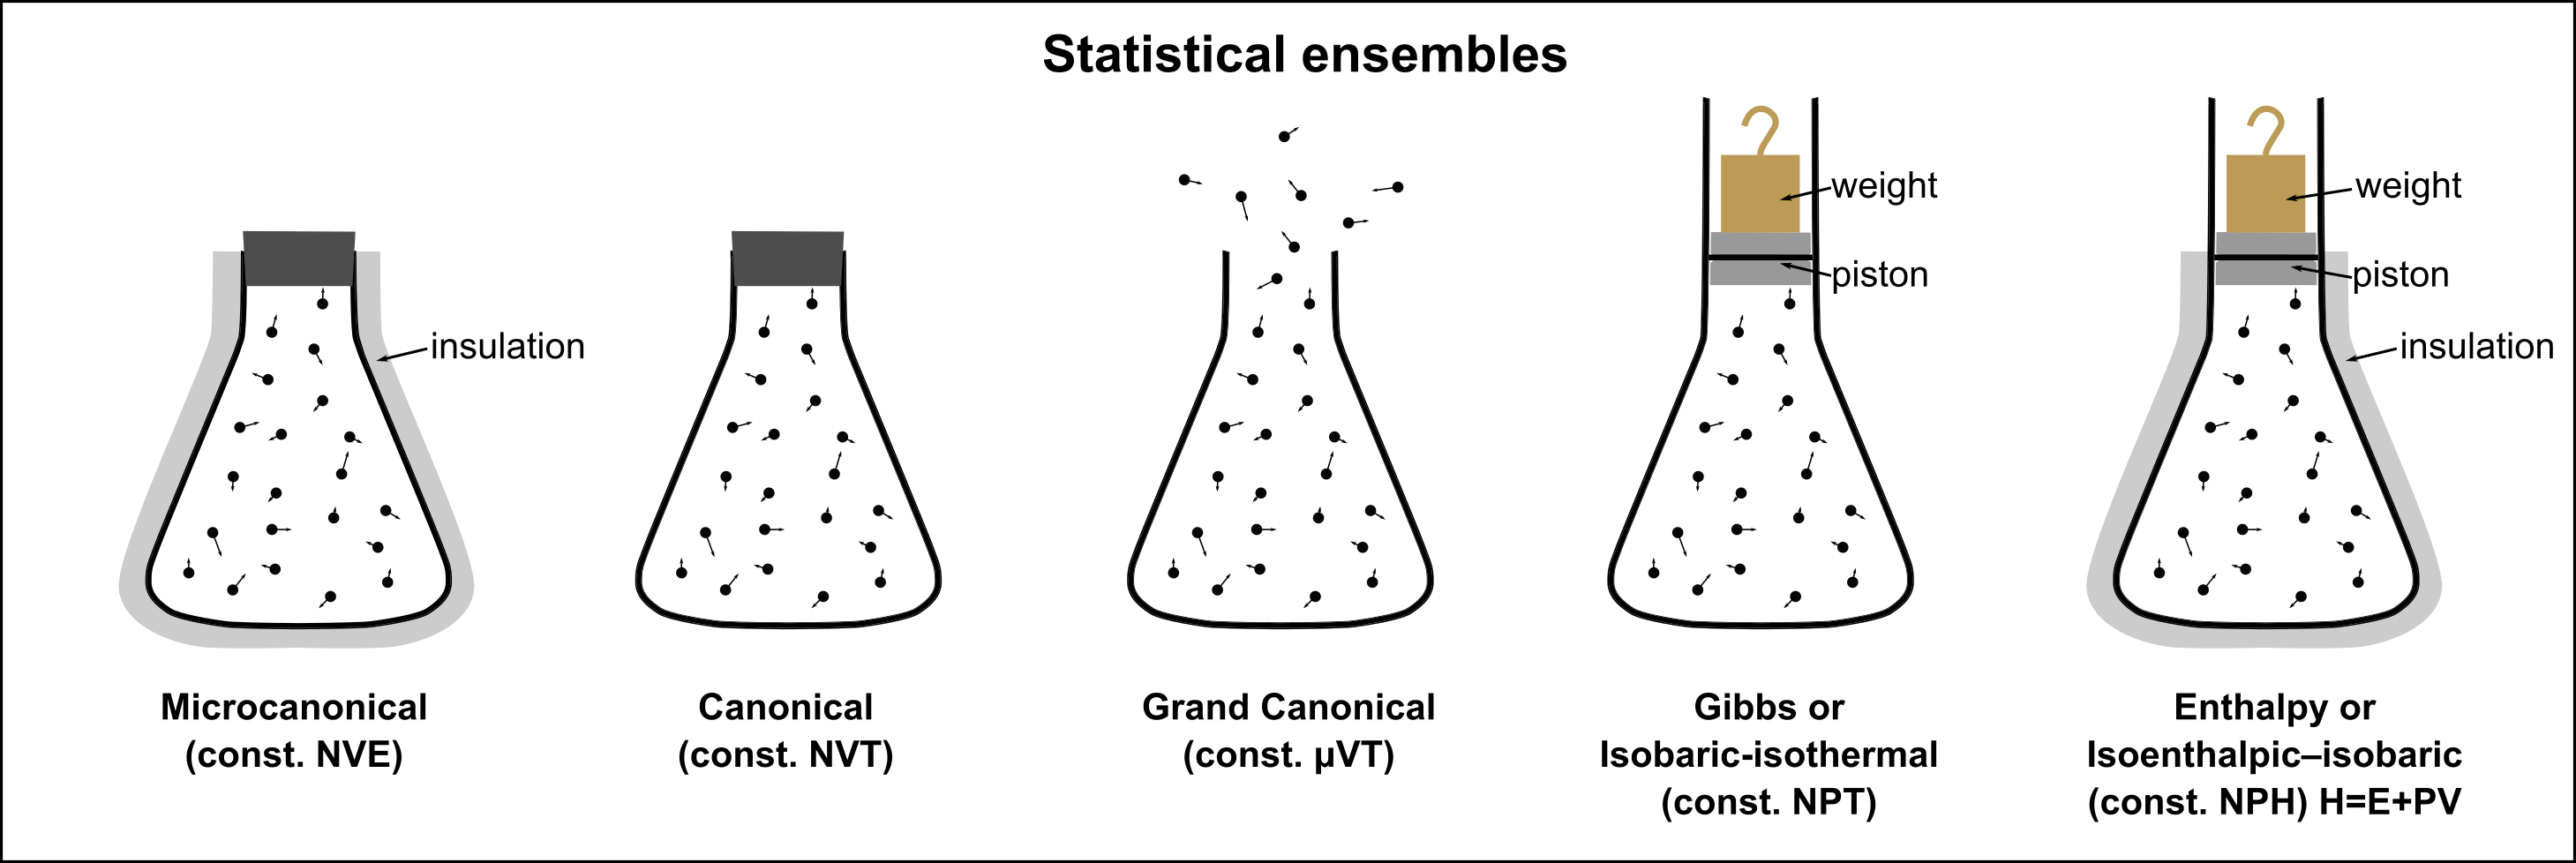
\includegraphics[height=1.20in,width=3.75in,viewport=0 0 1420 470,clip]{Figures/Statistical_Ensembles.png}
\caption{\tiny \textrm{The Statistical Ensembles.}}%(与文献\cite{EPJB33-47_2003}图1对比)
\label{Statistical_Ensembles}
\end{figure}
\vskip -15pt
\begin{itemize}
		{\fontsize{7.2pt}{1.2pt}\selectfont{
		\item 微正则系综\textrm{(Mircocanonical Ensemble)}%\footnote{\fontsize{4.5pt}{1.2pt}\selectfont{\textrm{canonical},汉译作``正则'',出自《楚辞\textperiodcentered 离骚》``皇揽揆余於初度兮,肇锡余以嘉名;~名余曰\textcolor{red}{正则}兮,字余曰灵均'',《楚辞章句》\upcite{Chucizhangju}:~``正,平也;~则,法也;~灵,神也;~均,调也。言正平可法则者,莫过于天;~养物均调者,莫神于地。高平曰原,故父伯庸名我为平以法天,字我为原以法地。言己上之能安君,下之能养民也。''意思是说``正则''、``灵均''隐喻着某种意义,即平正是天的象征,原均是地的象征。因此正则的含义是``\textcolor{blue}{符合天道}'',与\textrm{canonical}的意思\textrm{of, relating to, or forming a canon}意义一致。}}
			:~\textrm{NVE}皆为常数
		\item 正则系综\textrm{(Canonical Ensemble)}:~\textrm{NVT}皆为常数
		\item 巨正则系综\textrm{(Grandcanonical Ensemble)}:~\textrm{$\mu$VT}皆为常数,粒子数不固定
		\item 等压-等温系综\textrm{(Isobaric-Isothermal Ensemble)}:~\textrm{NPT}皆为常数
		\item 等焓-等压系综\textrm{(Isoenthalpic-Isobaric Ensemble)}:~\textrm{NPH}皆为常数
		\item 等张力-等温系综\textrm{(Isotension-Isothermal Ensemble)}:~容器形状可变 }}
\end{itemize}
}

\frame
{
	\frametitle{常用热力学量}
	\begin{itemize}
{\fontsize{7.8pt}{1.2pt}\selectfont{
		\item 动能 ~$E_{\mathrm{k}}=\bigg\langle\sum\limits_{i=1}^N\dfrac12m_iv_i^2\bigg\rangle$
		\item 势能 ~$E_{\mathrm{p}}=\bigg\langle\sum\limits_{i=1}^NE_{\mathrm{p}i}\bigg\rangle$
		\item 温度 ~$T=\dfrac1{\mathrm{d}Nk_{\mathrm{B}}}\bigg\langle\sum\limits_{i=1}^Nm_iv_i^2\bigg\rangle$ ~~~~ 其中$\mathrm{d}$是空间维度
		\item 压强 ~$p=\dfrac{k_{\mathrm{B}}TN}{V}+\dfrac1{\mathrm{d}V}\bigg\langle\sum\limits_{i<j}\vec f_{ij}\cdot\vec r_{ij}\bigg\rangle$
		\item 焓 ~$H=E+pV$ ~~~~ 相当于\textrm{NPT}下的有效总内能
		\item 熵 ~$S=k_{\mathrm{B}}\ln\Omega(N,V,E)$ ~~~~ $\Omega$是系统的总的微观状态数
		\item \textrm{Helmholtz}自由能:~\textcolor{blue}{\textrm{NVT}下的自由能}
			\begin{displaymath}
				F=E-TS=-k_{\mathrm{B}}T\ln{Q}
			\end{displaymath}
		\item \textrm{Gibbs}自由能:~\textcolor{blue}{\textrm{NPT}下的自由能}
			\begin{displaymath}
				G=F+pV=E-TS+pV
			\end{displaymath}
		\item 化学势 ~$\mu=\dfrac{\partial G}{\partial N}\bigg|_{T,p}=\dfrac{\partial F}{\partial N}\bigg|_{T,V}$}}
	\end{itemize}
}

\subsection{采样与模拟}
\frame
{
	\frametitle{空间、边界与周期边界条件}
	\begin{itemize}
		\item 空间的连续性
			\vskip 2pt
			{\fontsize{8.5pt}{1.2pt}\selectfont{离散模型:~如\textrm{Ising}模型\\
			连续模型 }}
		\item 边界条件:~自由、刚性、周期
	\end{itemize}
	\textcolor{blue}{周期边界条件}\textrm{(Periodic Boundary Condition, PBC)}\\
	\begin{itemize}
		\item \textcolor{blue}{目标}:~少量分子或团簇$(10^3\sim10^6)$的模拟与含有大量宏观粒子体系$(\sim10^{23})$
		\item \textcolor{blue}{策略}:~模拟的容器中粒子与无穷多镜像中粒子存在相互作用
	\end{itemize}
	\begin{displaymath}
		\begin{aligned}
			\vec F_{\mathrm{PBC}}(\vec r_i-\vec r_j)=&\sum_n\vec F\bigg(\bigg|\vec r_i-\vec r_j+\sum_{\mu=1}^3\mathbf{L}_{\mu}n_{\mu}\bigg|\bigg)\\
			E_{\mathrm{tot}}=&\dfrac12\sideset{}{^{\prime}}\sum_{i,j,n}\varepsilon\big(\big|\vec r_{ij}+n\mathbf{L}\big|\big)
		\end{aligned}
	\end{displaymath}
}

\frame
{
	\frametitle{空间、边界与周期边界条件}
\begin{figure}[h!]
\centering
\vspace*{-0.15in}
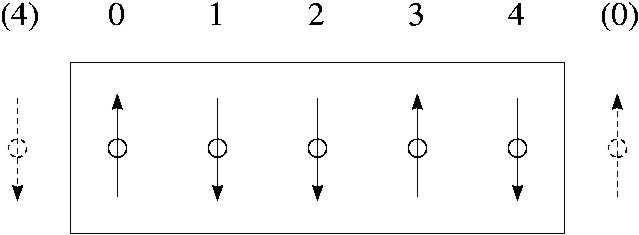
\includegraphics[height=0.75in,width=2.35in,viewport=0 0 460 170,clip]{Figures/Periodic-boundary-conditions-on-a-spin-lattice.jpg}
\vskip 1pt
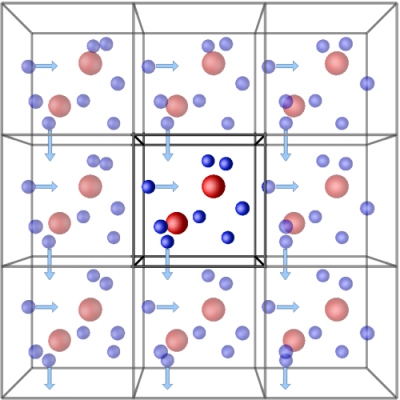
\includegraphics[height=1.95in,width=2.15in,viewport=0 0 300 300,clip]{Figures/Periodic-boundary-conditions.png}
\caption{\tiny \textrm{Schematic representation of the idea of periodic boundary conditions.}}%(与文献\cite{EPJB33-47_2003}图1对比)
\label{Periodic_boundary_conditions}
\end{figure}
}

\frame
{
	\frametitle{模拟与采样参数}
	\begin{itemize}
		\item \textcolor{blue}{特征长度}\textrm{(characteristic length)}:~物理量在空间的相关长度\\
			{\fontsize{8.5pt}{1.2pt}\selectfont{原则上,模拟容器的边长应大于关心物理量的特征长度;~具体操作上,可以通过变化模拟尺寸来了解有限尺寸效应\textrm{(finite size effect)}的影响}}
		\item \textcolor{blue}{截断距离}\textrm{(cutoff distance)}:~应小于模拟容器边长的一半\\
			{\fontsize{8.5pt}{1.2pt}\selectfont{避免同一粒子与两个镜像同时作用;~截断的处理方式有:~简单截断、截断平移、最小镜像法等三种}}
		\item \textcolor{blue}{采样}\textrm{(sampling)}:~本质是有限时间内的重要性采样\textrm{(importance sampling)}\\
			{\fontsize{8.5pt}{1.2pt}\selectfont{采样对系综平均贡献最大的瞬时量的子集,一般采用均匀时间间隔采样}}
		\item \textcolor{blue}{初始构型}\textrm{(Initial Configuration)}:~要尽量接近平衡态\\
			{\fontsize{8.5pt}{1.2pt}\selectfont{一般需要一定的初始模拟过程使得初始构型达到平衡态,在此初始模拟过程中不采样,需要根据某些参数的变化观察系统是否达到平衡态(液体体积很容易平衡,势能次之,扩散系数较难达到平衡)}}
		\item \textcolor{blue}{样本相关度}\textrm{(Correlation)}:~离得越近采样样本相关度越大\\
			{\fontsize{8.5pt}{1.2pt}\selectfont{相关的样本不影响平均值,但会影响误差范围}}
	\end{itemize}
}

\frame
{
	\frametitle{\textrm{Maxwell-Boltzmann}分布}
\begin{figure}[h!]
\centering
\vspace*{-0.15in}
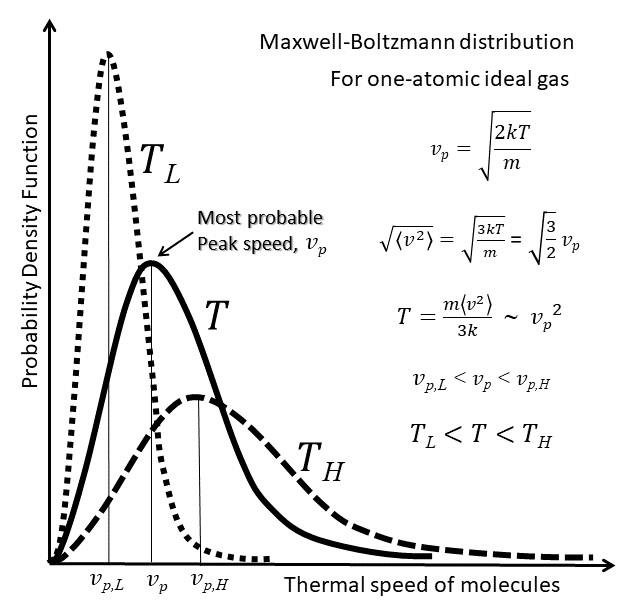
\includegraphics[height=2.75in,width=3.25in,viewport=0 0 470 460,clip]{Figures/Maxwell-Boltzmann-distribution-Energetic-molecules-of-an-ideal-gas.jpeg}
%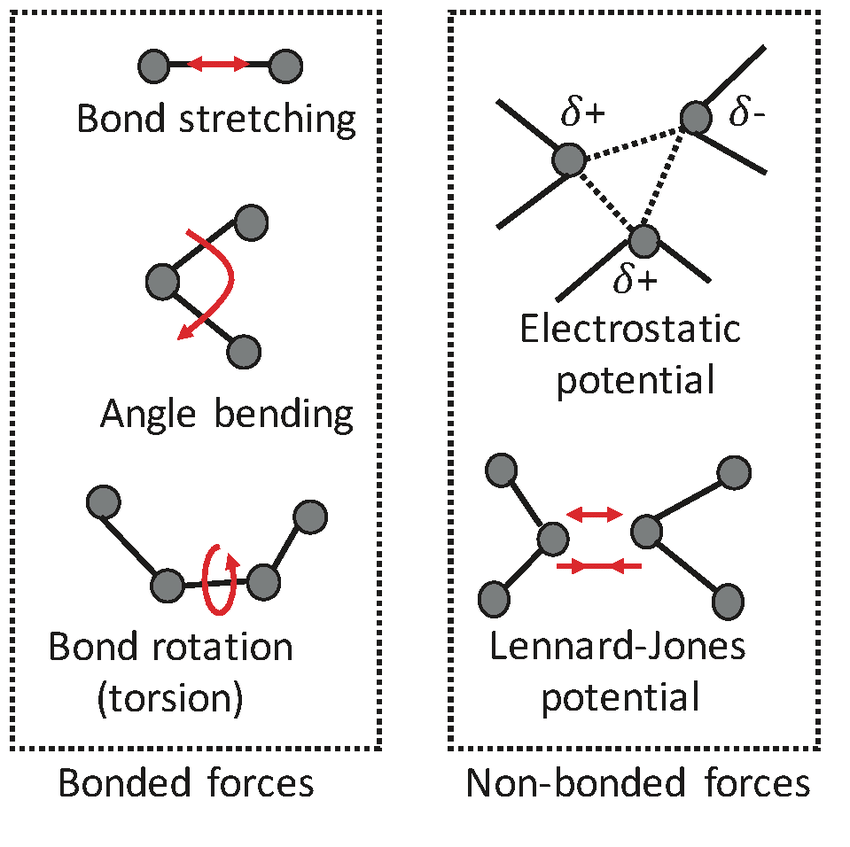
\includegraphics[height=2.70in,width=2.85in,viewport=0 40 830 850,clip]{Figures/Bonded-and-non-bonded-forces-consider-in-MD-simulations.png}
\caption{\tiny \textrm{Maxwell-Boltzmann distribution Energetic molecules of an ideal gas.}}%(与文献\cite{EPJB33-47_2003}图1对比)
\label{Maxwell-Boltzmann-distribution}
\end{figure}
}

\frame
{
	\frametitle{热耦或热浴\textrm{(Thermostat or Heat~Bath)}}
	\begin{itemize}
		\item \textrm{Isokinetics thermostat}:\\
			每一步采样都对速度进行修正,直到体系达到设定的目标温度
			\begin{displaymath}
				\dfrac32Nk_{\mathrm{B}}T=\dfrac12\sum_im_iv_i^2\Longrightarrow v_i^{\mathrm{scale}}=\lambda v_i\quad\mbox{有}~\lambda=\sqrt{\dfrac{T}{T_0}}
			\end{displaymath}
		\item \textrm{Berendsen thermostat}:
			\begin{displaymath}
				\lambda=\bigg[1+\dfrac{\Delta t}{\tau_T}\bigg(\dfrac{T}{T_0}-1\bigg)\bigg]^{\frac12}
			\end{displaymath}
		\item \textrm{Andersen thermostat}:\\
			每一步从温度为$T$的\textrm{Maxwell-Boltzmann}分布中随机产生一个速度赋予被选中的粒子
		\item \textrm{Nos\'e-Hoover thermostat}:\\
			增加额外的自由度,在扩展的微正则系综内实现实际体系的正则系综
	\end{itemize}
}

\frame
{
	\frametitle{离子间相互作用的\textrm{Ewald}求和}
	周期边界下长程\textrm{Coulomb}相互作用的计算\\
	通过屏蔽电荷将点电荷分解为时空间中的长程部分和短程部分
	\begin{itemize}
		\item \textcolor{blue}{短程部分}:~实空间截断
		\item \textcolor{blue}{长程部分}:~$\vec k$-空间截断
	\end{itemize}
\begin{figure}[h!]
\centering
%\vspace*{-0.20in}
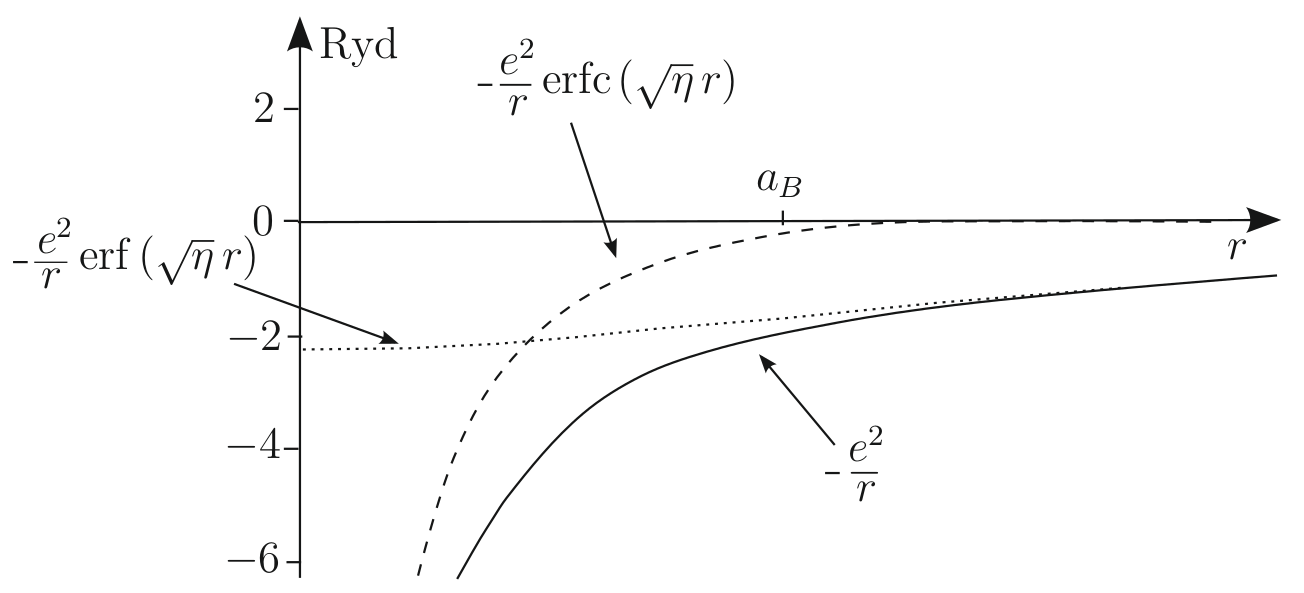
\includegraphics[height=1.2in,width=2.82in,viewport=0 0 1100 455,clip]{Figures/Ewald_method.png}
\caption{\fontsize{5.5pt}{2.2pt}\selectfont{\textrm{Decomposition of the potential $-e^2/r$ (singular at the origin and of long-range nature) into a contribution $-(e^2/r)\mathrm{erf}(\sqrt{\eta}r)$(regular at the origin of long-range) and a contribution $-(e^2/r)\mathrm{erfc}(\sqrt{\eta}r)$ (singular at the origin and of short-range nature). Here $\sqrt{\eta}=1 (\mathrm{Bohr radius unit})$ is chosen.}}}%(与文献\cite{EPJB33-47_2003}图1对比)
\label{Error_Function}
\end{figure}
}

\frame
{
	\frametitle{离子间相互作用的\textrm{Ewald}求和}
\begin{figure}[h!]
\centering
\vspace*{-0.20in}
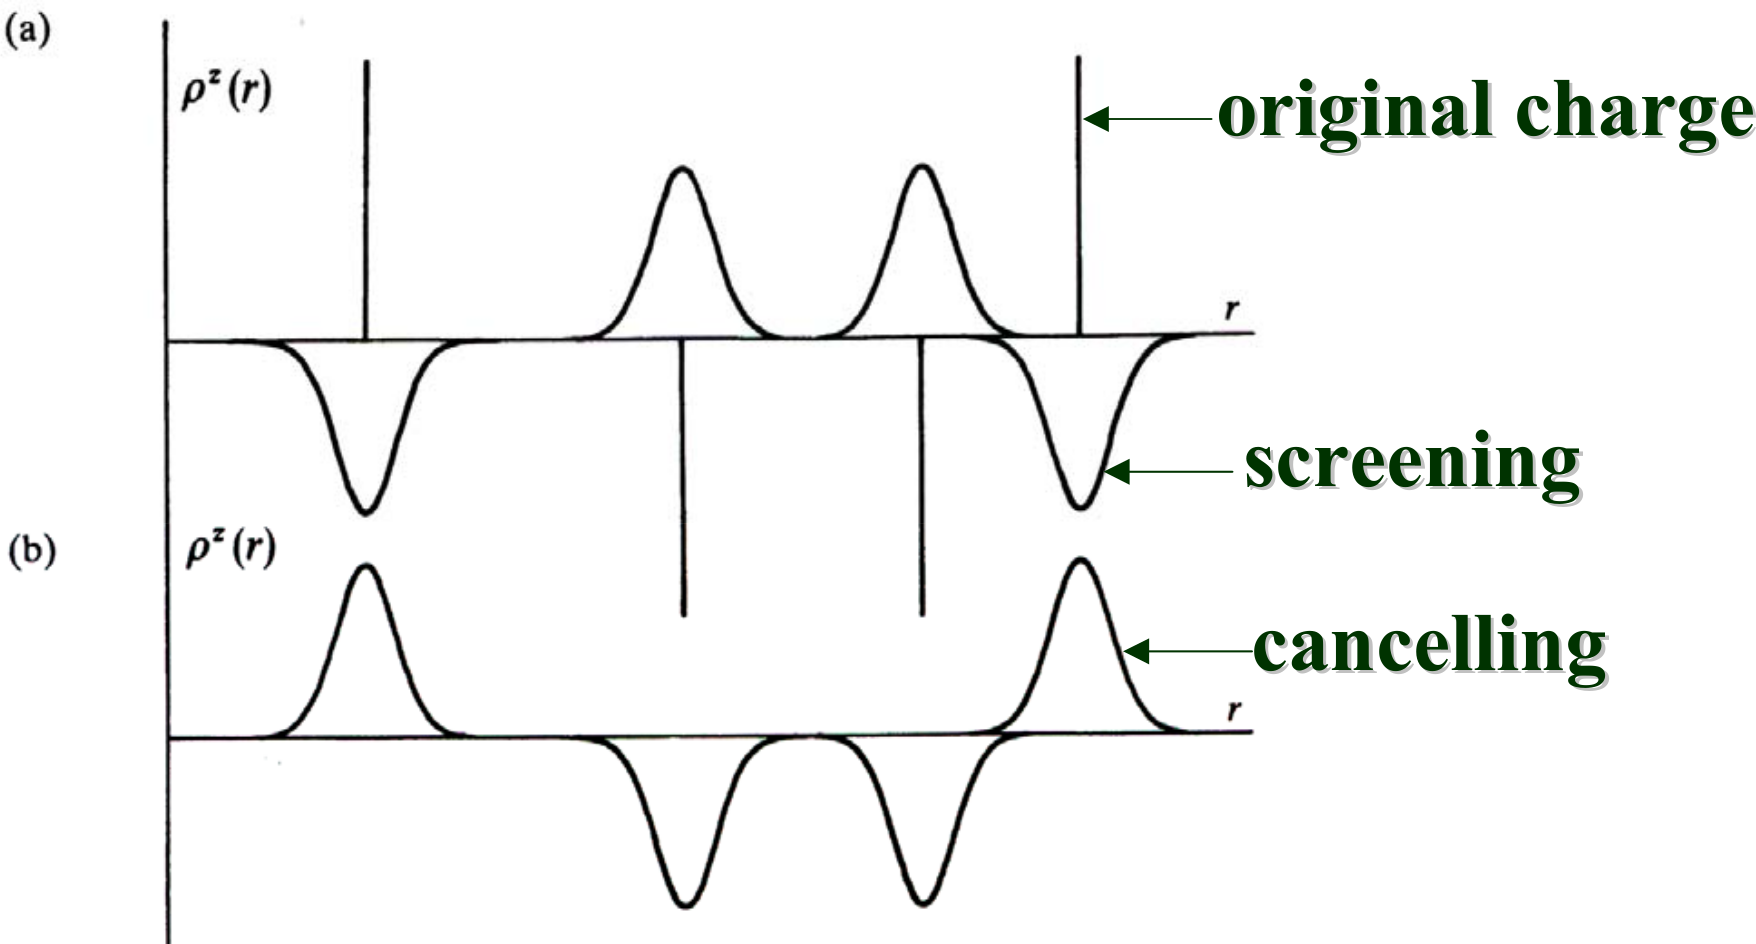
\includegraphics[height=1.6in,width=3.32in,viewport=0 0 1800 955,clip]{Figures/Ewald_method-2.png}
\caption{\fontsize{5.5pt}{2.2pt}\selectfont{\textrm{Each charge be screened by a Gaussian charge distribution of opposite sign and equal magnitude: $\rho_i(r)=\dfrac{Z_i\eta^3}{\pi^{3/2}}\mathrm{e}^{-\eta^2r^2}$.}}}%(与文献\cite{EPJB33-47_2003}图1对比)
\label{Ewald_method-2}
\end{figure}
\textrm{Particle mesh Ewald~(PME)}和\textrm{Particle-Particle Particle-Mesh~(PPPM)}算法:\\
空间离散化,应用快速\textrm{Fourier}变换\textrm{(Fast Fourier Transform, FFT)}将计算复杂度由$\mathscr{O}(N^2)$降为$\mathscr{O}(N\log(N))$
}

\frame
{
	\frametitle{邻居列表\textrm{(neighbour list)}}
	\begin{itemize}
		\item 遍历模拟体系全部任意两个粒子间距离的计算复杂度为$\mathscr{O}(N^2)$,实际计算中,对于短程相互作用,可以忽略远距离的长程作用,截断后的计算复杂度将大大下降
		\item \textcolor{blue}{\textrm{The minimum-image convention}}:\\为加速计算,将容器空间划分成小的立方体\textrm{(cell)},每个\textrm{cell}的边长为截断距离。计算粒子距离时,对于给定粒子只须遍历最近邻27个\textrm{cell}内的粒子(包括本身所在的\textrm{cell})。计算复杂度降为$\mathscr{O}(N)$
\begin{figure}[h!]
\centering
\vspace*{-0.18in}
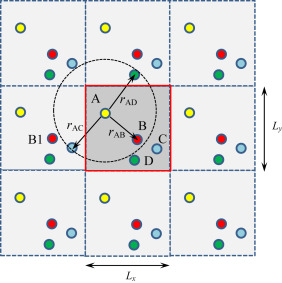
\includegraphics[height=1.2in,width=1.28in,viewport=0 0 180 180,clip]{Figures/Schematic-showing-the-closest-neighbors-of-atom_A-in-the-primary-simulation-cell-as-determined-by-the-minimum-image-criterion.jpg}
\caption{\fontsize{5.5pt}{2.2pt}\selectfont{\textrm{Schematic showing the closest neighbors of atom A in the primary simulation cell as determined by the minimum image criterion.}}}%(与文献\cite{EPJB33-47_2003}图1对比)
\label{Minimum-image-convention}
\end{figure}
	\end{itemize}
	
}

\subsection{数据分析}
\frame
{
	\frametitle{能量数据}
	\begin{itemize}
		\item 总能量~$E=E_{\mathrm{k}}+E_{\mathrm{p}}$
\begin{displaymath}
	\begin{aligned}
		E_{\mathrm{k}}=&\bigg\langle\sum\limits_{i=1}^N\dfrac12m_iv_i^2\bigg\rangle\\
		E_{\mathrm{p}}=&\bigg\langle\sum\limits_{i=1}^NE_{\mathrm{p}i}\bigg\rangle 
	\end{aligned}
\end{displaymath}
\item 比热容~$C_V^{\mathrm{NVT}}=\dfrac{\big\langle E_{\mathrm{p}}^2\big\rangle-\big\langle E_{\mathrm{p}}\big\rangle^2}{k_{\mathrm{B}}T^2}+\dfrac32Nk_{\mathrm{B}}$
\item 瞬时温度 ~$T=\dfrac2{\mathrm{d}Nk_{\mathrm{B}}}E_{\mathrm{k}}$ ~~~~ 其中$\mathrm{d}$是空间维度
\item 瞬时压强 ~$P=\rho k_{\mathrm{B}}T+\dfrac1{\mathrm{d}V}\bigg\langle\sum\limits_{i<j}\vec f_{ij}(\vec r_{ij})\cdot\vec r_{ij}\bigg\rangle$
	\end{itemize}
}

\frame
{
	\frametitle{相关系数}
	\begin{displaymath}
		\begin{aligned}
			c(A,B)&=\dfrac{\big\langle\big(A-\langle A\rangle\big)\big(B-\langle B\rangle\big)\big\rangle}{\sqrt{\big\langle\big(A-\langle A\rangle\big)^2\big\rangle\big\langle\big(B-\langle B\rangle\big)^2\big\rangle}}\\
			c&\in[0,1]
		\end{aligned}
	\end{displaymath}
	\begin{itemize}
		\item 时间相关系数\\
			\begin{displaymath}
				c(A,B,t)=\dfrac{\big\langle\big(A(t+t_0)-\langle A(t+t_0)\rangle\big)\big(B(t_0)-\langle B(t_0)\rangle\big)\big\rangle}{\sqrt{\big\langle\big(A(t+t_0)-\langle A(t+t_0)\rangle\big)^2\big\rangle\big\langle\big(B(t_0)-\langle B(t_0)\rangle\big)^2\big\rangle}}
			\end{displaymath}
		\item 时间自相关系数
			\begin{displaymath}
				c(A,t)=\dfrac{\big\langle\big(A(t+t_0)-\langle A(t+t_0)\rangle\big)\big(A(t_0)-\langle A(t_0)\rangle\big)\big\rangle}{\big\langle\big(A(t_0)-\langle A(t_0)\rangle\big)^2\big\rangle}
			\end{displaymath}
	\end{itemize}
}

\frame[allowframebreaks]
{
	\frametitle{结构特征}
	\begin{itemize}
		\item \textrm{Radial distribution function~(RDF)}:\\
			在距离$r$处找到粒子的概率
			\begin{displaymath}
				g(r)=\dfrac{V}{N^2}\bigg\langle\sum_i\sum_{j\neq i}\delta(\vec r-\vec r_{ij})\bigg\rangle
			\end{displaymath}
			理想气体~$g(r)=1$

\begin{figure}[h!]
\centering
\vspace*{-0.15in}
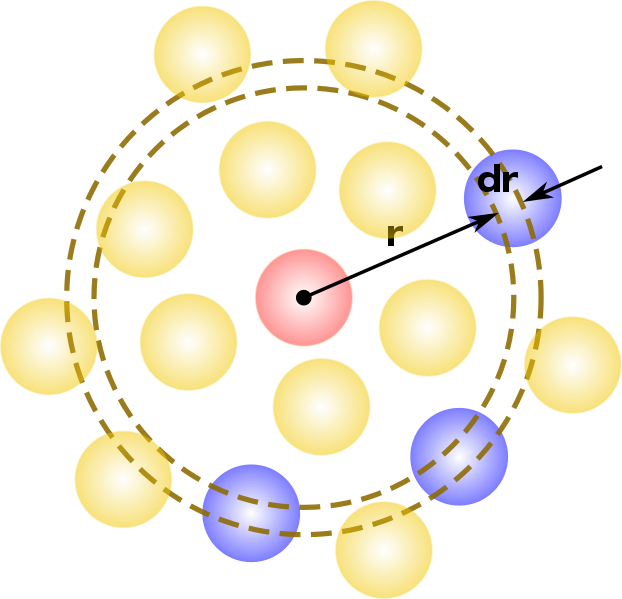
\includegraphics[height=1.0in,width=1.1in,viewport=0 0 630 600,clip]{Figures/Rdf_schematic.png}
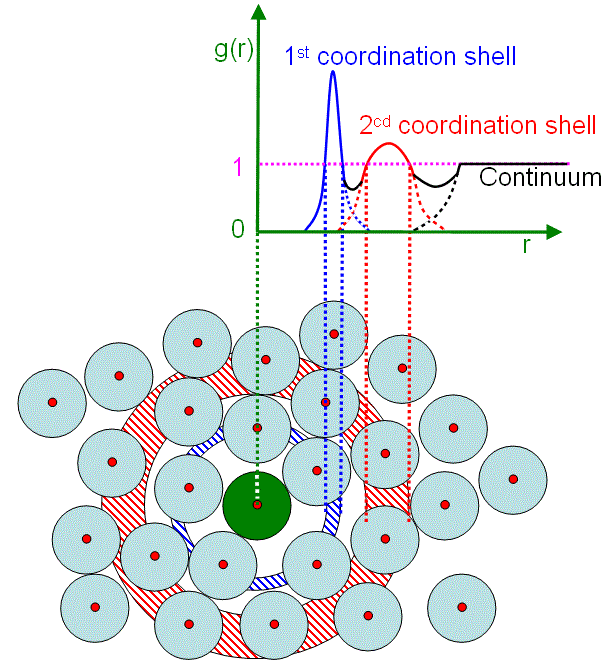
\includegraphics[height=1.0in,width=0.9in,viewport=0 0 610 660,clip]{Figures/Schematic-illustration-of-g(r)-dependence-on-r.png}
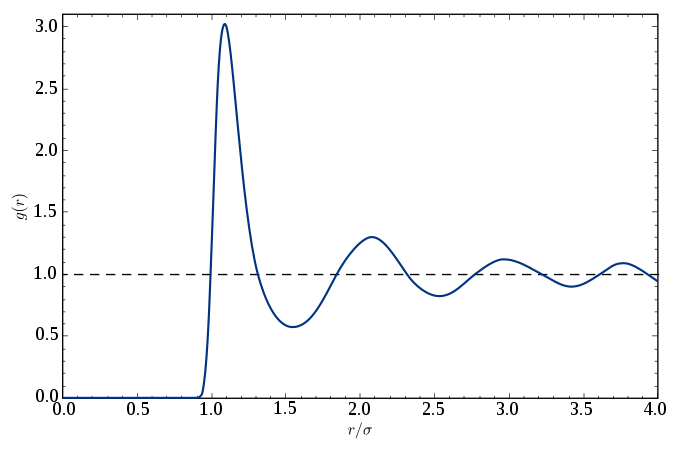
\includegraphics[height=1.0in,width=1.6in,viewport=0 0 680 480,clip]{Figures/Lennard-Jones_Radial_Distribution_Function.png}
\caption{\fontsize{5.5pt}{2.2pt}\selectfont{\textrm{Schematic illustration of g(r) dependence on r and the radial distribution function for Lennard-Jones fluid at $T^{\ast}=0.71$, $n^{\ast}=0.844$.}}}%(与文献\cite{EPJB33-47_2003}图1对比)
\label{Radial_distribution-function}
\end{figure}
		\item \textrm{Structure factor}:\\
			\textrm{RDF}在$\vec k$空间的\textrm{Fourier}变换,实验可直接观测的物理量
			\begin{displaymath}
				S(k)=1+4\pi\rho\int_0^{\infty}r^2\dfrac{\sin(\vec k\cdot\vec r)}{\vec k\cdot\vec r}g(r)\mathrm{d}r
			\end{displaymath}
\begin{figure}[h!]
\centering
\vspace*{-0.25in}
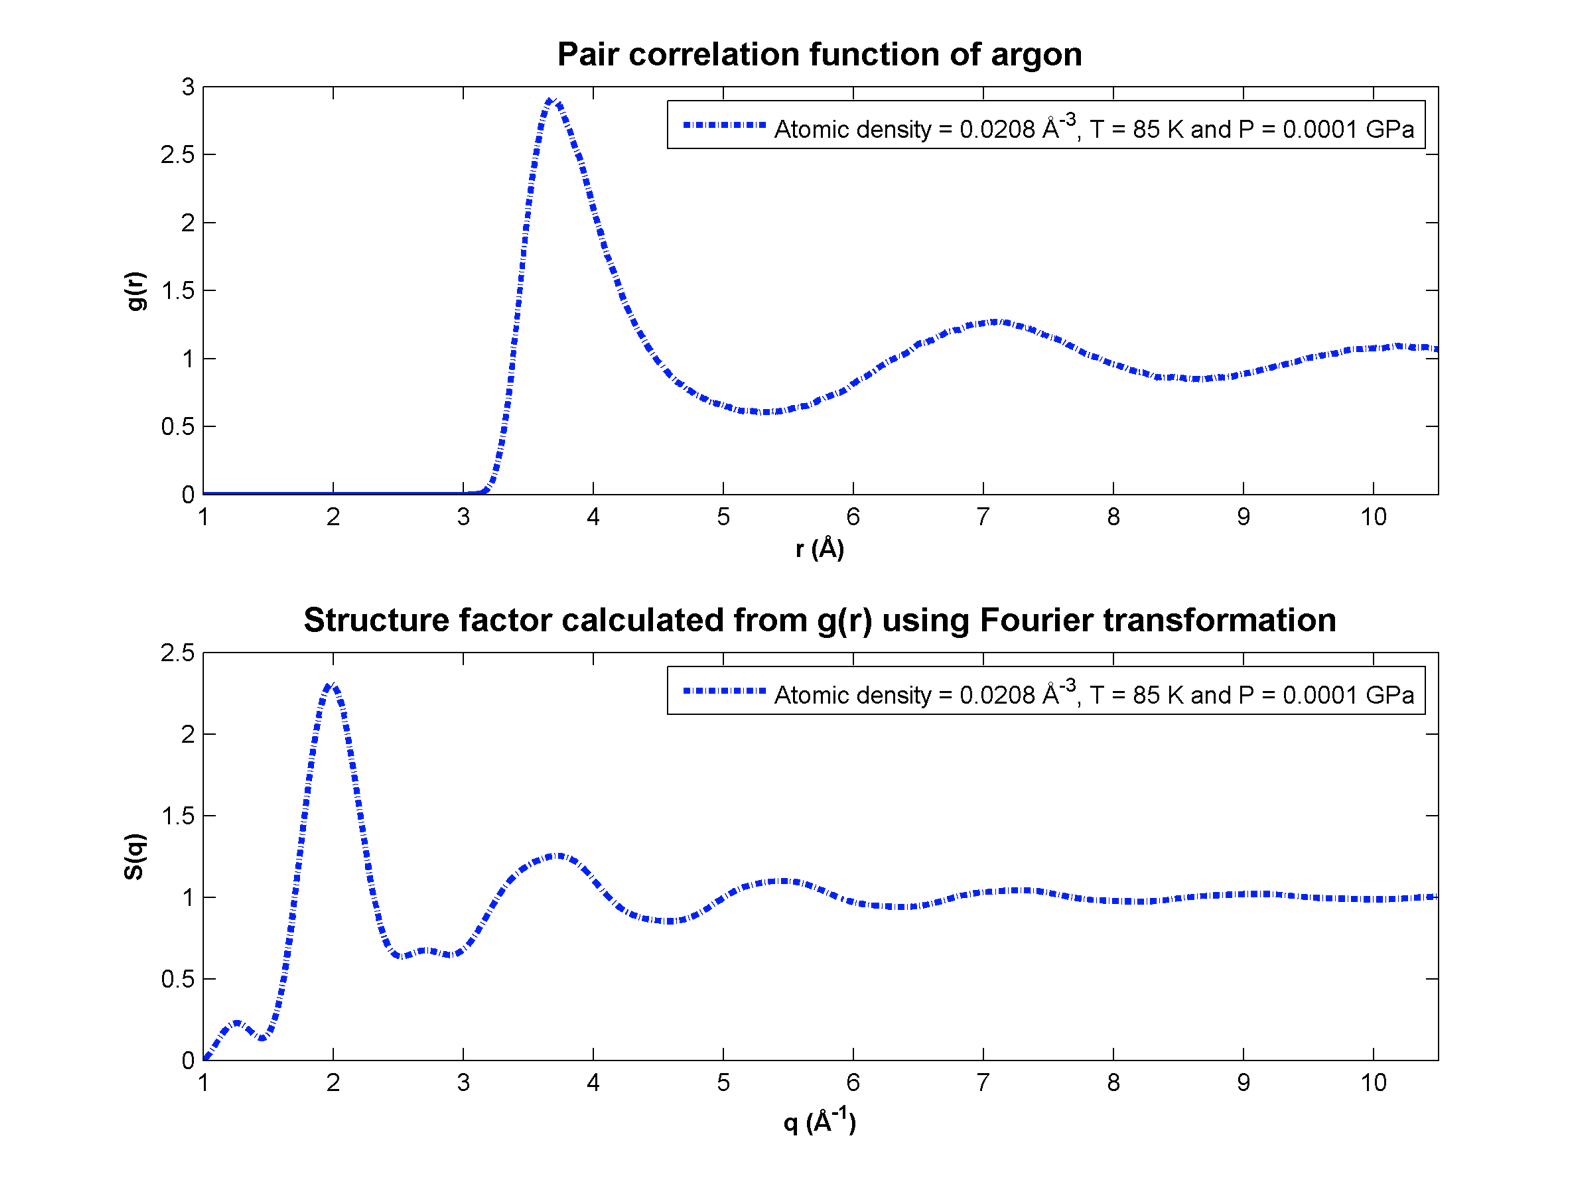
\includegraphics[height=1.4in,width=1.9in,viewport=60 10 730 580,clip]{Figures/Structure-factor-RDF.png}
\caption{\fontsize{5.5pt}{2.2pt}\selectfont{\textrm{The structure factor of argon calculating from a radial distribution function.}}}%(与文献\cite{EPJB33-47_2003}图1对比)
\label{Structure-factor}
\end{figure}
	\end{itemize}
}

\frame
{
	\frametitle{扩散系数}
	\begin{itemize}
		\item \textrm{Mean square displacement~(MSD)}:\\
			时间$t$间隔内粒子运动的平均距离的平方
			\begin{displaymath}
				\big\langle r^2(t)\big\rangle\equiv\big\langle\Delta r^2(t)\big\rangle=\dfrac1N\sum_{i=1}^N\Delta r_i^2(t)
			\end{displaymath}
		\item \textrm{Diffusion coefficient}:\\
			\begin{displaymath}
				\big\langle r^2(t)\big\rangle=2\mathrm{d}D\qquad\qquad \mbox{\textrm{d}是空间维度}
			\end{displaymath}
			\item \textrm{Velocity autocorelation function~(VACF)}:\\
				\begin{displaymath}
					\begin{aligned}
						&\big\langle\vec v(t)\vec v(0)\big\rangle\\
						D=&\int_0^{\infty}\langle\vec v(t)\vec v(0)\mathrm{d}t
					\end{aligned}
				\end{displaymath}

	\end{itemize}
}

\frame
{
	\frametitle{扩散系数}
\begin{figure}[h!]
\centering
\vspace*{-0.2in}
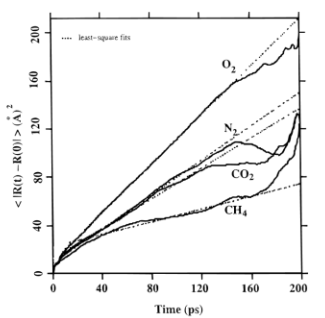
\includegraphics[height=1.2in,width=2.0in,viewport=0 0 350 300,clip]{Figures/MSD_O2-N2-CO2-CH4.png}\\
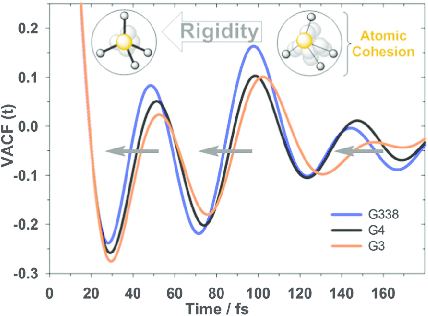
\includegraphics[height=1.6in,width=2.8in,viewport=0 0 230 160,clip]{Figures/The-velocity-autocorrelation-function-VACF-of-the-Al-atoms-showing-the-increase-of-rigidity of the local Al-coordination-for-G3-G4-and-G338-glasses.png}
%\caption{\fontsize{5.5pt}{2.2pt}\selectfont{\textrm{The structure factor of argon calculating from a radial distribution function.}}}%(与文献\cite{EPJB33-47_2003}图1对比)
\label{MSD-VACF}
\end{figure}
}

%\section{\rm{LAMMPS}常用命令}
%\frame
%{
%	\frametitle{\textcolor{cyan}{\textit{units}}:~定义单位类型}
%	\begin{itemize}
%		\item 语法:~\textcolor{cyan}{\textit{units}} \textrm{\textcolor{blue}{style}}
%		\item \textcolor{cyan}{\textit{units}}~命令用来定义模拟过程中使用的单位类型\\
%			{\fontsize{7.5pt}{5.2pt}\selectfont{决定了所有输入脚本、数据文件和所有输出到屏幕、日志文件以及\textrm{dump}文件中物理量的单位}}
%	\end{itemize}
%\textrm{\textcolor{blue}{style}}可取为
%\vskip 2pt
%\textrm{\textcolor{magenta}{lj} or \textcolor{magenta}{real} or \textcolor{magenta}{metal} or \textcolor{magenta}{si} or \textcolor{magenta}{cgs} or \textcolor{magenta}{electron} or \textcolor{magenta}{micro} or \textcolor{magenta}{nano}}
%\vskip 2pt
%{\fontsize{7.5pt}{5.2pt}\selectfont{金属中一般用\textrm{metal}}}
%}
%
%\frame
%{
%	\frametitle{\textcolor{cyan}{\textit{boundary}}:~设置模拟\textrm{box}的边界条件}
%	\begin{itemize}
%		\item 语法:~\textcolor{cyan}{\textit{boundary}} \textrm{$x$~$y$~$z$}
%		\item \textcolor{cyan}{\textit{boundary}}命令设置\textrm{box}的边界条件,参数\textrm{$x$~$y$~$z$}分别设置该维度的边界条件
%			\vskip 3pt
%			最基本的边界条件有四种:~\textrm{\textcolor{blue}{p}~\textcolor{blue}{f}~\textcolor{blue}{s}~\textcolor{blue}{m}}
%	\begin{itemize}
%			\setlength{\itemsep}{5pt}
%{\fontsize{7.5pt}{5.2pt}\selectfont{
%		\item \textrm{\textcolor{blue}{p}}是周期性边界:~当粒子从一侧飞出,会从相对应的另一侧再次进入\textrm{box},一般情况下不会发生\textrm{``lost~atoms''}(丢失原子)错误
%		\item \textrm{\textcolor{blue}{f}}是固定边界:~表示\textrm{box}的表面在该方向上被固定住,不因体系压力的变化发生移动,如果原子从一个表面飞出,会提示\textrm{``lost~atoms''}错误
%			\vskip 3pt
%			{\fontsize{6.2pt}{4.5pt}\selectfont{设置\textcolor{cyan}{\textit{thermo\_modify}}~\textrm{\textcolor{blue}{lost}}可以允许原子丢失,否则模拟过程会被终止}}
%		\item \textrm{\textcolor{blue}{s}}是收缩性边界条件:~表示在该方向上,盒子的表面会根据体系的压力大小或原子运动情况发生移动
%			\vskip 3pt
%			{\fontsize{6.2pt}{4.5pt}\selectfont{一般情况下,盒子会配合原子的移动,尽量把原子包含在\textrm{box}内,但是当原子速度过快,位移太大时原子也可能会飞出盒子,造成\textrm{``lost~atoms''}错误}}}}
%	\end{itemize}
%	\end{itemize}
%{\fontsize{7.0pt}{5.2pt}\selectfont{
%	\textrm{LAMMPS}\textcolor{blue}{支持对同一方向的两个边界设置不同的边界条件}:~
%	\vskip 4pt
%	对$y$方向下表面设置\textrm{\textcolor{blue}{f}}边界、上表面设置\textrm{\textcolor{blue}{s}}边界,可以写为:\\
%	\textcolor{cyan}{\textit{boundary}}~ \textcolor{blue}{\textrm{p}}~\textcolor{blue}{\textrm{fs}}~\textcolor{blue}{\textrm{p}}}}
%}
%
%\frame
%{
%	\frametitle{\textcolor{cyan}{\textit{atom\_style}}:~定义模拟过程中原子的类型}
%	\begin{itemize}
%		\item 语法:~\textcolor{cyan}{\textit{atom\_style}} \textrm{\textcolor{blue}{style}}
%		\item \textcolor{cyan}{\textit{atom\_style}}命令用来定义模拟过程中原子的类型:~\\
%			{\fontsize{7.5pt}{5.2pt}\selectfont{\textcolor{red}{不同的对象粒子所具有的属性不同,对于某个粒子对象,粒子不存在的属性就不需要设置,以便节省内存,加速运算}}}
%	\end{itemize}
%			\textrm{\textcolor{blue}{style}}可取为\\
%			\textrm{\textcolor{magenta}{amoeba} or \textcolor{magenta}{angle} or \textcolor{magenta}{atomic} or \textcolor{magenta}{body} or \textcolor{magenta}{bond} or \textcolor{magenta}{charge} or \textcolor{magenta}{dipole} or \textcolor{magenta}{dpd} or \textcolor{magenta}{edpd} or \textcolor{magenta}{electron} or \textcolor{magenta}{ellipsoid} or \textcolor{magenta}{full} or \textcolor{magenta}{line} or \textcolor{magenta}{mdpd} or \textcolor{magenta}{molecular} or \textcolor{magenta}{oxdna} or \textcolor{magenta}{peri} or \textcolor{magenta}{smd} or \textcolor{magenta}{sph} or \textcolor{magenta}{sphere} or \textcolor{magenta}{bpm}/\textcolor{magenta}{sphere} or \textcolor{magenta}{spin} or \textcolor{magenta}{tdpd} or \textcolor{magenta}{tri} or \textcolor{magenta}{template} or \textcolor{magenta}{hybrid}}
%\vskip 3pt
%{\fontsize{6.2pt}{5.2pt}\selectfont{
%	当\textrm{\textcolor{blue}{style}}为\textcolor{magenta}{\textrm{full}}时,其属性包括:~粒子编号,粒子所属分子的编号,粒子类别\textrm{(atom type)},带电电荷量,坐标$x$,$y$,$z$\\
%如果粒子是金属粒子,如\textrm{Fe},粒子\textrm{style}为\textcolor{magenta}{\textrm{atomic}}的属性是:~粒子编号,粒子类别,坐标$x$,$y$,$z$}}
%}
%
%\frame
%{
%	\frametitle{\textcolor{cyan}{\textit{variable}}:~定义一个变量}
%	\begin{itemize}
%		\item 语法:~\textcolor{cyan}{\textit{variable}} \textrm{\textcolor{blue}{name style $\cdots$}}\\
%			{\fontsize{7.5pt}{5.2pt}\selectfont{\textcolor{blue}{\textrm{name}}是用户定义的变量名}}
%		\item \textcolor{cyan}{\textit{variable}}是\textrm{LAMMPS}中定义变量的主要命令\\
%			{\fontsize{7.5pt}{5.2pt}\selectfont{在编写\textcolor{purple}{Input}文件时,用于循环程序,条件执行,控制体系运动,变化模拟参数,以及分布计算核心,提高计算效率方面非常有用}}
%	\end{itemize}
%			\textrm{\textcolor{blue}{style}}是变量类型,可取为\\
%			\textrm{\textcolor{magenta}{delete} or \textcolor{magenta}{index} or \textcolor{magenta}{loop} or \textcolor{magenta}{world} or \textcolor{magenta}{universe} or \textcolor{magenta}{uloop} or \textcolor{magenta}{string} or \textcolor{magenta}{format} or \textcolor{magenta}{getenv} or \textcolor{magenta}{file} or \textcolor{magenta}{atomfile} or \textcolor{magenta}{python} or \textcolor{magenta}{timer} or \textcolor{magenta}{internal} or \textcolor{magenta}{equal} or \textcolor{magenta}{vector} or \textcolor{magenta}{atom}}
%			\vskip 3pt
%{\fontsize{7.5pt}{5.2pt}\selectfont{常用的变量类型:}}
%	\begin{itemize}
%{\fontsize{7.5pt}{5.2pt}\selectfont{
%		\item \textrm{\textcolor{magenta}{index}}:~常搭配\textcolor{cyan}{\textit{next}}命令使用%,最开始将第一个字符串12赋予变量x,即x=12;后面遇到next命令时,在依次将后面的值赋予x
%			\\{\fontsize{6.2pt}{5.2pt}\selectfont{\textrm{E.g.:}~\textcolor{cyan}{\textit{variable}} \textrm{x} \textrm{\textcolor{magenta}{index}} \textrm{12 14 19 15 17}}}
%\item \textrm{\textcolor{magenta}{loop}}:~与\textrm{\textcolor{magenta}{index}}的作用相同,不同的是\textrm{\textcolor{magenta}{index}}后跟的字符串需要一一列出,而\textrm{\textcolor{magenta}{loop}}后面只需要写一个$n$即可\\
%	{\fontsize{6.2pt}{5.2pt}\selectfont{比如\textcolor{cyan}{\textit{variable}} \textrm{x} \textrm{\textcolor{magenta}{loop}} \textrm{140}代表了从\textrm{1}到\textrm{140}的列表,不需要像\textrm{\textcolor{magenta}{index}}一样一一列出}}}}
%	\end{itemize}
%}
%
%\frame[allowframebreaks]
%{
%	\frametitle{\textcolor{cyan}{\textit{lattice}}:~定义供其它命令使用的晶格}
%	\begin{itemize}
%		\item 语法:~\textcolor{cyan}{\textit{lattice}} \textrm{\textcolor{blue}{style scale keyword $\cdots$}} 
%		\item \textcolor{cyan}{\textit{lattice}}命令定义各式各样的晶格\\
%			{\fontsize{8.5pt}{5.2pt}\selectfont{\textcolor{cyan}{\textit{lattice}}在\textrm{LAMMPS}中的两种应用方式:}}
%	\begin{enumerate}
%{\fontsize{7.5pt}{5.2pt}\selectfont{
%		\item 利用\textcolor{cyan}{\textit{create\_atoms}}命令在模拟单元的晶格格点上创建原子\\
%			{\fontsize{6.2pt}{5.2pt}\selectfont{\textcolor{cyan}{\textit{create\_atom}}命令是给晶格格点原子位置上分配不同的原子类型}}
%		\item 被\textcolor{cyan}{\textit{create\_box}}, \textcolor{cyan}{\textit{region}}, \textcolor{cyan}{\textit{velocity}}等命令用作距离单位}}
%	\end{enumerate}
%\item \textrm{LAMMPS}中,晶格仅仅是空间中点的集合\\
%	模拟对象由最小重复单元(初基原胞)决定
%	\vskip 5pt
%	{\fontsize{8.0pt}{5.2pt}\selectfont{最小重复单元在所有维度中无限被复制}}
%	\end{itemize}
%%			\begin{itemize}
%			%	\item 
%	\textrm{\textcolor{blue}{style}}可取为\\
%					\textrm{\textcolor{magenta}{none} or \textcolor{magenta}{sc} or \textcolor{magenta}{bcc} or \textcolor{magenta}{fcc} or \textcolor{magenta}{hcp} or \textcolor{magenta}{diamond} or \textcolor{magenta}{sq} or \textcolor{magenta}{sq2} or \textcolor{magenta}{hex} or \textcolor{magenta}{custom}}
%\vskip 7pt			%	\item 
%					\textrm{\textcolor{blue}{scale}} \footnote{\fontsize{6.2pt}{5.2pt}\selectfont{\textrm{\textcolor{blue}{scale}}表示的标度关系:~\textrm{scale factor between lattice and simulation box}}}:~对于除了\textrm{L-J~units}外的所有其他单位,\textrm{scale}是以距离为单位的晶格常数\textrm{(lattice constant in distance units)}
%\vskip 7pt			%	\item 
%					\textrm{\textcolor{blue}{keyword}}可取为\\
%					\textrm{\textcolor{magenta}{origin} or \textcolor{magenta}{orient} or \textcolor{magenta}{spacing} or \textcolor{magenta}{$a_1$} or \textcolor{magenta}{$a_2$} or \textcolor{magenta}{$a_3$} or \textcolor{magenta}{bias}}
%\vskip 7pt			%	\item 
%	{\fontsize{8.5pt}{5.2pt}\selectfont{\textcolor{cyan}{\textit{lattice}}命令需要与模拟维度保持一致:
%	\begin{itemize}
%		\item \textrm{\textcolor{blue}{style}} \textrm{\textcolor{magenta}{sc} or \textcolor{magenta}{bcc} or \textcolor{magenta}{fcc} or \textcolor{magenta}{hcp} or \textcolor{magenta}{diamond}}被用于\textrm{3D}问题
%		\item \textrm{\textcolor{blue}{style}} \textrm{\textcolor{magenta}{sq} or \textcolor{magenta}{sq2} or \textcolor{magenta}{hex}} 被用于\textrm{2D}问题
%	\end{itemize}}}
%	{\fontsize{6.5pt}{5.2pt}\selectfont{\textcolor{red}{\textrm{E.g:}}
%	\vskip 3pt
%	\textcolor{cyan}{\textit{lattice}} \textrm{fcc 4.05}
%	\vskip 3pt
%	表示晶格类型是\textrm{fcc},晶格常数为\textrm{4.05},单位是\textrm{\AA}}}
%}
%
%\frame
%{
%	\frametitle{\textcolor{cyan}{\textit{region}}:~定义空间几何区域}
%	\begin{itemize}
%		\item 语法:~\textcolor{cyan}{\textit{region}} \textrm{\textcolor{blue}{ID style keyword $\cdots$}}
%	\end{itemize}
%%			\begin{itemize}
%%				\item 
%					\textrm{\textcolor{blue}{ID}}:~用户为区域命的名
%\vskip 7pt			%	\item 
%					\textrm{\textcolor{blue}{style}}可取为\textrm{\textcolor{magenta}{delete} or \textcolor{magenta}{block} or \textcolor{magenta}{cone} or \textcolor{magenta}{cylinder} or \textcolor{magenta}{ellipsoid} or \textcolor{magenta}{plane} or \textcolor{magenta}{prism} or \textcolor{magenta}{sphere} or \textcolor{magenta}{union} or \textcolor{magenta}{intersect}}
%					\begin{itemize}
%{\fontsize{7.5pt}{5.2pt}\selectfont{
%\item \textrm{\textcolor{magenta}{delete}}:~没有参数
%\item \textrm{\textcolor{magenta}{block}}:~\textrm{xlo xhi ylo yhi zlo zhi}是三个维度上的最小值和最大值
%\item \textrm{\textcolor{magenta}{cone}}:~\textrm{dim c1 c2 radlo radhi lo hi}}}
%					\end{itemize}
%%			\end{itemize}
%{\fontsize{7.5pt}{5.2pt}\selectfont{
%	\textcolor{red}{举例如下}
%	\vskip 5pt
%	\textcolor{cyan}{\textit{lattice}} \textrm{fcc 4.05}\\
%	\textcolor{cyan}{\textit{region}} \textrm{box1 \textcolor{magenta}{block} 0 30 0 30 0 30}}}
%	\vskip 5pt
%{\fontsize{6.2pt}{5.2pt}\selectfont{
%	创建一个名字为\textrm{box1}的\textrm{\textcolor{magenta}{block}},其中$x$, $y$, $z$方向上的长度均为30倍的晶格常数\\
%	\textcolor{red}{注意}:~这里的\textrm{30}是\textrm{30}倍的意思,实际长度为\textrm{30}乘以\textrm{4.05~\AA}
%	\vskip 4pt
%	如果想要让\textrm{30}代表实际长度,即让其单位为\AA,则只需要在后面加上\textcolor{cyan}{\textit{units}} \textrm{box}即可:\\
%	\textcolor{cyan}{\textit{region}} \textrm{box1 \textcolor{magenta}{block} 0 30 0 30 0 30} \textcolor{cyan}{\textit{units}} \textrm{box}}}
%}
%
%\frame
%{
%	\frametitle{\textcolor{cyan}{\textit{create\_box}}:~创建一个有限区域}
%	\begin{itemize}
%	\item 语法:~\textcolor{cyan}{\textit{create\_box}} \textrm{N region-ID \textcolor{blue}{keyword} $\cdots$}
%	\item 该命令还固定了该模拟区域中原子类型
%	\end{itemize}
%		\textrm{N}:~本次模拟使用的原子种类数
%\vskip 7pt			%	\item 
%		\textrm{region-ID}:~用来模拟的区域的\textrm{ID}
%\vskip 7pt			%	\item 
%		\textrm{\textcolor{blue}{keyword}}可取为\\
%		\textrm{\textcolor{magenta}{bond}/\textcolor{magenta}{types} or \textcolor{magenta}{angle}/\textcolor{magenta}{types} or \textcolor{magenta}{dihedral}/\textcolor{magenta}{types} or \textcolor{magenta}{improper}/\textcolor{magenta}{types} or \textcolor{magenta}{extra}/\textcolor{magenta}{bond}/\textcolor{magenta}{per}/\textcolor{magenta}{atom} or \textcolor{magenta}{extra}/\textcolor{magenta}{angle}/\textcolor{magenta}{per}/\textcolor{magenta}{atom} or \textcolor{magenta}{extra}/\textcolor{magenta}{dihedral}/\textcolor{magenta}{per}/\textcolor{magenta}{atom} or \textcolor{magenta}{extra}/\textcolor{magenta}{improper}/\textcolor{magenta}{per}/\textcolor{magenta}{atom} or \textcolor{magenta}{extra}/\textcolor{magenta}{special}/\textcolor{magenta}{per}/\textcolor{magenta}{atom}}
%		\vskip 4pt
%{\fontsize{7.5pt}{5.2pt}\selectfont{
%	\textcolor{red}{举例如下}
%	\vskip 4pt
%	\textcolor{cyan}{\#}~在模拟盒子\textrm{box1}中添加一类原子\\
%	\textcolor{cyan}{\textit{create\_box}} \textrm{1 box1}}}
%}
%
%\frame
%{
%	\frametitle{\textcolor{cyan}{\textit{create\_atoms}}和\textcolor{cyan}{\textit{mass}}}
%	\begin{itemize}
%		\item \textcolor{cyan}{\textit{create\_atoms}}:~在指定区域内填充一定数量的原子\\
%	语法:~\textcolor{cyan}{\textit{create\_atoms}} \textrm{\textcolor{blue}{type style keyword $\cdots$}}
%	\vskip 4pt
%	{\fontsize{7.5pt}{5.2pt}\selectfont{其中\textrm{\textcolor{blue}{type}}与后面定义的模拟原子中的信息(\textcolor{cyan}{\textit{mass}})对应
%	\vskip 4pt
%	\textcolor{red}{举例如下}
%	\vskip 4pt
%	\textcolor{cyan}{\#} 在整个模拟区域中添加类型为\textrm{1}的原子(即添加\textrm{Al}原子)\\
%	\textcolor{cyan}{\textit{create\_atoms}} \textrm{1} \textcolor{cyan}{\textit{region}} \textrm{\textcolor{magenta}{whole}}
%	\vskip 4pt
%	\textcolor{cyan}{\#} 模拟环境中的原子信息\\
%	\textcolor{cyan}{\textit{mass}} \textrm{1 26.981   \textcolor{cyan}{\#} Al}\\
%	\textcolor{cyan}{\textit{mass}} \textrm{2 55.845   \textcolor{cyan}{\#} Fe}}}
%
%\item \textcolor{cyan}{\textit{mass}}:~为某一种或几种类型的原子设置质量
%	\end{itemize}
%}
%
%\frame
%{
%	\frametitle{\textcolor{cyan}{\textit{pair\_style}}和\textcolor{cyan}{\textit{pair\_coeff}}}
%	设置势函数\\
%	{\fontsize{7.5pt}{5.2pt}\selectfont{金属中常用的势函数是\textrm{EAM}势函数}}
%
%	\textrm{\textcolor{magenta}{$\ast$ $\ast$}}~是通配符:~意思是\textcolor{purple}{使原子之间存在相互作用}\footnote{\fontsize{6.2pt}{5.2pt}\selectfont{假如体系中有两类原子,\textrm{Al}和\textrm{Fe}原子,这个通配符的作用就是使\textrm{Al}原子与\textrm{Al}原子相互作用,\textrm{Fe}原子与\textrm{Fe}原子相互作用,\textrm{Al}原子和\textrm{Fe}原子相互作用}}
%	\vskip 4pt
%{\fontsize{7.5pt}{5.2pt}\selectfont{
%	\textcolor{red}{举例如下}
%	\vskip 4pt
%	\textcolor{cyan}{\textit{pair\_style}} \textrm{eam/alloy}\\
%	\textcolor{cyan}{\textit{pair\_coeff}}	\textcolor{magenta}{$\ast$} \textcolor{magenta}{$*$} \textrm{Al99.eam.alloy Al}}}\\
%	{\fontsize{6.2pt}{5.2pt}\selectfont{其中\textrm{Al99.eam.alloy}是势函数的名称}}
%	\vskip 8pt
%	\textcolor{red}{不同势函数后面的\textcolor{cyan}{\textit{pair\_coeff}}写法不同}\\
%{\fontsize{7.5pt}{5.2pt}\selectfont{
%	\textrm{EAM}势函数需要在后面写出所有原子的名称,且写的顺序要和\textcolor{cyan}{\textit{mass}}中定义的顺序一一对应}}
%}
%
%\frame[allowframebreaks]
%{
%	\frametitle{\textcolor{cyan}{\textit{group}}:~对原子分组}
%	\begin{itemize}
%		\item 分组后的原子会有一个\textrm{group-ID},\textrm{group-ID}将被用到\textcolor{cyan}{\textit{fix}}, \textcolor{cyan}{\textit{compute}}, \textcolor{cyan}{\textit{dump}}等命令中\\
%{\fontsize{7.5pt}{5.2pt}\selectfont{
%	如\textcolor{cyan}{\textit{fix}}命令中的第二个参数就是\textrm{group-ID}\\
%	\textcolor{cyan}{\textit{fix}} \textrm{ID group-ID style\_name \textcolor{blue}{keyword} $\cdots$}\\
%	\textcolor{cyan}{\textit{fix}} \textrm{1 water \textcolor{magenta}{npt} \textcolor{blue}{temp} 300.0 300.0 100.0 \textcolor{blue}{iso} 0.0 0.0 1000.0}}}
%\item 即使不对原子进行分组,\textrm{LAMMPS}也会设置一个默认的原子组:~\textrm{\textcolor{blue}{all}},也就是把所有的原子全部划分到\textrm{\textcolor{blue}{all}}组内\\
%{\fontsize{7.5pt}{5.2pt}\selectfont{
%	例如对系统所有原子进行温度初始化,可以使用下面的语句,其中\textrm{\textcolor{blue}{all}}就是默认的\textrm{group-ID}:~\\
%	\textcolor{cyan}{\textit{velocity}} \textrm{\textcolor{blue}{all} \textcolor{magenta}{create} 300.0 300.0 4928459}}}
%	\end{itemize}
%常用的分组方式有以下几种:
%\begin{enumerate}
%	\item 配合\textcolor{cyan}{\textit{region}}使用,把某一区域的原子归入到一个组中\\
%{\fontsize{7.5pt}{5.2pt}\selectfont{
%例如在纳米铜的拉伸时,需要一端固定,另一端施加一定的速度进行拉伸,这就需要把\textrm{Cu}原子划分为三个组:
%\begin{figure}[h!]
%\centering
%\vskip -10pt
%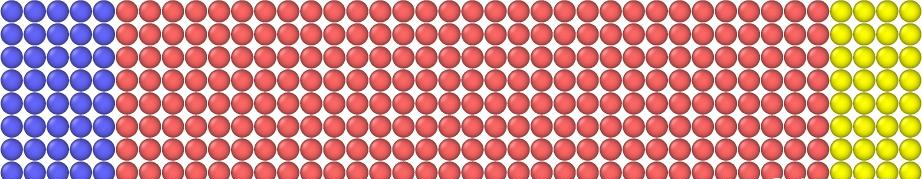
\includegraphics[height=0.70in,width=4.0in, viewport=0 0 270 50,clip]{Figures/Lammps_tutorial-command_group.png}
%%\caption{\fontsize{6.2pt}{5.2pt}\selectfont{\textrm{The general workflow for running molecular dynamics simulations using LAMMPS.}}}%(与文献\cite{EPJB33-47_2003}图1对比)
%\label{Lammps_tutorial-command_group}
%\end{figure}
%\begin{itemize}
%{\fontsize{7.5pt}{5.2pt}\selectfont{
%	\item \textrm{left}:~固定组
%	\item \textrm{right}:~速度加载组
%	\item \textrm{mobile}:~中间组}}
%\end{itemize}
%\textcolor{cyan}{\textit{group}}命令配合 \textcolor{magenta}{\textrm{union}}关键字可实现两个组的合并:\\
%{\fontsize{6.2pt}{5.2pt}\selectfont{
%例如\textrm{left}和\textrm{right}组合并为\textrm{boundary}组,可以写成:\\
%\textcolor{cyan}{\textit{group}} \textrm{boundary \textcolor{magenta}{union} left right}}}
%\vskip 3pt
%\textcolor{cyan}{\textit{group}}命令配合\textcolor{magenta}{\textrm{subtract}}关键字可实现减法操作:\\
%{\fontsize{6.2pt}{5.2pt}\selectfont{所有原子减去\textrm{boundary}原子即为中间\textrm{moible}原子,可以写为:\\
%\textcolor{cyan}{\textit{group}} \textrm{mobile \textcolor{magenta}{subtract} \textcolor{blue}{all} boundary}}}
%\vskip 5pt
%		\textrm{Cu}拉伸建模全部代码如下:
%		\verbatiminput{Figures/Lammps_tutorial-command_example.txt}}} %为保险:~选用文件名绝对路径
%\item 配合\textcolor{cyan}{\textit{type}}命令,可以将多种类型的原子归为一组
%	\vskip 3pt
%{\fontsize{7.5pt}{5.2pt}\selectfont{
%	\textcolor{cyan}{\#} 将原子类型为\textrm{3}和\textrm{4}的原子全部归入到\textrm{water}组\\
%	\textcolor{cyan}{\textit{group}} \textrm{water type 3 4}}}
%
%\item 配合原子\textrm{id}可将特定的原子归入到一组
%	{\fontsize{7.5pt}{6.0pt}\selectfont{
%		\verbatiminput{Figures/Lammps_tutorial-command_group.txt}}} %为保险:~选用文件名绝对路径
%\end{enumerate}
%\textcolor{red}{注意}:~\textrm{LAMMPS}最多支持\textrm{32}个\textcolor{cyan}{\textit{group}}(包含\textrm{\textcolor{blue}{all}}组)
%\vskip 4pt
%{\fontsize{7.5pt}{6.0pt}\selectfont{
%如果定义的组过多,可将不再使用的组删除:\\
%\textcolor{cyan}{\textit{group}} \textrm{boundary \textcolor{magenta}{delete}}}}
%}
%
%\frame[allowframebreaks]
%{
%	\frametitle{\textcolor{cyan}{\textit{set}}:~改变原子类型}
%	\begin{itemize}
%		\item 改变原子类型,可用来为不同区域设置不同颜色\\
%			{\fontsize{7.5pt}{6.0pt}\selectfont{特别是在高熵合金建模过程中}}
%	\end{itemize}
%{\fontsize{7.5pt}{6.0pt}\selectfont{
%	以下实例是在高熵合金建模中,包含的命令
%	\vskip 4pt
%	\textcolor{cyan}{\textit{set}} \textrm{\textcolor{blue}{type} type\_ID \textcolor{magenta}{type}/\textcolor{magenta}{ratio} type\_new fraction seed}
%	\begin{itemize}
%		\item \textrm{type\_ID}是需要被替换的原子类型
%		\item \textrm{type\_nea}是将要转换的新原子类型
%		\item \textrm{fraction}是新原子类型占初始原子类型的比例
%		\item \textrm{seed}为随机种子
%	\end{itemize}
%		\verbatiminput{Figures/Lammps_tutorial-command_set.txt}}} %为保险:~选用文件名绝对路径
%}
%
%\frame
%{
%	\frametitle{\textcolor{cyan}{\textit{write\_data}}和\textcolor{cyan}{\textit{timestep}}}
%	\begin{itemize}
%		\item \textcolor{cyan}{\textit{write\_data}}:~保存\textrm{data}文件\\
%			在\textcolor{red}{\textrm{ovitio}}中可视化后可用于验证模型是否正确
%\vskip 4pt
%{\fontsize{7.5pt}{6.0pt}\selectfont{
%	\textcolor{red}{举例如下}\\
%	\textcolor{cyan}{\textit{write\_data}} \textrm{Al\_model.xyz}}}
%
%\item \textcolor{cyan}{\textit{timestep}}:~设置模拟的时间步长
%	\vskip 4pt
%{\fontsize{7.5pt}{6.0pt}\selectfont{
%	金属中一般是在\textcolor{magenta}{\textrm{atomic}}单位制下,所以\textcolor{cyan}{\textit{timestep}}的单位一般是\textrm{ps}
%\vskip 4pt
%	\textcolor{red}{举例如下}\\
%	\textcolor{cyan}{\textit{timestep}} \textrm{0.001}}}\\
%	{\fontsize{6.2pt}{6.0pt}\selectfont{这里设置的是\textrm{0.001ps},也就是\textrm{1fs}}}
%	\end{itemize}
%}
%
%\frame
%{
%	\frametitle{\textcolor{cyan}{\textit{velocity}}:~创建初始温度}
%	\begin{itemize}
%		\item \textcolor{cyan}{\textit{velocity}} \textrm{group-ID \textcolor{blue}{style} \textcolor{blue}{keyword} $\cdots$}
%		\item \textcolor{cyan}{\textit{velocity}}用来创建初始温度,或者理解为原子组创建初始速度\footnote{\fontsize{6.2pt}{6.0pt}\selectfont{\textrm{LAMMPS}中温度的变化就是对应了速度的变化}}
%	\end{itemize}
%%		\item 
%	\textrm{group-ID}:~即将改变速度的原子组的\textrm{ID}
%\vskip 7pt			%	\item 
%	\textrm{\textcolor{blue}{style}}可取为\\
%	\textrm{\textcolor{magenta}{create} or \textcolor{magenta}{set} or \textcolor{magenta}{scale} or \textcolor{magenta}{ramp} or \textcolor{magenta}{zero}}
%	\vskip 5pt
%{\fontsize{7.5pt}{6.0pt}\selectfont{
%			\textrm{\textcolor{magenta}{create}}后面要跟用户指定的初始温度\textrm{temp seed} \textrm{(其中temp = temperature value (temperature units))}
%\vskip 4pt
%	\textcolor{red}{举例如下}\\
%	\textcolor{cyan}{\textit{velocity}} \textrm{\textcolor{blue}{all} \textcolor{magenta}{create} 300 12345}}}
%	\vskip 3pt
%{\fontsize{6.2pt}{6.0pt}\selectfont{
%	\textrm{\textcolor{blue}{all}是\textrm{LAMMPS}的关键字,表示所有原子,也可以改成\textrm{group-ID}\\
%	\textrm{\textcolor{magenta}{create} 300}意思是创建初始温度为\textrm{300K}\\
%	后面的\textrm{12345}是随机种子}}}
%}
%
%\frame[allowframebreaks]
%{
%	\frametitle{\textcolor{cyan}{\textit{fix}}}
%	\begin{itemize}
%		\item 语法:~\textcolor{cyan}{\textit{fix}} \textrm{ID group-ID \textcolor{blue}{style} \textcolor{blue}{keyword} $\cdots$}
%	\end{itemize}
%	 \textrm{ID:~user-assigned name for the fix}
%\vskip 7pt			%	\item 
%		\textrm{group-ID: ID of the group of atoms to apply the fix to}
%\vskip 7pt			%	\item 
%		\textrm{\textcolor{blue}{style}:~ one of a long list of possible style names}\\
%			可取为\\
%			\textrm{\textcolor{magenta}{nvt} or \textcolor{magenta}{npt} or \textcolor{magenta}{nph}}
%\vskip 7pt			%	\item 
%		\textrm{args:~arguments used by a particular style}
%		\vskip 4pt
%{\fontsize{7.5pt}{6.0pt}\selectfont{
%	\textcolor{red}{举例如下}\\
%	\textcolor{cyan}{\textit{fix}} \textrm{1 \textcolor{blue}{all} \textcolor{magenta}{npt} \textcolor{blue}{temp} 300 300 0.1 \textcolor{blue}{iso} 0 0 1 drag 1}}}
%	\begin{itemize}
%{\fontsize{7.5pt}{6.0pt}\selectfont{
%\item \textrm{1}是该\textcolor{cyan}{\textit{fix}}命令的\textrm{ID}
%\item \textcolor{blue}{\textrm{all}}是对所有原子施加后面的条件
%\item \textcolor{magenta}{\textrm{npt}}是等温等压系综
%\item \textcolor{blue}{\textrm{temp}}是设置温度的关键字\\
%	\textcolor{blue}{\textrm{temp}} \textrm{300 300 0.1}命令中\\
%	第一个参数\textrm{300}是\textcolor{red}{初始温度}\\
%	第二个参数\textrm{300}是\textcolor{red}{截止温度}\\
%	第三个参数\textrm{0.1}是温度的阻尼系数,设置它是使其在升温或者降温过程中不会出现太大的波动\footnote{\fontsize{6.2pt}{6.0pt}\selectfont{一般来说阻尼系数是\textrm{100}倍的\textcolor{cyan}{\textit{timestep}}}}\\
%\item \textrm{\textcolor{blue}{iso}}是控压方式,因为设置的是\textrm{\textcolor{magenta}{npt}}系综,所以温度和压力必须设置\\
%	其中\textrm{\textcolor{blue}{iso}}是对$x$,$y$,$z$三个方向进行联合控压(耦合控压)\footnote{\fontsize{6.2pt}{6.0pt}\selectfont{在控压时要改变模拟盒子的大小,$x$,$y$,$z$三个方向同时改变}}\\
%	与之相对的是\textrm{\textcolor{blue}{aniso}},是非耦合控压($x$,$y$,$z$三个方向不是同时改变)
%	\vskip 4pt
%	\textrm{\textcolor{blue}{iso}}后跟的是初始压强,结束压强,和阻尼系数(为了使压强在增加或者降低过程中不会出现太大波动)}}
%	\end{itemize}
%}
%
%\frame[allowframebreaks]
%{
%	\frametitle{\textcolor{cyan}{\textit{thermo}}和\textcolor{cyan}{\textit{thermo\_style}}}
%	设置输出信息/格式
%	\begin{itemize}
%		\item \textcolor{cyan}{\textit{thermo}} \textcolor{blue}{$N$}\\
%			\textcolor{blue}{$N$}:~\textrm{output thermodynamics every \textcolor{blue}{$N$}} \textcolor{cyan}{\textit{timesteps}}
%		\item \textcolor{cyan}{\textit{thermo\_style}} \textrm{\textcolor{blue}{style}}\\
%			\textrm{\textcolor{blue}{style}}可取为\\
%			\textrm{\textcolor{magenta}{one} or \textcolor{magenta}{multi} or \textcolor{magenta}{yaml} or \textcolor{magenta}{custom}}\\
%			\textrm{args:~list of arguments for a particular style}
%	\end{itemize}
%	\vskip 4pt
%{\fontsize{7.5pt}{6.0pt}\selectfont{
%	\textcolor{red}{举例如下}
%	\vskip 4pt
%	\textcolor{cyan}{\textit{thermoa}} \textrm{1000}\\
%%	\vskip 3pt
%	\textcolor{cyan}{\textit{thermo\_style}} \textrm{\textcolor{magenta}{custom} \textcolor{blue}{step} lx ly lz \textcolor{blue}{press} pxx pyy pzz \textcolor{blue}{pe} \textcolor{blue}{temp}}}}\\
%{\fontsize{6.2pt}{6.0pt}\selectfont{
%	\textcolor{cyan}{\textit{thermoa}} \textrm{1000}:~每1000步在屏幕上输出一次
%	\vskip 3pt
%	\textcolor{cyan}{\textit{thermo\_style}}后面是在屏幕上输出的信息:~
%	\vskip 3pt
%	\textrm{\textcolor{magenta}{custom}}后的内容就是在屏幕上输出的,可以看到
%	\vskip 4pt
%	输出的运行步数\textrm{\textcolor{blue}{step}}:~三个方向上的长度\textrm{lx, ly, lz}
%	\vskip 3pt
%	模拟体系的压力\textrm{\textcolor{blue}{press}}:~三个方向上的压力\textrm{pxx, pyy, pzz}
%	\vskip 3pt
%	\textrm{\textcolor{blue}{pe}}是模拟体系的势能
%	\vskip 3pt
%	\textrm{\textcolor{blue}{temp}}是模拟体系的温度
%\begin{figure}[h!]
%\centering
%\vskip -5pt
%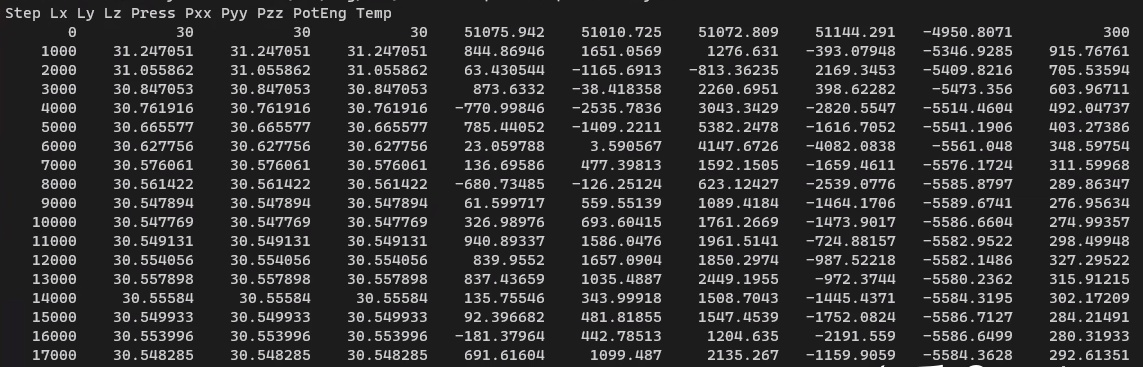
\includegraphics[height=1.40in,width=4.0in, viewport=0 1 280 90,clip]{Figures/Lammps_tutorial-command_thermo.png}
%%\caption{\fontsize{6.2pt}{5.2pt}\selectfont{\textrm{The general workflow for running molecular dynamics simulations using LAMMPS.}}}%(与文献\cite{EPJB33-47_2003}图1对比)
%\label{Lammps_tutorial-command_thermo}
%\end{figure}
%可以看到最后一行是温度,在模拟开始时温度为\textrm{300K},由于前面\textcolor{cyan}{\textit{fix}}命令中设置了\textrm{\textcolor{blue}{temp}} \textrm{300 300 0.1},所以截止温度也是\textrm{300K},中间会有升温和降温过程,如果最终温度没到\textrm{300K},\textcolor{red}{则可能是运行的步数不够}}}
%}
%
%
%\frame[allowframebreaks]
%{
%	\frametitle{\textcolor{cyan}{\textit{dump}}:~设置输出}
%	\begin{itemize}
%		\item 语法:~\textcolor{cyan}{\textit{dump}} \textrm{ID group-ID \textcolor{blue}{style} \textcolor{blue}{$N$} file attribute1 attribute2 $\cdots$}
%	\end{itemize}
%		\textrm{ID:~user-assigned name for the dump}
%\vskip 7pt			%	\item 
%		\textrm{group-ID:~ID of the group of atoms to be dumped}
%\vskip 7pt			%	\item 
%		\textrm{\textcolor{blue}{style}} 可取为\\
%		\textrm{\textcolor{magenta}{atom} or \textcolor{magenta}{atom}/\textcolor{magenta}{adios} or \textcolor{magenta}{atom}/\textcolor{magenta}{gz} or \textcolor{magenta}{atom}/\textcolor{magenta}{zstd} or \textcolor{magenta}{atom}/\textcolor{magenta}{mpiio} or \textcolor{magenta}{cfg} or \textcolor{magenta}{cfg}/\textcolor{magenta}{gz} or \textcolor{magenta}{cfg}/\textcolor{magenta}{zstd} or \textcolor{magenta}{cfg}/\textcolor{magenta}{mpiio} or \textcolor{magenta}{cfg}/\textcolor{magenta}{uef} or \textcolor{magenta}{custom} or \textcolor{magenta}{custom}/\textcolor{magenta}{gz} or \textcolor{magenta}{custom}/\textcolor{magenta}{zstd} or \textcolor{magenta}{custom}/\textcolor{magenta}{mpiio} or \textcolor{magenta}{custom}/\textcolor{magenta}{adios} or \textcolor{magenta}{dcd} or \textcolor{magenta}{grid} or \textcolor{magenta}{grid}/\textcolor{magenta}{vtk} or \textcolor{magenta}{h5md} or \textcolor{magenta}{image} or \textcolor{magenta}{local} or \textcolor{magenta}{local}/\textcolor{magenta}{gz} or \textcolor{magenta}{local}/\textcolor{magenta}{zstd} or \textcolor{magenta}{molfile} or \textcolor{magenta}{movie} or \textcolor{magenta}{netcdf} or \textcolor{magenta}{netcdf}/\textcolor{magenta}{mpiio} or \textcolor{magenta}{vtk} or \textcolor{magenta}{xtc} or \textcolor{magenta}{xyz} or \textcolor{magenta}{xyz}/\textcolor{magenta}{gz} or \textcolor{magenta}{xyz}/\textcolor{magenta}{zstd} or \textcolor{magenta}{xyz}/\textcolor{magenta}{mpiio} or \textcolor{magenta}{yaml}}
%\vskip 7pt			%	\item 
%		\textcolor{blue}{$N$}: \textrm{dump on timesteps which are multiples of \textcolor{blue}{$N$}}
%\vskip 7pt			%	\item 
%		\textrm{file:~name of file to write dump info to}
%\vskip 7pt			%	\item 
%		\textrm{attribute1, attribute2, $\cdots$:~list of attributes for a particular style}
%	\vskip 4pt
%{\fontsize{7.5pt}{6.0pt}\selectfont{
%	\textcolor{red}{举例如下}
%	\vskip 4pt
%	\textcolor{cyan}{\textit{dump}} \textrm{1 \textcolor{blue}{all} \textcolor{magenta}{custom} 1000 \textrm{Al.xyz} \textcolor{blue}{type} $x$ $y$ $z$}}}\\
%{\fontsize{6.2pt}{5.2pt}\selectfont{其中\\
%	\textrm{1}是用户指定的\textcolor{cyan}{\textit{dump}}名字\\
%	\textrm{\textcolor{blue}{all}}是关键字,对所有的原子施加后面的操作\\
%	\textrm{\textcolor{magenta}{custom}}是自定义输出\\
%	\textrm{1000}是每\textrm{1000}步输出一次,输出到后面的\textrm{Al.xyz}文件中,该文件中输出的信息有\textrm{\textcolor{blue}{type}}(原子类型),和$x$, $y$, $z$坐标}}
%
%	整个过程中的所有信息保存在\textcolor{purple}{\textrm{log.lammps}}文件中
%}
%
\section{\rm{LAMMPS}的基本计算}\label{Sec:General}
%真空中的孤立原子的基态能量是\textrm{VASP}中最简单的算例,通过学习金属\textrm{Pt}原子基态能量的计算,可以掌握典型的\textrm{VASP}的主体流程\footnote{在所有计算之前,请确认\textrm{VASP}软件已经正确安装。},了解体系基态能量最小化的基本算法,并熟悉基本的输入/输出文件的内容。此外,还可以了解如何在已完成计算的基础上,进行计算精度提升或完成后续计算等一系列处理方式。
%\subsection{输入文件}
\frame
{
	\frametitle{\textrm{LAMMPS}一般计算流程}
\begin{figure}[h!]
\centering
\vskip -5pt
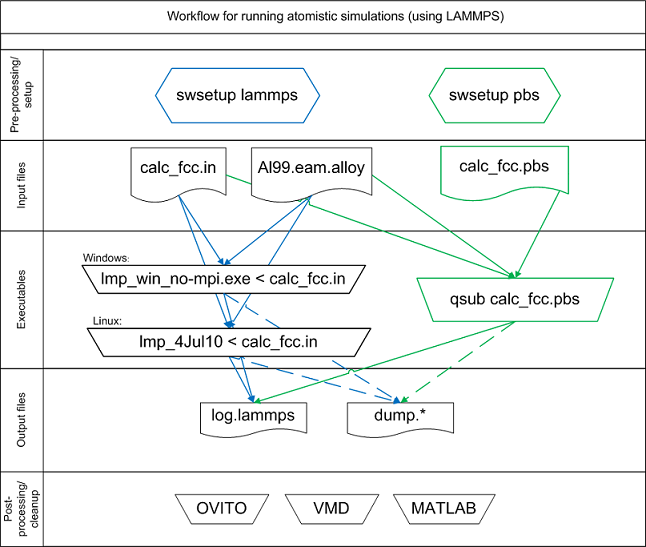
\includegraphics[height=2.50in,width=3.0in, viewport=0 0 646 547,clip]{Figures/Lammps_workflow.png}
\caption{\fontsize{6.2pt}{5.2pt}\selectfont{\textrm{The general workflow for running molecular dynamics simulations using LAMMPS.}}}%(与文献\cite{EPJB33-47_2003}图1对比)
\label{General_Workflow}
\end{figure}
}

\subsection{能量最小化与状态方程}
\frame
{
	\frametitle{\textrm{LAMMPS}的输入参数说明}
	{\fontsize{7.5pt}{6.0pt}\selectfont{
%\verbatiminput{Figures/Lammps_in_lj.txt} %为保险:~选用文件名绝对路径
\verbatiminput{Figures/Lammps_tutorial-01-in_01.txt} %为保险:~选用文件名绝对路径
}
\begin{itemize}
	\item \textcolor{cyan}{\textit{\#}}~开头的部分表示注释,\textrm{LAMMPS}不作任何处理
\end{itemize}
}
\vskip 5pt
%\textrm{LAMMPS}模拟的初始化
{\fontsize{7.5pt}{6.0pt}\selectfont{
%\verbatiminput{Figures/Lammps_in_lj.txt} %为保险:~选用文件名绝对路径
\verbatiminput{Figures/Lammps_tutorial-01-in_02-1.txt} %为保险:~选用文件名绝对路径
\begin{itemize}
	\item \textcolor{cyan}{\textit{clear}}:~清除全部内存信息
	\item \textcolor{cyan}{\textit{unit}}:~设定模拟的单位~ (\textcolor{blue}{\textrm{metal}}~表示选择\textrm{\AA}和\textrm{eV}为单位)
	\item \textcolor{cyan}{\textit{dimension}}:~设定模拟维度~:~\textcolor{blue}{\textrm{3}}~表示三维模拟
	\item \textcolor{cyan}{\textit{boundary}}~\textcolor{blue}{\textrm{p~p~p}}:~表示在$x$-,$y$-,$z$-方向采用周期性边界条件
		\begin{itemize}
{\fontsize{6.2pt}{5.0pt}\selectfont{
			\item \textrm{p}:~周期性边界条件\textrm{(periodic)}
			\item \textrm{f}:~非周期性固定边界条件\textrm{(fixed)}
			\item \textrm{s}:~非周期性包覆边界条件\textrm{(shrink-wrapped)}
			\item \textrm{m}:~非周期性包覆最小值边界条件\textrm{(minimum value)}}}
		\end{itemize}
\end{itemize}
}}
}

\frame
{
	\frametitle{\textrm{LAMMPS}的输入参数说明}
	{\fontsize{7.5pt}{6.0pt}\selectfont{
\verbatiminput{Figures/Lammps_tutorial-01-in_02-2.txt} %为保险:~选用文件名绝对路径
\begin{itemize}
	\item \textcolor{cyan}{\textit{atom\_style}}:~设置计算粒子类型~:~\textcolor{blue}{\textrm{atomic}}表示普通原子类型
		\vskip 4pt
		在反应力场计算中,\textcolor{cyan}{\textit{atom\_style}}选用\textcolor{blue}{\textrm{charge}},而\textcolor{cyan}{\textit{units}}选用\textcolor{blue}{\textrm{full}},即反应力场中需要考虑电荷平衡问题
	\item \textcolor{cyan}{\textit{atom\_modify}}:~\textcolor{blue}{\textrm{map~array}}:~表示设置和定义某些存储原子的属性
	\vskip 4pt
	\textcolor{purple}{语法规则}:~\textcolor{cyan}{\textit{atom\_modify}}:~\textcolor{blue}{\textrm{keyword~value}}
	\vskip 3pt
	\textrm{keyword}:~\textrm{\textcolor{blue}{id}~/~\textcolor{blue}{map}~/~\textcolor{blue}{first}}
		\begin{itemize}
{\fontsize{6.2pt}{5.0pt}\selectfont{
\item \textcolor{blue}{\textrm{id~value}}=\textrm{yes~or~no}:~设置是否储存每一个原子的\textrm{ID}(序号) 默认为~\textrm{yes}
\item \textcolor{blue}{\textrm{map~value}}=\textrm{yes~or~array~or~hash}:~设置如何在需要时具有特定\textrm{ID}的原子被发现(\textrm{array}~比\textrm{hash}~快)
\item \textcolor{blue}{\textrm{first~value}}=\textrm{group~ID}:~\textrm{group~ID}~原子首先出现在内部原子列表中的组}}
		\end{itemize}
		\end{itemize}
	}}
}

\frame
{
	\frametitle{\textrm{LAMMPS}的输入参数说明}
	{\fontsize{7.5pt}{6.0pt}\selectfont{
%\verbatiminput{Figures/Lammps_in_lj.txt} %为保险:~选用文件名绝对路径
\verbatiminput{Figures/Lammps_tutorial-01-in_03.txt} %为保险:~选用文件名绝对路径
}
\begin{itemize}
	\item \textcolor{cyan}{\textit{lattice}}:~设定晶格信息~(可选择的晶格类型有\textrm{sc, fcc, bcc, hcp, diamond}等)、\\
		晶格常数(数值\textrm{4})、晶格矢量方向等
	\item \textcolor{cyan}{\textit{region}}:~设定模拟的原胞,此处设定模拟的名为\textcolor{blue}{\textrm{box}}的\textrm{block}(可以理解为原胞)采用晶格单位,并要求\textrm{box}每个方向的大小取为一个晶格常数
	\item \textcolor{cyan}{\textit{create\_box}}:~使用\textcolor{cyan}{\textit{region}}确定的参数构建模拟的\textrm{box},数量为\textcolor{red}{1个}
	\item \textcolor{cyan}{\textit{replicate}}:~设定每个方向上重复的元胞数目
\end{itemize}
}
}

\frame
{
	\frametitle{\textrm{LAMMPS}的输入参数说明}
%\textrm{LAMMPS}模拟的初始化
{\fontsize{7.5pt}{6.0pt}\selectfont{
%\verbatiminput{Figures/Lammps_in_lj.txt} %为保险:~选用文件名绝对路径
\verbatiminput{Figures/Lammps_tutorial-01-in_04.txt} %为保险:~选用文件名绝对路径
}
\begin{itemize}
	\item \textcolor{cyan}{\textit{pair\_style}}:~设定原子间相互作用(力场)类型,此处势函数的形式为~\textcolor{blue}{\textrm{eam/alloy}}
	\item \textcolor{cyan}{\textit{pair\_coeff}}~\textcolor{blue}{\textrm{$\ast$~$\ast$~Al99.eam.alloy~Al}}:~设定相互作用势(力场)的系数\\
		{\fontsize{6.2pt}{5.2pt}\selectfont{\textcolor{magenta}{势函数(力场)的扩展名提示的是使用相互作用的类型}~\textrm{(eam.alloy~=~eam/alloy)}}}
	\item \textcolor{cyan}{\textit{neighbor}}:~设置表面距离
	\item \textcolor{cyan}{\textit{neigh\_modify}}:~设置原子运动
\end{itemize}
}
}

\frame
{
	\frametitle{\textrm{LAMMPS}的输入参数说明}
	{\fontsize{7.5pt}{6.0pt}\selectfont{
%\verbatiminput{Figures/Lammps_in_lj.txt} %为保险:~选用文件名绝对路径
\verbatiminput{Figures/Lammps_tutorial-01-in_05.txt} %为保险:~选用文件名绝对路径
}
\begin{itemize}
	\item \textcolor{cyan}{\textit{compute}}:~定义计算变量:\\
		\begin{enumerate}
{\fontsize{7.5pt}{5.0pt}\selectfont{
\item \textcolor{purple}{变量\textrm{eng}}:~定义为平均每个原子的势能,并且存储在\textrm{ID:~eng}中
\item \textcolor{purple}{变量\textrm{eatom}}:~定义为求和全部\textcolor{purple}{变量\textrm{eng}}的值:~\textcolor{blue}{\textrm{reduce}}~表示减(负),对\textrm{eng}求和并存储在\textrm{ID:~eatoms}中}}
		\end{enumerate}
\end{itemize}
}
}

\frame
{
	\frametitle{\textrm{LAMMPS}的输入参数说明}
%\vskip 5pt
%\textrm{LAMMPS}模拟的初始化
{\fontsize{7.5pt}{6.0pt}\selectfont{
%\verbatiminput{Figures/Lammps_in_lj.txt} %为保险:~选用文件名绝对路径
\verbatiminput{Figures/Lammps_tutorial-01-in_06.txt} %为保险:~选用文件名绝对路径
}
\begin{itemize}
	\item \textcolor{cyan}{\textit{reset\_timestep}}:~重新设定时间模拟步数\footnote{\fontsize{6.2pt}{5.2pt}\selectfont{\textrm{LAMMPS}模拟中,一般需要设置能量最小化、弛豫、数据采集等阶段,不同阶段模拟步数不同。默认情况下,模拟步数是从模拟开始到模拟结束一直累加计算的}}(此处归零:~\textcolor{blue}{\textrm{0}})
	\item \textcolor{cyan}{\textit{fix}}:~设定\textrm{box/relax},能量最小化过程中对模拟盒施外压,各向同性\textrm{(iso)}都弛豫到\textrm{0.0~Pa}:~\textcolor{blue}{\textrm{vmax}}:~正压压缩,负压膨胀
	\item \textcolor{cyan}{\textit{thermo}}:~每运行\textcolor{blue}{10}次在屏幕上输出一次运行结果
	\item \textcolor{cyan}{\textit{thermo\_style}}:~设定屏幕输出信息
	\item \textcolor{cyan}{\textit{min\_style}}:~设定优化算法(最小化算法),\textcolor{blue}{\textrm{cg}}~指定共轭梯度法
	\item \textcolor{cyan}{\textit{minimize}}:~设定开始最小化过程和最小化收敛精度和最大迭代次数:\\
		其中1,3项为能量最小化,2,4项为能量梯度(力)\\
		(原胞弛豫的模拟由晶格常数为\textrm{4\AA}到\textrm{4.05\AA})
\end{itemize}
}
}

\frame
{
	\frametitle{\textrm{LAMMPS}的输入参数说明}
	{\fontsize{7.5pt}{6.0pt}\selectfont{
%\verbatiminput{Figures/Lammps_in_lj.txt} %为保险:~选用文件名绝对路径
\verbatiminput{Figures/Lammps_tutorial-01-in_07.txt} %为保险:~选用文件名绝对路径
}
\begin{itemize}
	\item \textcolor{cyan}{\textit{natoms}}:~变量定义所有原子数
	\item \textcolor{cyan}{\textit{teng}}:~变量定义总的势能:~\textcolor{blue}{\textrm{teng=eatoms}}
	\item \textcolor{cyan}{\textit{length}}:~变量定义模拟原胞长度:~\textcolor{blue}{\textrm{length=lx}}(模拟盒$x$方向为例)
	\item \textcolor{cyan}{\textit{ecoh}}:~变量定义内聚能:~\textcolor{blue}{\textrm{ecoh=v\_teng/v\_natoms}}\footnote{\fontsize{6.2pt}{5.2pt}\selectfont{同一语句中出现多个变量引用时用\textrm{\textcolor{red}{v}\_variable}表示}}
\end{itemize}}
%\textrm{LAMMPS}模拟的初始化
{\fontsize{7.5pt}{6.0pt}\selectfont{
%\verbatiminput{Figures/Lammps_in_lj.txt} %为保险:~选用文件名绝对路径
\verbatiminput{Figures/Lammps_tutorial-01-in_08.txt} %为保险:~选用文件名绝对路径
}
\begin{itemize}
	\item 设定屏幕输出和\textrm{log}文件的输出变量
	\item \textcolor{red}{\$\{\}}表示定义变量的引用
\end{itemize}
}
}

%\frame[allowframebreaks]
%{
%	\frametitle{\textrm{LAMMPS}的输入文件}
%\fontsize{6.0pt}{5.0pt}\selectfont{
%%\verbatiminput{Figures/Lammps_in_lj.txt} %为保险:~选用文件名绝对路径
%\verbatiminput{Figures/Lammps_tutorial-01-Lammps-in.txt} %为保险:~选用文件名绝对路径
%}
%}
%
\frame
{
	\frametitle{\textrm{LAMMPS}的输出结果}
	\textrm{LAMMPS}执行命令:
	\vskip 5pt
	\textcolor{blue}{lmp}~\textcolor{magenta}{-in}~calc\_fcc.in
	\vskip 5pt
\begin{figure}[h!]
\centering
\vskip -5pt
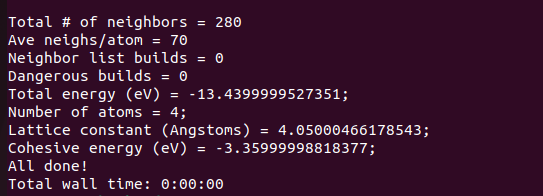
\includegraphics[height=1.50in,width=4.0in, viewport=0 0 543 196,clip]{Figures/Lammps_output.png}
\caption{\fontsize{6.2pt}{5.2pt}\selectfont{\textrm{The end of the logfile/screen output using LAMMPS.}}}%(与文献\cite{EPJB33-47_2003}图1对比)
\label{LAMMPS_output}
\end{figure}
}

%\subsection{状态方程}
\frame[allowframebreaks]
{
	\frametitle{\textrm{LAMMPS}的输入文件}
	{\fontsize{6.0pt}{5.0pt}\selectfont{
%\verbatiminput{Figures/Lammps_in_lj.txt} %为保险:~选用文件名绝对路径
\verbatiminput{Figures/Lammps_tutorial-02-in.txt} %为保险:~选用文件名绝对路径
}}
\textrm{LAMMPS}执行命令~\textcolor{blue}{(指定变量)}:
	\vskip 5pt
	\textcolor{blue}{lmp}~\textcolor{magenta}{-in}~calc\_fcc.in~\textcolor{red}{-var~latconst~4}
}

\frame[allowframebreaks]
{
	\frametitle{\textrm{LAMMPS}的输入文件:~基于\textrm{Matlab}的执行}
	{\fontsize{6.0pt}{5.0pt}\selectfont{
%\verbatiminput{Figures/Lammps_in_lj.txt} %为保险:~选用文件名绝对路径
\verbatiminput{Figures/Lammps_tutorial-02-Lammps-in.txt} %为保险:~选用文件名绝对路径
}}
}

\frame[allowframebreaks]
{
	\frametitle{\textrm{LAMMPS}的输入文件:~基于\textrm{Matlab}的执行}
	{\fontsize{6.0pt}{5.0pt}\selectfont{
%\verbatiminput{Figures/Lammps_in_lj.txt} %为保险:~选用文件名绝对路径
\verbatiminput{Figures/Lammps_tutorial-02-Matlab-in.txt} %为保险:~选用文件名绝对路径
}}
}

\frame[allowframebreaks]
{
	\frametitle{\textrm{LAMMPS}的输入文件:~基于\textrm{Python}的执行}
	{\fontsize{6.0pt}{5.0pt}\selectfont{
%\verbatiminput{Figures/Lammps_in_lj.txt} %为保险:~选用文件名绝对路径
\verbatiminput{Figures/Lammps_tutorial-02-Python-in1.txt} %为保险:~选用文件名绝对路径
}}
}

\frame[allowframebreaks]
{
	\frametitle{\textrm{LAMMPS}的输入文件:~基于\textrm{Python}的执行}
	{\fontsize{6.0pt}{5.0pt}\selectfont{
%\verbatiminput{Figures/Lammps_in_lj.txt} %为保险:~选用文件名绝对路径
\verbatiminput{Figures/Lammps_tutorial-02-Python-in2.txt} %为保险:~选用文件名绝对路径
}}
}

\frame
{
	\frametitle{状态方程}
\begin{figure}[h!]
\centering
\vskip -5pt
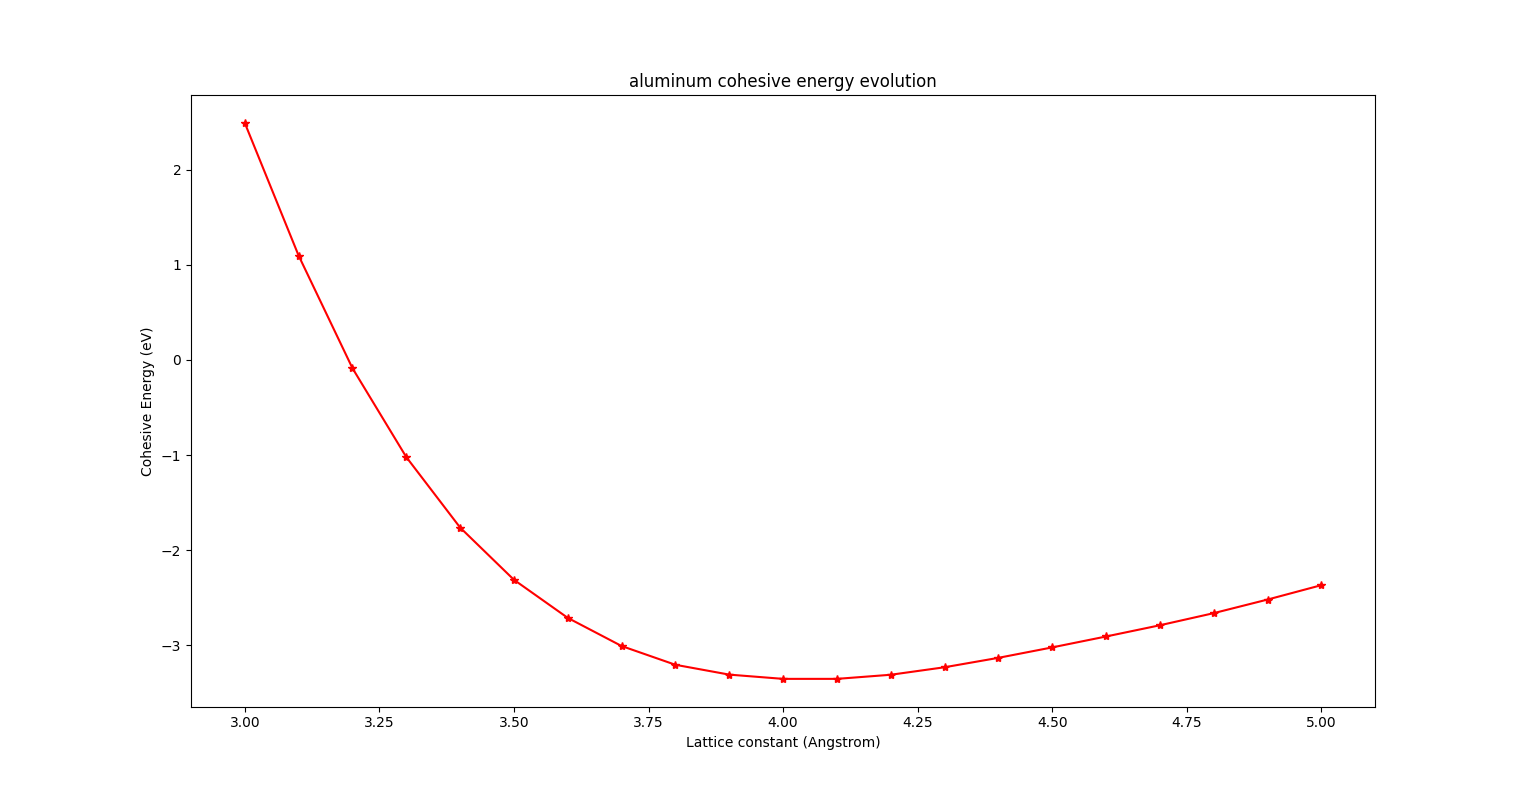
\includegraphics[height=2.50in,width=4.0in, viewport=0 0 1050 554,clip]{Figures/Lammps-EOS.png}
\caption{\fontsize{6.2pt}{5.2pt}\selectfont{\textrm{Aluminum cohesive energy evolution.}}}%(与文献\cite{EPJB33-47_2003}图1对比)
\label{LAMMPS_output-EOS}
\end{figure}
}

\subsection{拉伸与压力下的形变模拟}
\frame[allowframebreaks]
{
	\frametitle{\textrm{LAMMPS}的输入文件}
	{\fontsize{6.0pt}{5.0pt}\selectfont{
%\verbatiminput{Figures/Lammps_in_lj.txt} %为保险:~选用文件名绝对路径
\verbatiminput{Figures/Lammps_tutorial-03-Lammps-in.txt} %为保险:~选用文件名绝对路径
}}
}

\frame[allowframebreaks]
{
	\frametitle{\textrm{LAMMPS}的输入文件:~基于\textrm{Matlab}的执行}
	{\fontsize{6.0pt}{5.0pt}\selectfont{
%\verbatiminput{Figures/Lammps_in_lj.txt} %为保险:~选用文件名绝对路径
\verbatiminput{Figures/Lammps_tutorial-03-Matlab-in.txt} %为保险:~选用文件名绝对路径
}}
}

\frame[allowframebreaks]
{
	\frametitle{\textrm{LAMMPS}的输入文件:~基于\textrm{Python}的执行}
	{\fontsize{6.0pt}{5.0pt}\selectfont{
%\verbatiminput{Figures/Lammps_in_lj.txt} %为保险:~选用文件名绝对路径
\verbatiminput{Figures/Lammps_tutorial-03-Python-in.txt} %为保险:~选用文件名绝对路径
}}
}

\frame
{
	\frametitle{应力-应变曲线}
\begin{figure}[h!]
\centering
\vskip -5pt
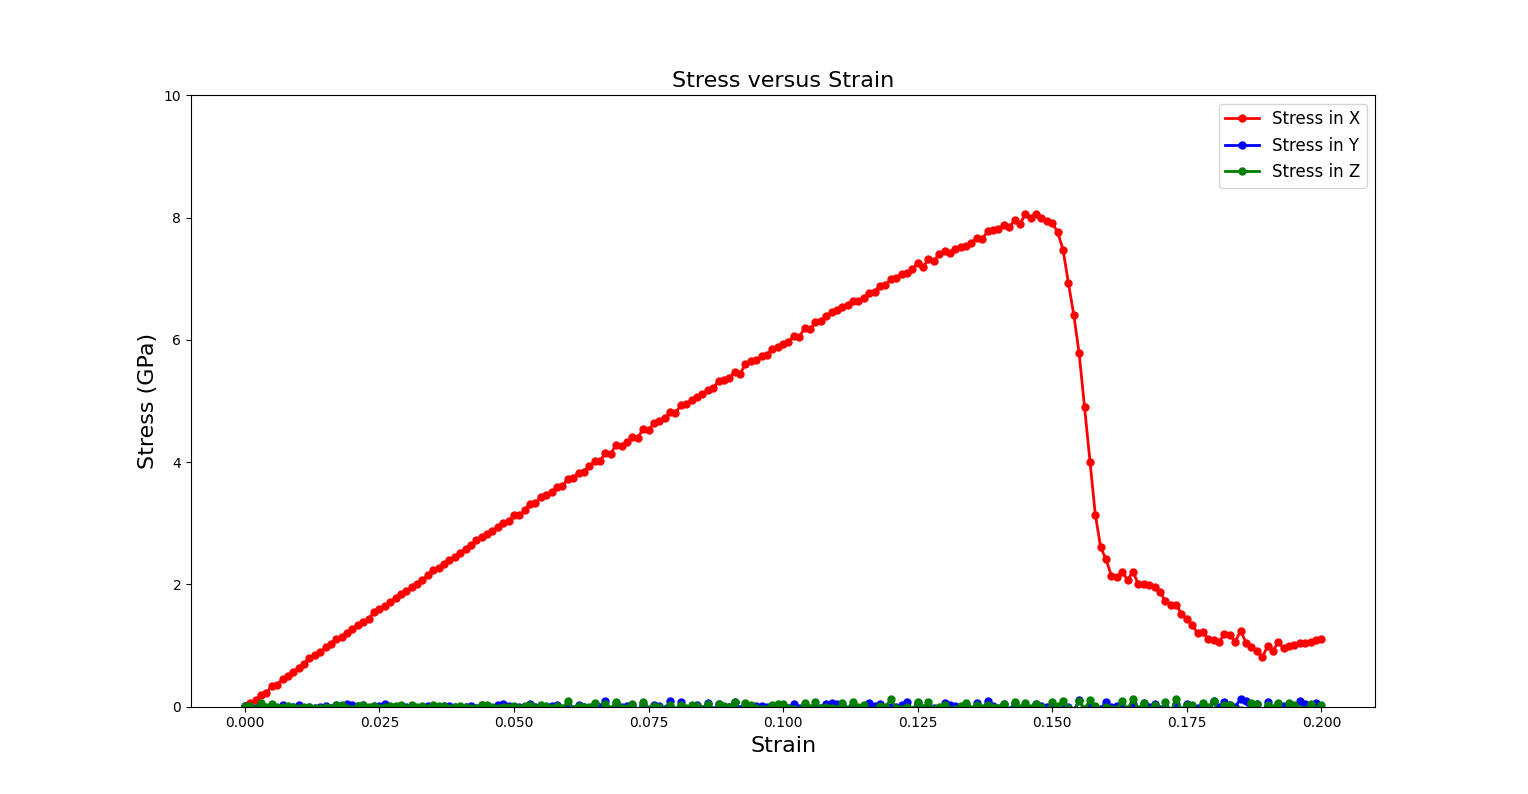
\includegraphics[height=2.20in,width=3.5in, viewport=0 0 1050 554,clip]{Figures/Lammps-Stress_Strain.png}
\caption{\fontsize{6.2pt}{5.2pt}\selectfont{\textrm{Stress-strain curve for uniaxial tensile loading of single crystal aluminum in the <100> loading direction.}}}%(与文献\cite{EPJB33-47_2003}图1对比)
\label{LAMMPS_output-Stress-Strain}
\end{figure}
}

\frame
{
	\frametitle{拉伸载荷}
\begin{figure}[h!]
\centering
\vskip -5pt
\animategraphics[autoplay, loop, height=2.40in, width=2.50in,viewport= 0 0 256 256,clip]{1}{Figures/Lammps-simulation-cell-in-tension-}{0}{81}
\caption{\fontsize{6.2pt}{5.2pt}\selectfont{\textrm{Tensile Loading of an Aluminum Single Crystal..}}}%(与文献\cite{EPJB33-47_2003}图1对比)
\label{LAMMPS_Tensile-Loading}
\end{figure}
}

\frame[allowframebreaks]
{
	\frametitle{\textrm{LAMMPS}的输入文件}
	{\fontsize{6.0pt}{5.0pt}\selectfont{
%\verbatiminput{Figures/Lammps_in_lj.txt} %为保险:~选用文件名绝对路径
\verbatiminput{Figures/Lammps_tutorial-04-Lammps-in.txt} %为保险:~选用文件名绝对路径
}}
}

\frame
{
	\frametitle{应力-应变曲线}
\begin{figure}[h!]
\centering
\vskip -5pt
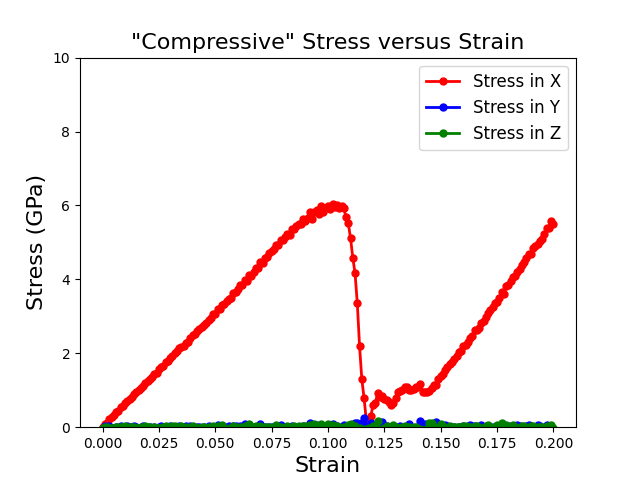
\includegraphics[height=2.40in,width=3.0in, viewport=0 0 450 354,clip]{Figures/Lammps-Compressive-Stress_Strain.png}
\caption{\fontsize{6.2pt}{5.2pt}\selectfont{\textrm{Compressive Stress-strain curve for uniaxial compression loading of single crystal aluminum in the <100> loading direction.}}}%(与文献\cite{EPJB33-47_2003}图1对比)
\label{LAMMPS_output-Stress-Strain}
\end{figure}
}

\frame
{
	\frametitle{压缩载荷}
\begin{figure}[h!]
\centering
\vskip -5pt
\animategraphics[autoplay, loop, height=2.40in, width=2.50in,viewport= 0 0 256 256,clip]{1}{Figures/Lammps-simulation-cell-in-compression-}{0}{80}
\caption{\fontsize{6.2pt}{5.2pt}\selectfont{\textrm{Compression Loading of an Aluminum Single Crystal.}}}%(与文献\cite{EPJB33-47_2003}图1对比)
\label{LAMMPS_Compression-Loading}
\end{figure}
}

\subsection{模拟晶界的形成}
\frame[allowframebreaks]
{
	\frametitle{\textrm{LAMMPS}的输入文件}
	{\fontsize{6.0pt}{5.0pt}\selectfont{
%\verbatiminput{Figures/Lammps_in_lj.txt} %为保险:~选用文件名绝对路径
\verbatiminput{Figures/Lammps_tutorial-05-Lammps-in.txt} %为保险:~选用文件名绝对路径
}}
}

\frame
{
	\frametitle{\textrm{LAMMPS}的输出文件}
\begin{figure}[h!]
\centering
\vskip -10pt
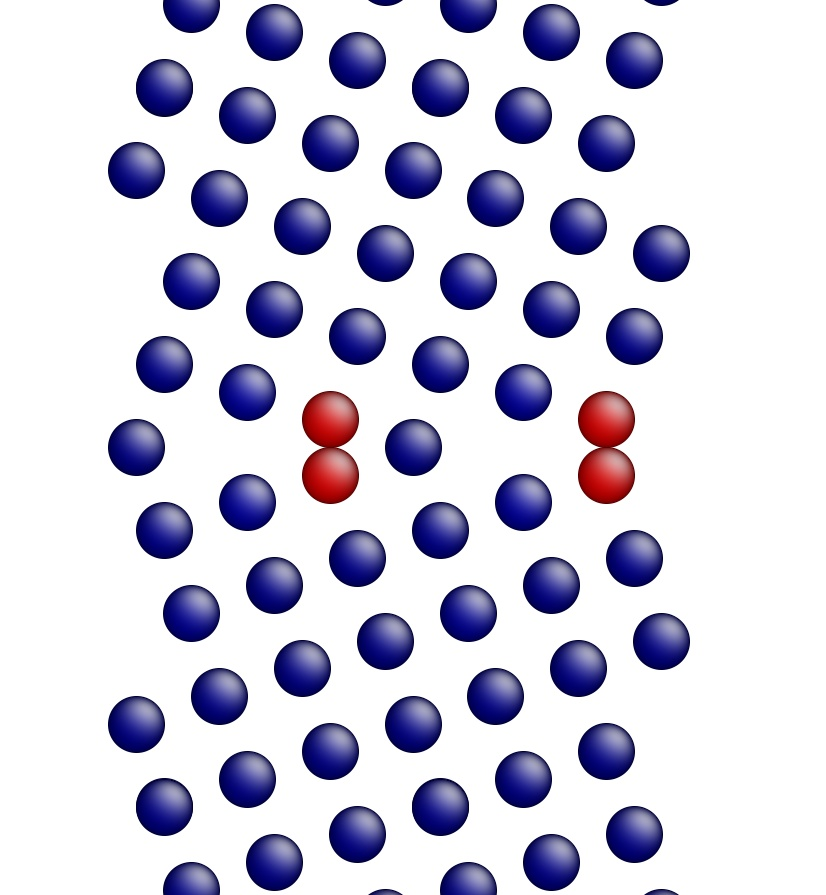
\includegraphics[height=2.40in,width=2.3in, viewport=0 0 780 890,clip]{Figures/Lammps-simulation_grain_boundary_structure-1.jpeg}
\caption{\fontsize{6.2pt}{5.2pt}\selectfont{\textrm{The grain boundary structure prior to minimization.}}}%(与文献\cite{EPJB33-47_2003}图1对比)
\label{LAMMPS_output-simulation_grain_boundary_structure-1}
\end{figure}
}

\frame
{
	\frametitle{\textrm{LAMMPS}的输出文件}
\begin{figure}[h!]
\centering
\vskip -10pt
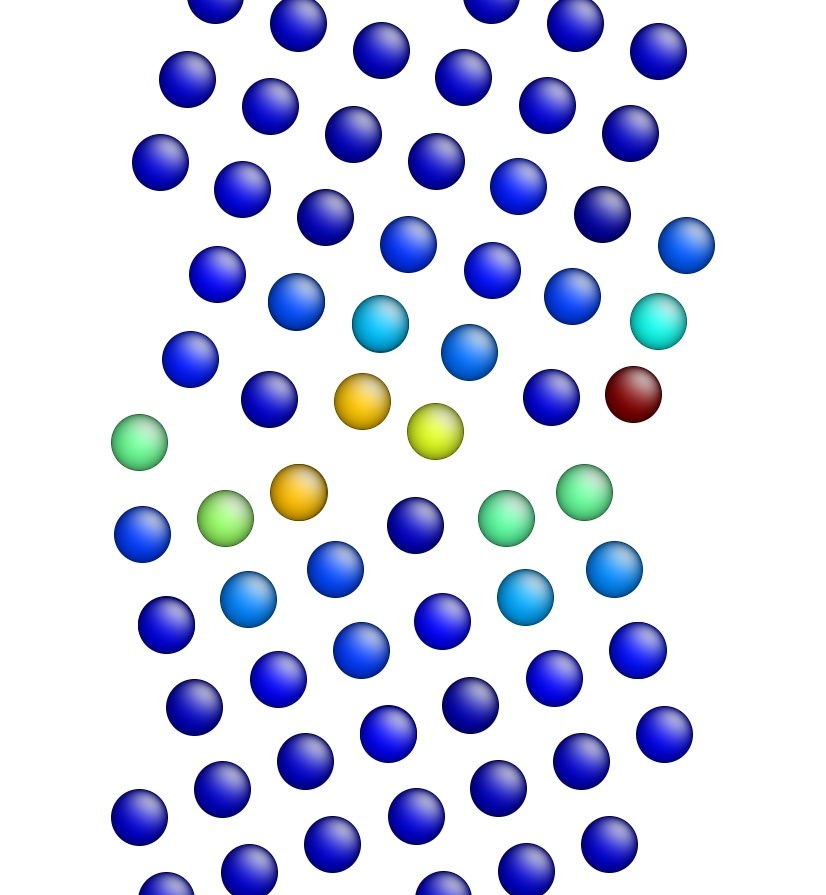
\includegraphics[height=2.40in,width=2.3in, viewport=0 0 780 890,clip]{Figures/Lammps-simulation_grain_boundary_structure-2.jpeg}
\caption{\fontsize{6.2pt}{5.2pt}\selectfont{\textrm{The grain boundary structure after minimization (overlap distance equals 0.35).}}}%(与文献\cite{EPJB33-47_2003}图1对比)
\label{LAMMPS_output-simulation_grain_boundary_structure-2}
\end{figure}
}

\frame
{
	\frametitle{\textrm{LAMMPS}的输出文件}
\begin{figure}[h!]
\centering
\vskip -10pt
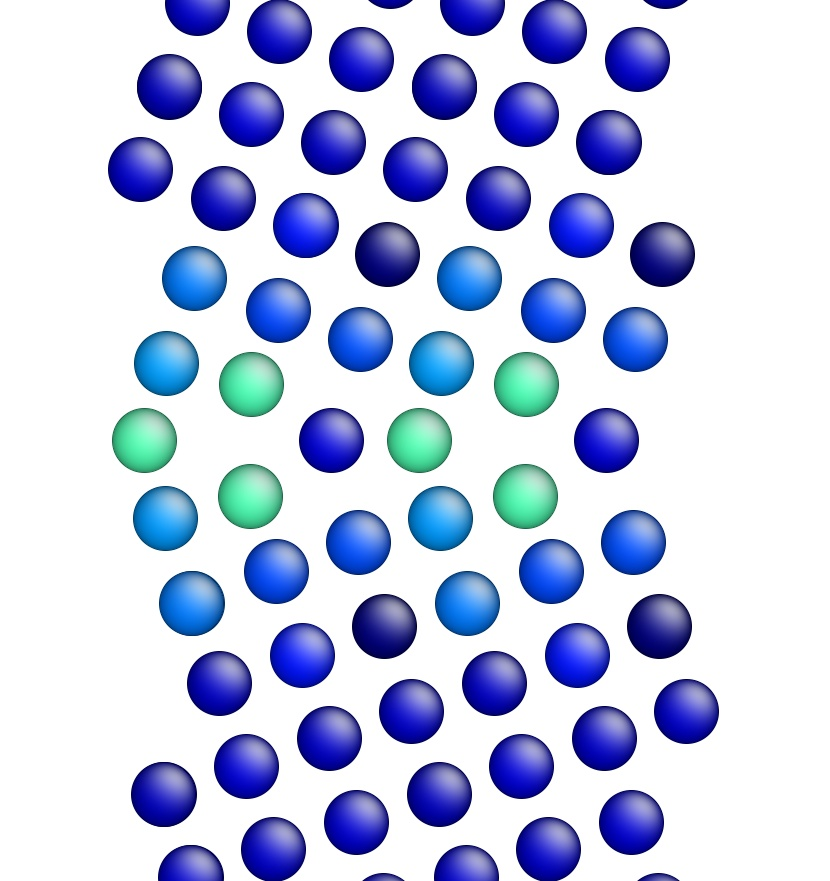
\includegraphics[height=2.40in,width=2.3in, viewport=0 0 780 890,clip]{Figures/Lammps-simulation_grain_boundary_structure-3.jpeg}
\caption{\fontsize{6.2pt}{5.2pt}\selectfont{\textrm{The grain boundary structure after minimization (overlap distance equals 1.50).}}}%(与文献\cite{EPJB33-47_2003}图1对比)
\label{LAMMPS_output-simulation_grain_boundary_structure-3}
\end{figure}
}

\frame
{
	\frametitle{\textrm{LAMMPS}的输出文件}
\begin{figure}[h!]
\centering
\vskip -10pt
\animategraphics[autoplay, loop, height=2.40in, width=2.00in,viewport= 0 0 400 470,clip]{1}{Figures/Lammps-simulation_grain_boundary-for-aluminum-1-}{0}{31}
\caption{\fontsize{6.2pt}{5.2pt}\selectfont{\textrm{The minimization of the grain boundary structure for an aluminum $\Sigma5(310)$ symmetric tilt grain boundary.}}}%(与文献\cite{EPJB33-47_2003}图1对比)
\label{LAMMPS_output-simulation_fracture-of-Fe}
\end{figure}
}

\frame
{
	\frametitle{\textrm{LAMMPS}的输出文件}
\begin{figure}[h!]
\centering
\vskip -10pt
\animategraphics[autoplay, loop, height=2.40in, width=2.00in,viewport= 0 0 400 470,clip]{1}{Figures/Lammps-simulation_grain_boundary-for-aluminum-2-}{0}{16}
\caption{\fontsize{6.2pt}{5.2pt}\selectfont{\textrm{The minimization of the grain boundary structure for an aluminum $\Sigma5(310)$ symmetric tilt grain boundary (with a slightly different starting position.).}}}%(与文献\cite{EPJB33-47_2003}图1对比)
\label{LAMMPS_output-simulation_fracture-of-Fe}
\end{figure}
}

\subsection{拉伸晶界直至断裂}
\frame[allowframebreaks]
{
	\frametitle{\textrm{LAMMPS}的输入文件}
	{\fontsize{6.0pt}{5.0pt}\selectfont{
%\verbatiminput{Figures/Lammps_in_lj.txt} %为保险:~选用文件名绝对路径
\verbatiminput{Figures/Lammps_tutorial-06-Lammps-in.txt} %为保险:~选用文件名绝对路径
}}
}

\frame
{
	\frametitle{\textrm{LAMMPS}的输出文件}
\begin{figure}[h!]
\centering
\vskip -10pt
\animategraphics[autoplay, loop, height=2.40in, width=1.10in,viewport= 30 0 170 260,clip]{1}{Figures/Lammps-simulation_fracture-of-Fe-}{0}{120}
\caption{\fontsize{6.2pt}{5.2pt}\selectfont{\textrm{The fracture of a Fe symmetric tilt grain boundary. Atoms are colored by the stress in the y-direction.}}}%(与文献\cite{EPJB33-47_2003}图1对比)
\label{LAMMPS_output-simulation_fracture-of-Fe}
\end{figure}
}

\subsection{铁的对称倾转晶界断裂的原子模拟}
\frame[allowframebreaks]
{
	\frametitle{\textrm{LAMMPS}的输入文件}
	{\fontsize{6.0pt}{5.0pt}\selectfont{
%\verbatiminput{Figures/Lammps_in_lj.txt} %为保险:~选用文件名绝对路径
\verbatiminput{Figures/Lammps_tutorial-07-Lammps-in.txt} %为保险:~选用文件名绝对路径
}}
}

\frame[allowframebreaks]
{
	\frametitle{\textrm{LAMMPS}的\textrm{data}文件}
	{\fontsize{6.0pt}{5.0pt}\selectfont{
%\verbatiminput{Figures/Lammps_in_lj.txt} %为保险:~选用文件名绝对路径
\verbatiminput{Figures/Lammps_tutorial-07-Lammps-data.txt} %为保险:~选用文件名绝对路径
}}
}

\frame
{
	\frametitle{\textrm{LAMMPS}的输出文件}
\begin{figure}[h!]
\centering
\vskip -5pt
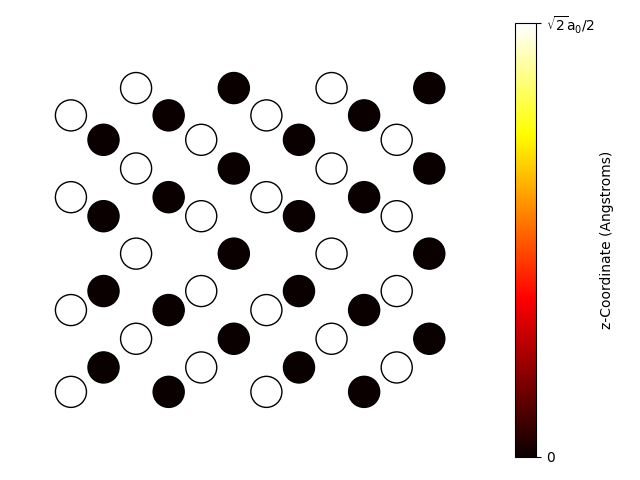
\includegraphics[height=2.40in,width=3.4in, viewport=0 0 450 354,clip]{Figures/Lammps-grain_boundary-for-atoms-1.png}
\caption{\fontsize{6.2pt}{5.2pt}\selectfont{\textrm{The atoms colored by the in-plane coordinate (z-direction:~the black and white grain boundary structure look for atoms that sit on different \{110\} planes).}}}%(与文献\cite{EPJB33-47_2003}图1对比)
\label{LAMMPS_output-grain_boundary-for-atoms-1}
\end{figure}
}

%\frame
%{
%	\frametitle{\textrm{LAMMPS}的输出文件}
%\begin{figure}[h!]
%\centering
%\vskip -5pt
%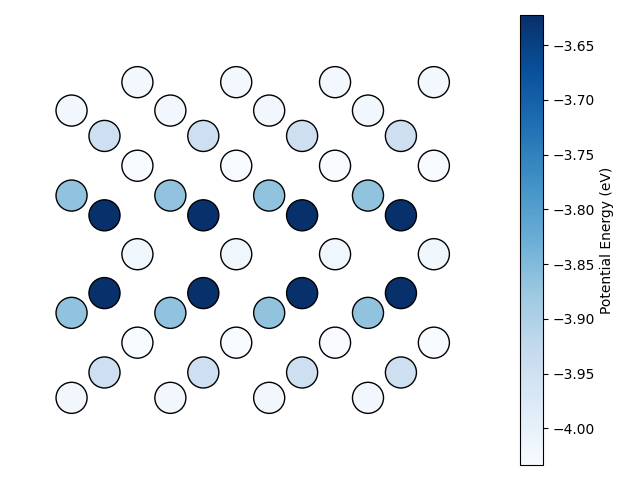
\includegraphics[height=2.40in,width=3.0in, viewport=0 0 450 354,clip]{Figures/Lammps-grain_boundary-for-atoms-2.png}
%\caption{\fontsize{6.2pt}{5.2pt}\selectfont{\textrm{The atoms colored by the in-plane coordinate (z-direction:~the black and white grain boundary structure look for atoms that sit on different \{110\} planes).}}}%(与文献\cite{EPJB33-47_2003}图1对比)
%\label{LAMMPS_output-grain_boundary-for-atoms-2}
%\end{figure}
%}
%
\subsection{长链聚合物行为模拟}
\frame[allowframebreaks]
{
	\frametitle{\textrm{LAMMPS}的\textrm{data}文件}
	{\fontsize{6.0pt}{5.0pt}\selectfont{
%\verbatiminput{Figures/Lammps_in_lj.txt} %为保险:~选用文件名绝对路径
\verbatiminput{Figures/Lammps_tutorial-08-Lammps-data.txt} %为保险:~选用文件名绝对路径
}}
}

\frame
{
	\frametitle{\textrm{LAMMPS}中的键角与二面角}
\begin{figure}[h!]
\centering
\vskip -5pt
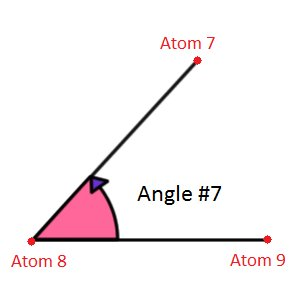
\includegraphics[height=1.70in,width=1.9in, viewport=0 0 320 280,clip]{Figures/Lammps-Angles_between_atoms.jpeg}
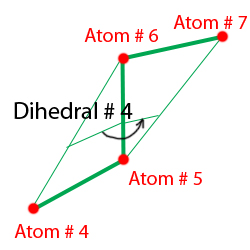
\includegraphics[height=1.70in,width=1.9in, viewport=0 0 280 250,clip]{Figures/Lammps-Dihedral_angles_between_atoms.jpeg}
\caption{\fontsize{6.2pt}{5.2pt}\selectfont{\textrm{A schematic of angles~(left) and dihedral angles~(right) between atoms defined in LAMMPS.}}}%(与文献\cite{EPJB33-47_2003}图1对比)
\label{LAMMPS_Angle-and-Dihedral_angle}
\end{figure}
}

\frame[allowframebreaks]
{
	\frametitle{\textrm{LAMMPS}的输入文件}
	{\fontsize{6.0pt}{5.0pt}\selectfont{
%\verbatiminput{Figures/Lammps_in_lj.txt} %为保险:~选用文件名绝对路径
\verbatiminput{Figures/Lammps_tutorial-08-Lammps-in.txt} %为保险:~选用文件名绝对路径
}}
}

\frame
{
	\frametitle{\textrm{LAMMPS}的输出文件}
\begin{figure}[h!]
\centering
\vskip -5pt
\animategraphics[autoplay, loop, height=2.40in, width=2.50in,viewport= 0 0 556 536,clip]{1}{Figures/Lammps-simulation_Equilibration-process-followed-by-minimization-}{0}{211}
\caption{\fontsize{6.2pt}{5.2pt}\selectfont{\textrm{Equilibration process followed by minimization for a single polymer chain.}}}%(与文献\cite{EPJB33-47_2003}图1对比)
\label{LAMMPS_output-Equilibration-process-followed-by-minimization}
\end{figure}
}
%\vskip 5pt
%------------------------------------------------------------------------Reference----------------------------------------------------------------------------------------------
		\frame[allowframebreaks]
{
\frametitle{主要参考文献}
\begin{thebibliography}{99}
{\tiny
	\bibitem{url_lammps-tutorials}\url{https://github.com/mrkllntschpp/lammps-tutorials}
		\vskip 2pt \textcolor{magenta}{\fontsize{5.2pt}{5.2pt}\selectfont{(\textrm{LAMMPS}基本计算出处)}}
	\bibitem{J.-G._Lee}\textrm{J.-G. Lee, \textit{Computational Materials Science:~an introduction}}~\textrm{(2nd Edition),~CPC Press}, \textrm{(2017)}
		\vskip 2pt \textcolor{magenta}{\fontsize{5.2pt}{5.2pt}\selectfont{(\textrm{LAMMPS}模型算例出处)}}
%	\bibitem{url_Atom-Eye}\url{http://li.mit.edu/Archive/Graphics/A/}
		\vskip 8pt \textcolor{blue}{\textrm{LAMMPS}常用的可视化软件:}
\bibitem{url_Atom-Eye_download}\url{http://li.mit.edu/Archive/Graphics/A/#download}
%\bibitem{url_ImageJ}\url{https://imagej.net/ij/}
\bibitem{url_ImageJ_download}\url{https://imagej.net/ij/download.html}
\bibitem{url_ovito_download}\url{https://www.ovito.org/os-downloads/}
\bibitem{url_VMD_download}\url{https://www.ks.uiuc.edu/Development/Download/download.cgi?PackageName=VMD}
}
\end{thebibliography}
}
\frame
{
	\frametitle{材料计算软件发展现状}
\begin{figure}[h!]
\vspace*{-0.16in}
\centering

\includegraphics[width=3.30in]{Figures/Softwares_logo.png}
%\caption{\tiny \textrm{Pseudopotential for metallic sodium, based on the empty core model and screened by the Thomas-Fermi dielectric function.}}%(与文献\cite{EPJB33-47_2003}图1对比)
\label{Softwares}
\end{figure}
}

\frame
{
	\frametitle{国产第一原理计算软件现状}
\begin{figure}[h!]
\vspace*{-0.19in}
\centering
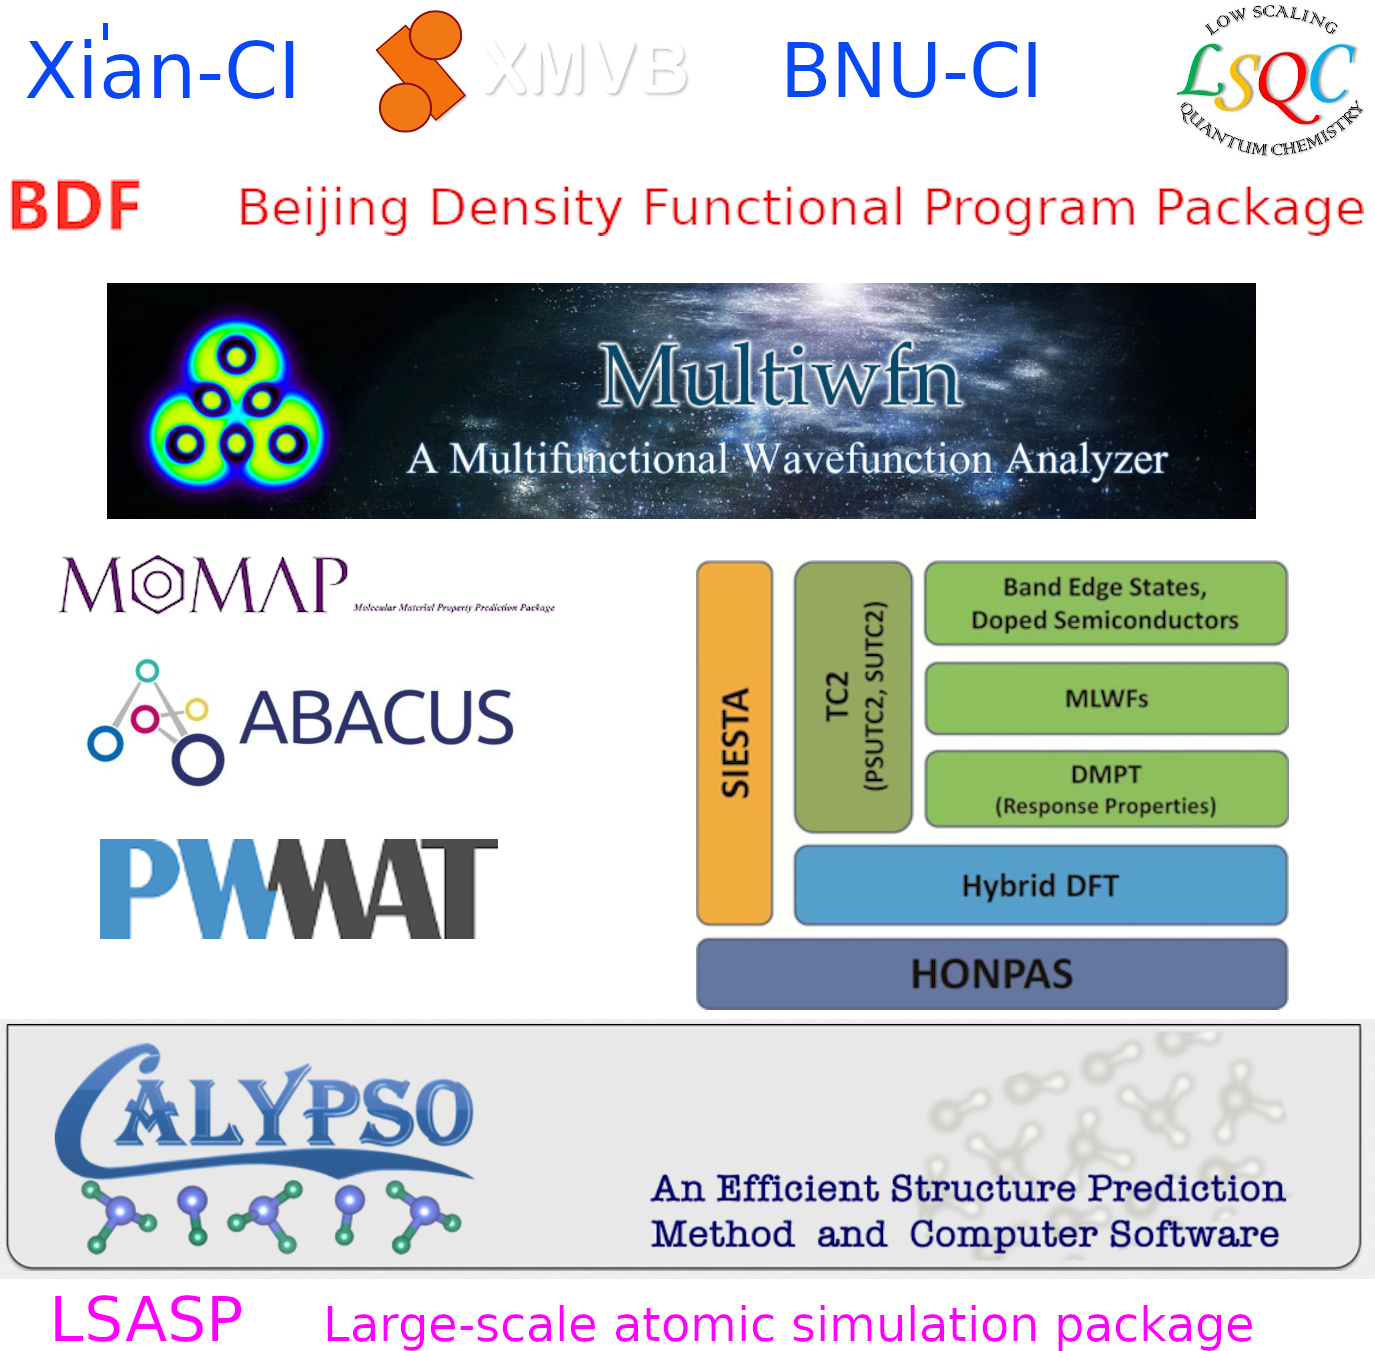
\includegraphics[width=2.83in]{Figures/Softwares_China-logo.png}
%\caption{\tiny \textrm{Pseudopotential for metallic sodium, based on the empty core model and screened by the Thomas-Fermi dielectric function.}}%(与文献\cite{EPJB33-47_2003}图1对比)
\label{Software-China}
\end{figure}
	\fontsize{6.2pt}{5.2pt}\selectfont{\textcolor{red}{中国学科发展战略\,$\cdot$\,理论与计算化学,~~国家自然科学基金委员会,~中国科学院,~~北京:~科学出版社,~~2016}}
}

\appendix
\section{高通量材料计算平台开发现状}     %Bookmark
\frame
{
	\frametitle{国内已有的计算平台:~\textrm{MatCloud}}
\begin{figure}[h!]:
\centering

\includegraphics[height=1.57in,width=4.95in,viewport=0 0 1800 550,clip]{Figures/Matcloud-login.png}
\caption{\fontsize{7.2pt}{4.2pt}\selectfont{中科院计算机网络信息中心~杨小渝团队开发}\upcite{CMS146-319_2018,url_Matcloud}}%
\label{Auto_Flow_Platform-2}
\end{figure}
}

\frame
{
	\frametitle{国外已有的计算平台}
\begin{figure}[h!]
\centering
\vspace{-15.5pt}
\subfigure[\fontsize{7.5pt}{6.2pt}\selectfont{\textrm{Auto-FLOW (AFLOW)}\upcite{CMS58-227_2012}}]{
\label{AFLOW_data_flow}
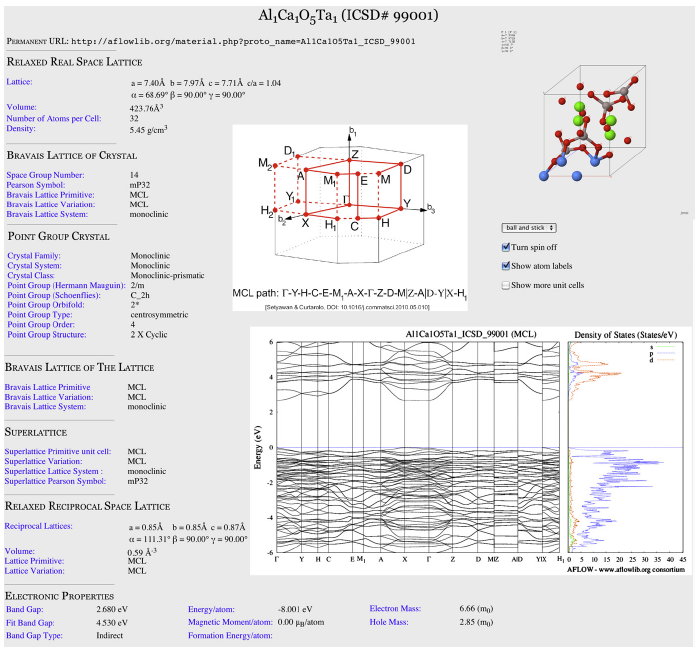
\includegraphics[height=1.2in,width=1.6in,viewport=0 0 720 660,clip]{Figures/AFLOW_database.png}}
\subfigure[\fontsize{7.5pt}{6.2pt}\selectfont{\textrm{Material Project (MP)}\upcite{CMS97-209_2015}}]{
\label{MP_commp_infrastructure}
\includegraphics[height=1.2in,width=1.7in,viewport=0 0 670 530,clip]{Figures/MP_comp_infrastructure.png}}
\subfigure[\fontsize{3.5pt}{3.2pt}\selectfont{\textrm{Quantum Materials Informatics Project (QMIP)}\upcite{url_QMIP}}]{
\label{QMIP_Shame}
\includegraphics[height=1.2in,width=1.7in,viewport=0 0 670 420,clip]{Figures/QMIP_shame.png}}
\subfigure[\fontsize{6.5pt}{5.2pt}\selectfont{\textrm{Clean Energy Project (CEP)}\upcite{JPCL2-2241_2011}}]{
\label{CEP_structure_flow}
\includegraphics[height=1.2in,width=1.6in,viewport=0 0 1020 730,clip]{Figures/CEP_structure_flow.png}}
%\caption{}%
\label{Auto_Flow_Platform-1}
\end{figure}
}

\frame
{
	\frametitle{\textrm{ASE}:~接口丰富的适应性计算平台}
\begin{figure}[h!]
\centering
\vspace*{-0.2in}
\includegraphics[height=2.1in,width=3.2in,viewport=0 0 1208 830,clip]{Figures/ASE_Python_lib.png}
\caption{\fontsize{7.2pt}{4.2pt}\selectfont{\textrm{ASE:~a Python library for working with atoms.}}}%
\label{Logo_ASE_lib}
\end{figure} 
}

\frame
{
	\frametitle{\textrm{Atomly}:~物理所的无机晶体材料计算数据库}
\begin{figure}[h!]
\centering
\vspace*{-0.2in}
\includegraphics[height=2.1in,width=4.1in,viewport=5 0 1608 830,clip]{Figures/Atomly.png}
\caption{\fontsize{7.2pt}{4.2pt}\selectfont{\textrm{Atomly:~中科院物理所~刘淼等老师开发,数据库包含了17万\!$^+$\!无机晶体材料第一性原理计算结果\textrm{(包含电子结构信息:~DOS~+~energy~bands)}.}}}%
\label{Logo_Atomly_lib}
\end{figure} 
}

\frame
{
	\frametitle{\textrm{计算平台的功能和总体架构}}
\begin{figure}[h!]
\centering
\vspace*{-0.35in}
\includegraphics[height=2.6in,width=4.05in,viewport=0 0 670 460,clip]{Figures/Parallel_computation.png}
%\includegraphics[height=1.6in,width=2.4in,viewport=0 0 1038 730,clip]{Figures/Auto_Flow.png}
\caption{\fontsize{7.2pt}{4.2pt}\selectfont{\textrm{The schematic framework and platform of all those project.}}}%
\label{Auto_Flow}
\end{figure} 
}

\frame
{
	\frametitle{现有高通量计算平台概览}
\begin{table}[!h]
\tabcolsep 0pt \vspace*{-12pt}
%\caption{}
\label{Table-Cost}
\begin{minipage}{0.85\textwidth}
%\begin{center}
\centering
\def\temptablewidth{1.1\textwidth}
\renewcommand\arraystretch{0.8} %表格宽度控制(普通表格宽度的两倍)
\rule{\temptablewidth}{1pt}
\begin{tabular*} {\temptablewidth}{@{\extracolsep{\fill}}c@{\extracolsep{\fill}}c@{\extracolsep{\fill}}c@{\extracolsep{\fill}}c@{\extracolsep{\fill}}c@{\extracolsep{\fill}}c@{\extracolsep{\fill}}c}
%-------------------------------------------------------------------------------------------------------------------------
	&\multirow{2}{*}{\fontsize{7.2pt}{5.2pt}\selectfont{编程语言}}	&\fontsize{7.2pt}{5.2pt}\selectfont{建模} &\multicolumn{2}{|c|}{\fontsize{6.2pt}{5.2pt}\selectfont{任务提交与管理}} &\multirow{2}{*}{\fontsize{7.2pt}{5.2pt}\selectfont{后处理}} &\multirow{2}{*}{\fontsize{6.2pt}{5.2pt}\selectfont{数据组织管理}} \\\cline{4-5}
	&	&\fontsize{7.2pt}{5.2pt}\selectfont{功能} &\multicolumn{1}{|l}{\fontsize{7.2pt}{5.2pt}\selectfont{软件接口}} &\multicolumn{1}{r|}{\fontsize{7.2pt}{5.2pt}\selectfont{运行容错}} & & \\\hline
	\fontsize{7.2pt}{5.2pt}\selectfont{{AFLOW}} &\fontsize{7.2pt}{5.2pt}\selectfont{C++} &\checkmark &$\triangle$ &\FiveStarOpen &\FiveStarOpen &\fontsize{7.2pt}{5.2pt}\selectfont{{Django}} \\
	\fontsize{7.2pt}{5.2pt}\selectfont{{MP}} &\fontsize{7.2pt}{5.2pt}\selectfont{Python} &\checkmark &\checkmark &\FiveStarOpen &\FiveStarOpen &\fontsize{7.2pt}{5.2pt}\selectfont{{MongoDB}} \\
	\multirow{2}{*}{\fontsize{7.2pt}{5.2pt}\selectfont{{QMIP}}} &\fontsize{7.2pt}{5.2pt}\selectfont{JavaScript/SVG} &\multirow{2}{*}{\checkmark} &\multirow{2}{*}{\checkmark} &\multirow{2}{*}{--} &\multirow{2}{*}{\checkmark} &\multirow{2}{*}{--} \\
	&\fontsize{7.2pt}{5.2pt}\selectfont{+html/Python} & & & & & \\
	\fontsize{7.2pt}{5.2pt}\selectfont{{CEP}} &\fontsize{7.2pt}{5.2pt}\selectfont{Python} &\checkmark &\checkmark &-- &\checkmark &\fontsize{7.2pt}{5.2pt}\selectfont{{Django/MySQL}} \\
	\fontsize{7.2pt}{5.2pt}\selectfont{{ASE}} &\fontsize{7.2pt}{5.2pt}\selectfont{Python} &\FiveStarOpen &\FiveStarOpen &-- &$\triangle$ &-- \\
	\multirow{2}{*}{\fontsize{7.2pt}{5.2pt}\selectfont{{MatCloud}}} &\fontsize{7.2pt}{5.2pt}\selectfont{JavaScript} &\multirow{2}{*}{\checkmark} &\multirow{2}{*}{$\triangle$} &\multirow{2}{*}{\checkmark} &\multirow{2}{*}{\checkmark} &\multirow{2}{*}{\fontsize{7.2pt}{5.2pt}\selectfont{{MongoDB}}} \\
	&\fontsize{7.2pt}{5.2pt}\selectfont{+.NETCore} & & & & &
\end{tabular*}
\rule{\temptablewidth}{1pt}
\end{minipage}
%\vskip -15pt
\fontsize{7.2pt}{5.2pt}\selectfont{
\begin{description}
	\item[\FiveStarOpen]~该功能较突出
	\item[\checkmark]~该功能基本满足需求
	\item[$\triangle$]~该功能存在不足
\end{description}}
%\end{center}
\end{table}
\fontsize{8.2pt}{6.2pt}\selectfont{
	\textrm{Lin L. \textit{Materials databases infrastructure constructed by first principles calculations:~a review.} \textbf{Mater. Perform. Character.}, 2015, 4(1):148.}}
}

\subsection{\rm{MP}与\rm{ASE}}     %Bookmark
\frame
{
	\frametitle{\textrm{MP}自动流程的设计与开发}
	\begin{itemize}
		\item \textcolor{red}{设计目标}:~围绕\textrm{VASP~}作业高通量并发提交与过程监控
		\item \textcolor{red}{设计方案}:~开发针对不同计算场景的功能模块
			\begin{enumerate}
    \setlength{\itemsep}{15pt}
				\item \textcolor{blue}{\textbf{Pymatgen}}\\
					\textcolor{magenta}{前处理}:~计算模型的分析与预处理\\
					\textcolor{magenta}{后处理}:~计算结果的可视化
				\item \textcolor{blue}{\textbf{FireWorks}}\\
\textcolor{magenta}{计算流程设计与管理}:~数据库支持的计算流程管理
				\item \textcolor{blue}{\textbf{Custodian}}\\
\textcolor{magenta}{计算流程容错与应对}:~提供计算过程错误判断接口,由用户提供解决策略和针对性设计
			\end{enumerate}
	\end{itemize}
		%\item 计算过程的控制方式
}

\frame
{
	\frametitle{\textrm{Pymatgen}的模块结构}
\begin{figure}[h!]
\centering
\vspace*{-0.1in}
\includegraphics[height=2.3in]{Figures/MP_library.png}
\caption{\fontsize{7.2pt}{4.2pt}\selectfont{\textrm{Overview of a typical workflow for pymatgen.}}}%
\label{Pymatgen_Lib}
\end{figure} 
}

\frame
{
	\frametitle{\textrm{Pymatgen}可展示的材料物性}
\begin{figure}[h!]
\centering
\vspace*{-0.1in}
\includegraphics[height=2.3in]{Figures/MP_vision.png}
\caption{\fontsize{5.2pt}{4.2pt}\selectfont{\textrm{Top left: Phase; Top right: Pourbaix diagram from the Materials API. \\Bottom left: Calculated bandstructure plot using pymatgen’s parsing and plotting utilities. Bottom right: Arrhenius plot using pymatgen’s Diffusion~Analyzer.}}}%
\label{Pymatgen_vision}
\end{figure} 
}

\frame
{
	\frametitle{\textrm{FireWorks}的模块结构}
\textrm{FireWorks}发布的工作流成由三层嵌套结构组成:
\fontsize{8.2pt}{6.2pt}\selectfont{
\begin{itemize}
	\item \textrm{Firetask}:~基本执行单元,是执行计算的最基本脚本命令或\textrm{Python}命令。
	\item \textrm{Firework}:~组织基本执行单元构成任务单元组,并指定各基本执行单元所需的参数。
	\item \textrm{Workflow}:~彼此相关联的任务单元组构成完整的工作流程:\\
		\textrm{FireWork}之间的数据传递、任务执行序列等由\textrm{FWAction}完成。
\end{itemize}}
\begin{figure}[h!]
\centering
\vspace*{-0.1in}
\includegraphics[height=1.5in]{Figures/MP_fireworks.png}
\hskip 1pt
\includegraphics[height=1.5in]{Figures/MP_multiple_fw.png}
\caption{\fontsize{7.2pt}{4.2pt}\selectfont{\textrm{The basic infrastructure of FireWorks.}}}%
\label{FireWorks_FW}
\end{figure} 
}

\frame
{
	\frametitle{\textrm{atomate}:~计算流程控制示范}
%		\textcolor{purple}{\textrm{Atomate}}:~:~适合一定复杂程度的\textrm{~VASP~}计算
\begin{figure}[h!]
\centering
\vspace*{-0.19in}
\includegraphics[height=1.4in,width=2.2in,viewport=0 0 820 630,clip]{Figures/Atomate_comp.png}
\vskip 1pt
\includegraphics[height=1.5in]{Figures/bandstructure_wf.png}
%\caption{\fontsize{7.2pt}{4.2pt}\selectfont{\textrm{The integrated calculator in ASE (Atomic Simulation Environment).}}}%
\label{Logo_QM-MM}
\end{figure} 
}

\frame
{
	\frametitle{\textrm{ASE}自动流程的设计与管理}
		\textcolor{purple}{\textrm{ASE}}:~模块加载式计算流程控制,更符合复杂多尺度计算场景
		\begin{itemize}
			\item \textcolor{magenta}{灵活的建模功能}
				\begin{enumerate}
    \setlength{\itemsep}{10pt}
					\item 简单堆积:~原子直接组成分子
					\item 理想周期体系(包括一维、二维、三维)
					\item 表面和表面吸附,可指定吸附位
				\end{enumerate}
			\item \textcolor{magenta}{丰富的软件接口}\\
				提供了包括绝大部分第一原理和分子动力学计算软件接口,方便组合实现多尺度计算
			\item \textcolor{magenta}{不依赖软件的优化与动力学模拟}\\
				适合复杂材料物性模拟的优化和多种动力学过程模拟
			\item \textcolor{magenta}{多样化的数据库类型}
		\end{itemize} 
}

\frame
{
\frametitle{\textrm{ASE}特色:~材料结构生成模块}
\begin{figure}[h!]
\centering
\vspace*{-0.15in}
\includegraphics[height=1.2in,width=1.7in,viewport=0 0 820 530,clip]{Figures/ASE_atoms_module.png}
\includegraphics[height=2.9in,width=2.2in,viewport=0 0 970 1200,clip]{Figures/ASE_atoms_module-examples.png}
%\caption{\fontsize{7.2pt}{4.2pt}\selectfont{\textrm{The integrated calculator in ASE (Atomic Simulation Environment).}}}%
\label{Logo_atoms-module}
\end{figure} 
}

\frame
{
\frametitle{\textrm{ASE}特色:~软件接口丰富}
\textcolor{purple}{\textrm{ASE}}:~\textrm{Calculator}模块提供的可选的软件接口
\begin{figure}[h!]
\centering
\vspace*{-0.05in}
%\includegraphics[height=1.0in,width=1.4in,viewport=0 0 638 530,clip]{Figures/ASE_calculator.png}
\includegraphics[height=2.0in,width=3.2in,viewport=0 0 940 600,clip]{Figures/ASE_calculator-new.png}
\caption{\fontsize{7.2pt}{4.2pt}\selectfont{\textrm{The integrated calculator in ASE.}}}%
\label{ASE_Calculator}
\end{figure} 
}

\frame
{
\frametitle{\textrm{ASE}特色:~提供多种优化算法模块和数据库}
\begin{figure}[h!]
\centering
\vspace*{-0.18in}
\includegraphics[height=1.3in,width=2.5in,viewport=0 0 838 500,clip]{Figures/ASE_opt_modules.png}
\vskip 1pt
\includegraphics[height=1.7in,width=2.5in,viewport=0 0 938 630,clip]{Figures/ASE_database.png}
\label{ASE_opt-database}
\end{figure} 
}

\frame
{
	\frametitle{}
\begin{figure}[h!]
\centering
\vspace{-5.5pt}
\includegraphics[height=0.65\textwidth]{Figures/Quote-Huang_Kun.jpg}
\caption{\fontsize{6.2pt}{5.2pt}\selectfont{黄昆~教授的治学名言}}
\label{Quote-Huang_Kun}
\end{figure}
}
%------------------------------------------------------------------------Reference----------------------------------------------------------------------------------------------
		\frame[allowframebreaks]
{
\frametitle{主要参考文献}
\begin{thebibliography}{99}
{\tiny
	\bibitem{VASP_manual}\textrm{G. Kresse and M. Marsman and J. Furthm\"uller, \textit{Vienna Ab-initio Simulation Package~\textrm{(VASP)} the Guide}. Computational Materials Physics, Faculty of Physics, Universit\"at Wien, Austria (2016)}
	\bibitem{WIEN2k_UG}\textrm{P. Blaha, K. Schwarz, G. Madsen, D. Kvasnicka and J. Luitz. \textit{User's Guide of WIEN2K, An Augmented Plane Wave Plus Local Orbitals Program for Calculating Crystal Properties}. Vienna University of Technology, Inst. of Physical and Theoretical Chemistry, Vienna, Austria (2012)}
	\bibitem{CMS146-319_2018}\textrm{X. Yang, Z. Wang, X. Zhao and H. Liu \textit{Comp. Mater. Sci.}, \textbf{146} (2018), 319}
	\bibitem{url_Matcloud}\textrm{\url{http://matcloud.cnic.cn}}
	\bibitem{CMS58-227_2012}\textrm{S. Curtarolo, W. Setyawan, S. Wang, J. Xue, K. Yang, R. H. Taylor, L. J. Nelson, G. L. Hart, S. Sanvito, M. Buongiorno-Nardelli, N. Mingo and O. Levy \textit{Comp. Mater. Sci.}, \textbf{58} (2012), 227}
	\bibitem{CMS97-209_2015}\textrm{S. P. Ong, S. Cholia, A. Jain, M. Brafman, D. Gunter, G. Ceder and K. A. Persson. \textit{Comp. Mater. Sci.}, \textbf{97} (2015), 209}
	\bibitem{url_QMIP}\textrm{\url{http://www.qmip.org/qmip.org/Welcome.html}}
	\bibitem{JPCL2-2241_2011}\textrm{J. Hachmann, R. Olivares-Amaya, S. Atahan-Evrenk, C. Amador-Bedolla, R. S. S$\acute{a}$nchez-Carrera, A. Gold-Parker, L. Vogt, A. M. Brockway and A. Aspuru-Guzik \textit{J. Phys. Chem. Lett.}, \textbf{2} (2011), 2241}
%	\bibitem{url_Mater_Genome}\textrm{\url{https://www.whitehouse.gov/sites/default/files/microsites/ostp/materials_genome_initiative-final.pdf}}
%	\bibitem{CMS49-299_2010}\textrm{W. Setyawan and S. Curtarolo \textit{Comp. Mater. Sci.}, \textbf{49} (2010), 299}
%	\bibitem{CMS50-2295_2011}\textrm{A. Jain, G. Hautier, C. J. Moore, S. P. Ong, C. C. Fischer, T. M. Kristin, K. A. Persson and G. Ceder \textit{Comp. Mater. Sci.}, \textbf{50} (2011), 2295}
%	\bibitem{unpublished}\textrm{D. Gunter, S. Cholia, A. Jain, M. Kocher, K. Persson, L. Ramakrishnan, S. P. Ong and G. Ceder. \textit{Community Accessible Datastore of High-Throughput Calculations: Experiences from the Materials Project} (unpublished)}
	\bibitem{MPC4-148_2015}\textrm{L. Lin \textit{Mater. Perform. Character.}, \textbf{4} (2015), 148}
}
\end{thebibliography}
%\nocite*{}
}
